%%%%%%%%%%%%%%%%%%%%%%%%%%%%%%%%%%%%%%%%%%%%%%%%%%%%
%    Canadian AI Latex Template    %
%%%%%%%%%%%%%%%%%%%%%%%%%%%%%%%%%%%%%%%%%%%%%%%%%%%%
\documentclass[10pt]{cai26}

\begin{document}
% Editorial staff will replace the following values:
% 1. Conference Year
% 2. Issue number
% 3. Article DOI
\def\conferenceyear{2026}
\def\paperID{*****} % Paper ID will be assigned during submission
\volumeheader{39}{0}%{00.000}
\begin{center}

\title{Execution-Aware A* Search for Cross-Exchange Stablecoin Arbitrage}
\maketitle

\thispagestyle{empty}
\pagenumbering{gobble}

% Add Authors and Affiliations
% For double blind review, authors are anonymized
\begin{tabular}{cc}
Anonymous Author(s)\\
Paper ID \paperID
\end{tabular}
  
% Emails omitted for double-blind review
\emails{
  (emails omitted for review)
}
\vspace*{0.1in}
\end{center}



% ---------------- Abstract ----------------
\begin{abstract}
Cross-exchange cryptocurrency arbitrage enables low-risk profit from price discrepancies across exchanges, yet existing approaches predominantly employ negative cycle detection algorithms (e.g., Bellman--Ford) that target opportunity identification rather than execution feasibility. We introduce an execution-aware pathfinding framework for stablecoin cross-exchange arbitrage using A* search with domain-specific guidance heuristics. The problem is modelled as a weighted directed graph where nodes represent (exchange, stablecoin) pairs across 12 major centralized exchanges (41~nodes, 864~edges) and edges encode trades and transfers with real-world execution costs---trading fees, order-book slippage, withdrawal fees, gas costs, transfer delays, and exchange reliability risks. Stablecoins, assets pegged to fiat currencies such as the US dollar, provide the trading medium due to their low volatility and high cross-venue liquidity. We propose three domain-specific guidance heuristics---$h_1$ (liquidity), $h_2$ (slippage), $h_4$ (chain congestion and exchange risk via Weighted~A*)---and a multi-start search-control strategy that diversifies exploration across starting exchanges. Evaluation over 7{,}200 search instances in an 8-hour overnight campaign, graph scaling from 4--12 exchanges, sensitivity sweeps across four parameter dimensions, and cached-graph benchmarks from 30~start nodes reveals differentiated heuristic roles: $h_2$ reduces node expansions by 29\% relative to Dijkstra while matching profit, and $h_4$ provides risk-aware guidance at Dijkstra-class latency (P99 = 33\,ms) with zero API overhead. The execution-aware graph formulation itself is the primary contribution: Dijkstra alone achieves 100\% success across overnight runs, demonstrating that embedding real-world frictions into edge weights makes any shortest-path algorithm a viable arbitrage planner.
\end{abstract}


% add your keywords
\begin{keywords}{Keywords:}
stablecoin arbitrage, A* search, cross-exchange trading, execution-aware pathfinding, cryptocurrency, graph algorithms
\end{keywords}
\copyrightnotice

\begin{figure}[ht]
    \centering
    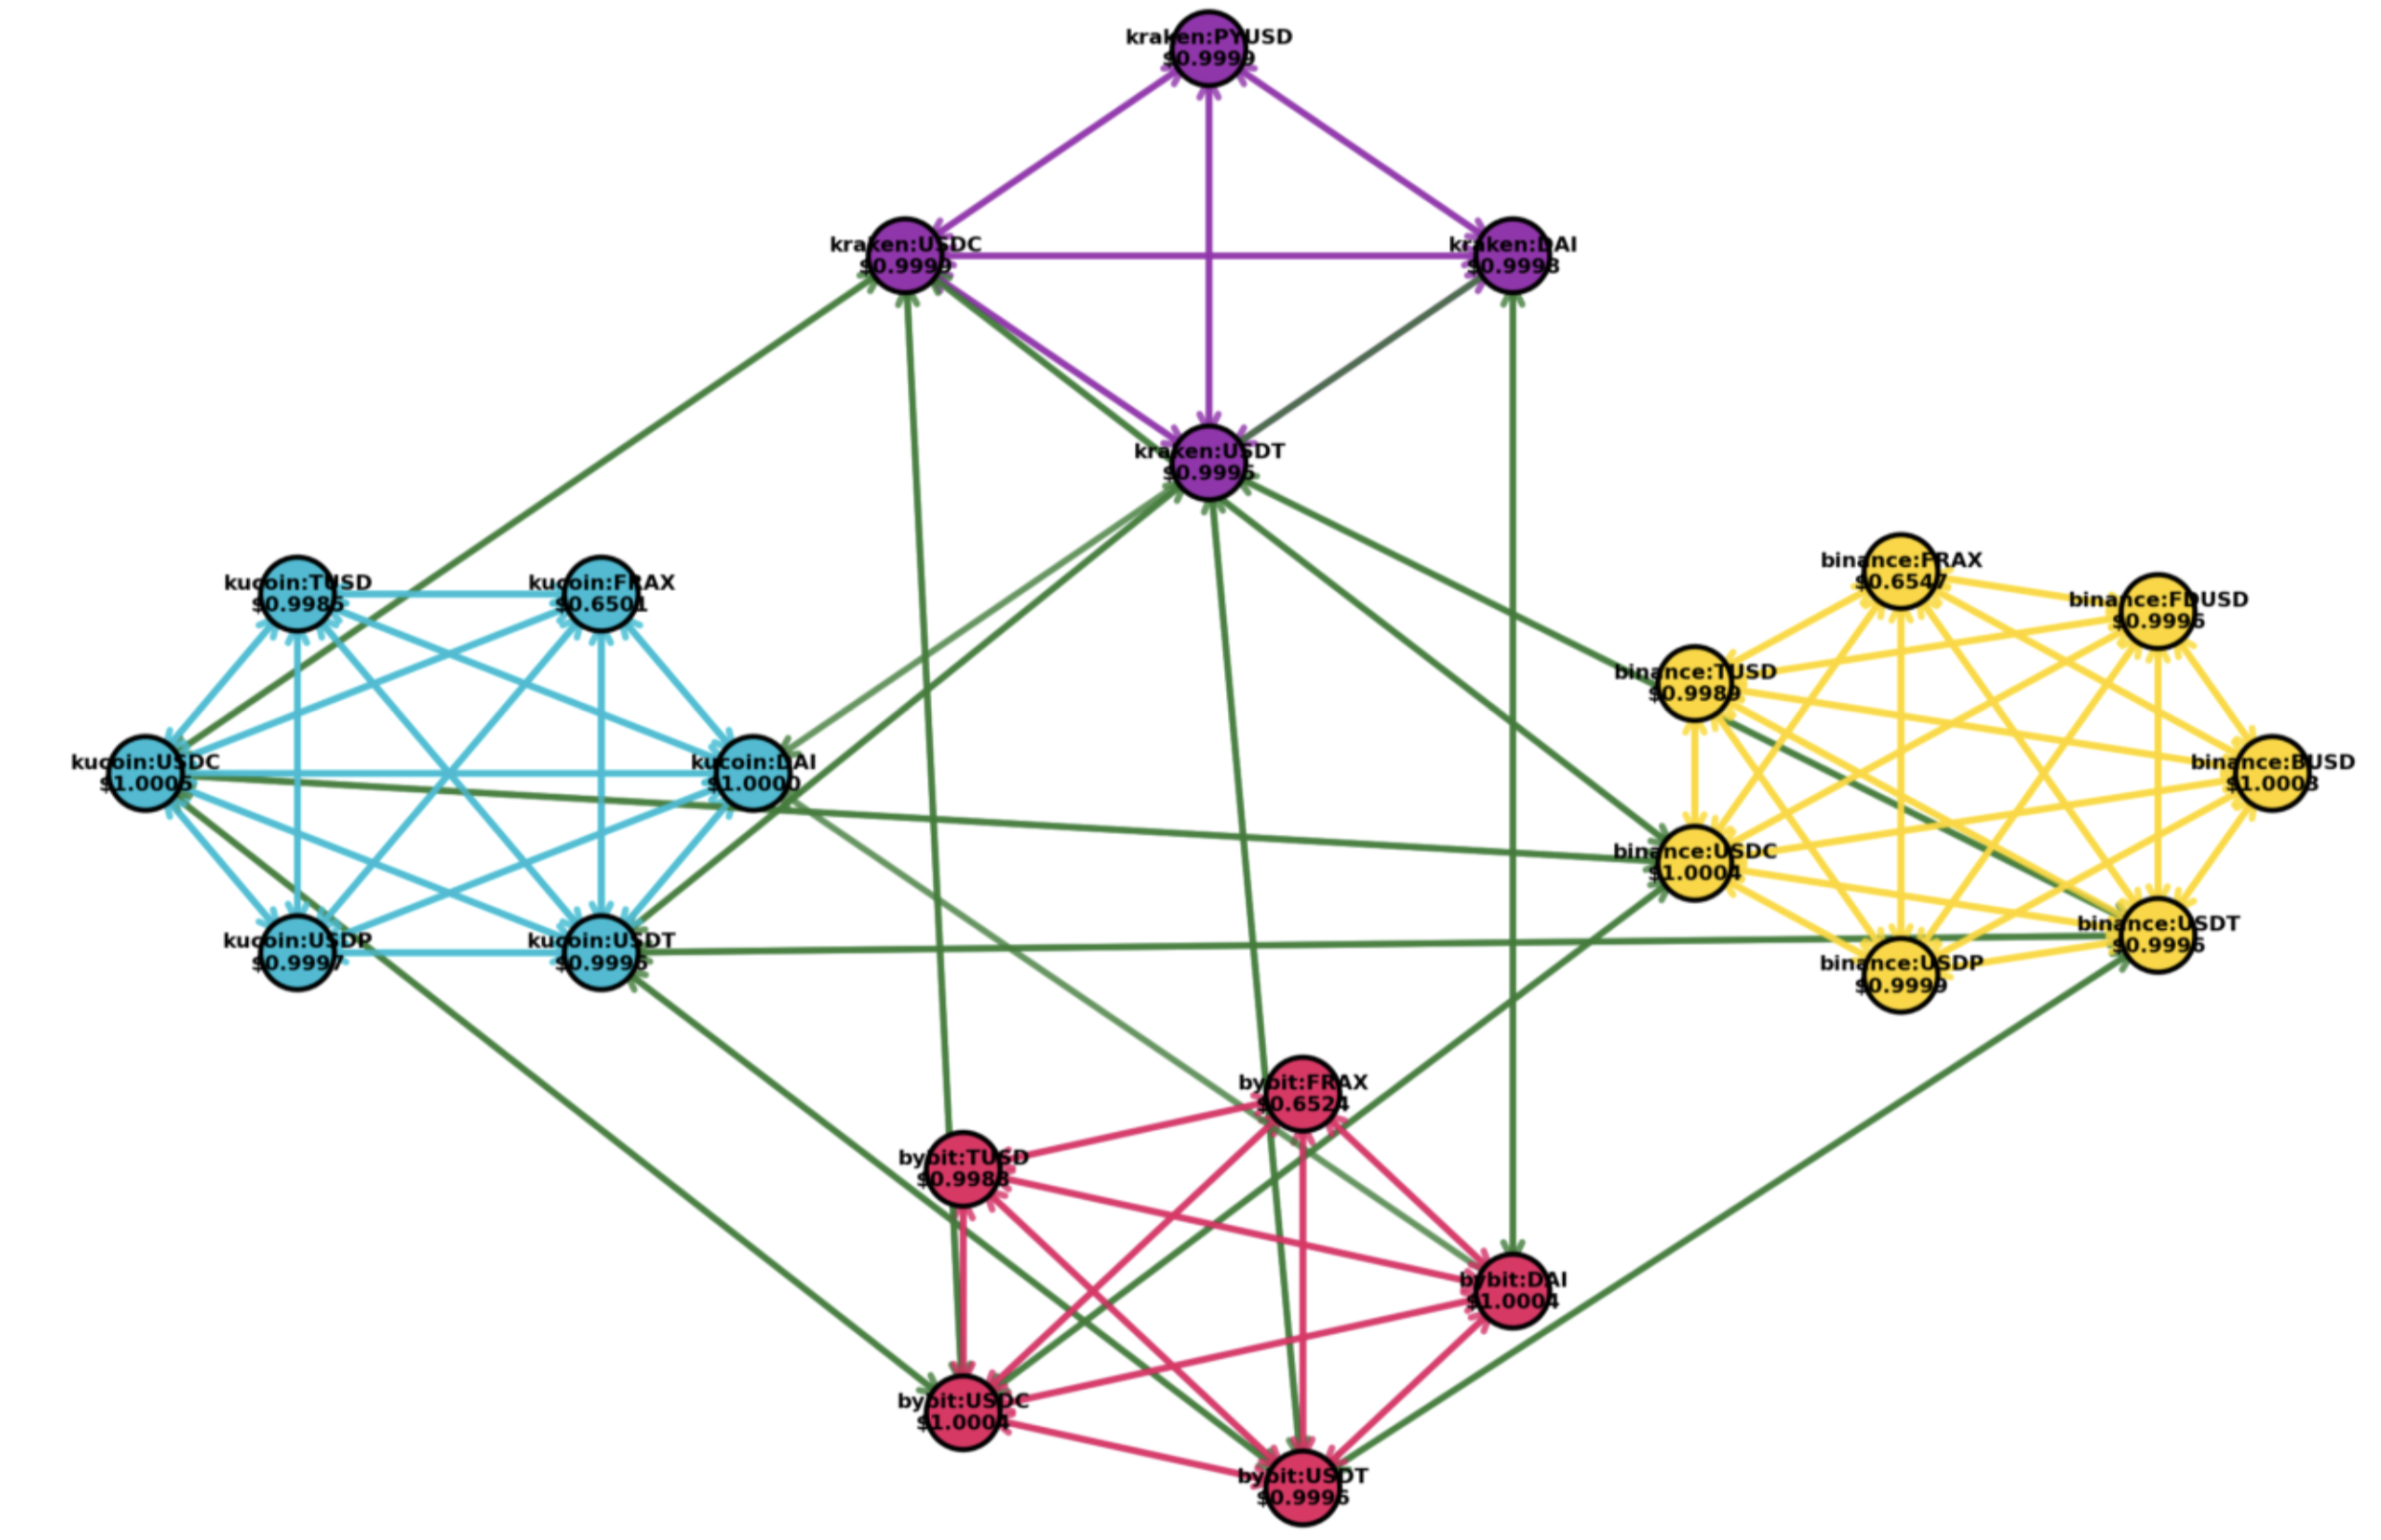
\includegraphics[width=0.85\textwidth]{figures/CoverPageGraphPaper.png}
    \caption{
    Overview of the cross-exchange arbitrage graph used in our experiments.
    Nodes represent (exchange, asset) pairs. Intra-exchange edges denote trading pairs,
    while inter-exchange edges represent asset transfers.
    }
    \label{fig:cover_graph}
\end{figure}

% ---------------- 1. Introduction ----------------
\section{Introduction}
\subsection{Problem Statement and Research Questions}

Cross-exchange stablecoin arbitrage exploits price differences for the same asset across centralized exchanges. Profitable opportunities depend not only on visible price spreads but also on fees, slippage, transfer delays, liquidity constraints, exchange reliability, and short arbitrage windows. We formulate this as a graph-planning problem and develop an automated route planner that computes complete, executable trade-and-transfer paths rather than simple pairwise price gaps. By incorporating trading fees, withdrawal costs, transfer latencies, liquidity depth, and live market data via CCXT~\cite{ccxt2024}, the system generates execution-ready arbitrage paths. Unlike prior detection tools~\cite{oanta2023crypto}, our approach integrates real-world constraints and applies A* search with domain-specific heuristics.

Our methodology addresses four research questions: (1)~Do certain heuristics consistently outperform others on specific trading-instance classes? (2)~How does each heuristic influence A*'s node-expansion behaviour? (3)~How does performance change as structural difficulty increases (liquidity sparsity, high withdrawal fees, fragmented listings)? (4)~When heuristics return suboptimal routes, how close are they to the best-known solution?

\subsection{Why Cross-Exchange Stablecoin Arbitrage Matters}

Stablecoins serve as the primary liquidity bridges in cryptocurrency markets. Because centralized exchanges operate independently, price discrepancies for the same USD-pegged asset frequently arise due to fragmented liquidity, withdrawal delays, blockchain congestion, and operational frictions. Unlike volatile cryptocurrencies, stablecoins operate within a bounded price band anchored to fiat currency, reframing arbitrage from speculative price prediction into a constrained execution-optimization problem where path-dependent execution costs dominate expected return.

During periods of macroeconomic instability, stablecoin flows intensify as capital migrates toward dollar-pegged assets, amplifying cross-exchange imbalances and increasing both spread frequency and execution complexity.

\subsection{Key Challenges}

Cross-exchange arbitrage is constrained by several real-world frictions.
\textbf{Liquidity:} order-book depth determines deployable capital without market impact.
\textbf{Slippage:} large orders incur nonlinear price impact, so theoretical profit often differs from realized profit.
\textbf{Latency:} blockchain confirmations may exceed the arbitrage window.
\textbf{Reliability:} exchanges may experience withdrawal suspensions or API instability.
These constraints interact: faster chains may reduce latency but carry higher reliability risk. Our heuristic-guided A* framework models these trade-offs to prioritize routes that are not only theoretically profitable but realistically executable.



% ---------------- 2. Related Work ----------------
\section{Related Work}
Cryptocurrency arbitrage has been studied from multiple perspectives. Most prior work focuses on identifying arbitrage opportunities, while comparatively less attention has been devoted to modeling execution feasibility under real-world constraints.

\paragraph{Graph-theoretic arbitrage detection.}
The dominant formulation models financial markets as directed weighted graphs where the log transform $w(e)=-\log(r(e))$ converts multiplicative rates into additive costs, so arbitrage opportunities correspond to negative-weight cycles detectable by Bellman--Ford~\cite{bellman1958routing,cormen2009introduction}. Oant\u{a} and Coroiu~\cite{oanta2023crypto} adopt this paradigm in \emph{Crypto Advisor}, aggregating real-time exchange data to detect arbitrage cycles. Similar graph-based formulations appear in DeFi systems~\cite{defiposer2021}, improved negative-cycle algorithms~\cite{mmbf2024,rich2025}, and high-frequency frameworks~\cite{fang2022cryptocurrency}. Across these works, the core objective is opportunity detection rather than execution-aware feasibility.

\paragraph{Execution feasibility and market frictions.}
Single-exchange optimal execution has been studied using reinforcement learning and stochastic control~\cite{kearns2006reinforcement,optimalexecution2024}. Cross-exchange arbitrage introduces additional constraints: blockchain transfer latency, withdrawal fees, liquidity fragmentation, and exchange reliability. Stablecoin markets are particularly sensitive to these frictions due to narrow spreads. Obadia et~al.~\cite{obadia2021flashbots} show that on-chain arbitrage profits are highly sensitive to transaction ordering and confirmation latency; in the CEX-to-CEX setting, withdrawal processing and blockchain finality delays add further uncertainty.

\paragraph{Risk-aware pathfinding and slippage.}
Nikolova and Karger~\cite{nikolova2008stochastic} study risk-averse pathfinding under stochastic edge weights, and Lim et~al.~\cite{lim2022cvar} propose CVaR pathfinding to minimize worst-case tail cost. Our $h_4$ heuristic addresses a similar concern by penalizing unreliable exchanges and congested chains. For slippage, execution cost increases with order size in both AMMs and CEX order books. Our $h_2$ heuristic estimates slippage via live VWAP computation, avoiding parametric assumptions; more advanced models such as Almgren and Chriss~\cite{almgren2001optimal} are left for future work.

\paragraph{Positioning.}
In contrast to prior work, our approach integrates feasibility modeling directly into A* search with domain-specific guidance heuristics, bridging opportunity detection and executable route construction for the low-margin stablecoin context.



% ---------------- 3. Problem Formulation ----------------
\section{Problem Formulation}
\subsection{Graph Representation}

We formulate the stablecoin cross-exchange arbitrage problem as a directed weighted graph
$G=(V,E)$. Each node $v\in V$ represents a unique stablecoin--exchange pair, written as
$v=(exchange,coin)$. Each directed edge $e\in E$ corresponds either to a trade executed on an
exchange or a transfer of funds between exchanges. 

Every edge has an associated effective exchange rate that incorporates all relevant costs---including trading fees, withdrawal fees, spreads, and slippage. We assign each edge a weight using the negative logarithm of this effective rate:
\[
w(e) = -\log\!\big(\textit{effective\_rate}(e)\big).
\] % this can be inline

This transformation converts multiplicative returns into additive costs, enabling the use of shortest-path algorithms to evaluate profitability.

\subsection{Path Profitability}

Given a path $P=(v_0,v_1,\dots,v_k)$ with initial capital $C_0$, the final capital after executing all trades and transfers along the path is
\[
C_k = C_0 \cdot \prod_{e\in P} r(e)
\]
where $r(e)$ denotes the effective rate on edge $e$. A path is profitable when the net gain exceeds a user-specified minimum profit threshold:
\[
C_k - C_0 \ge \textit{min\_profit}.
\] % this can be inline 

Expressing this condition in additive log space gives an equivalent constraint:
\[
\sum_{e\in P} -\log\!\big(r(e)\big)
\;\le\;
-\log\!\left(1+\frac{\textit{min\_profit}}{C_0}\right).
\]

Thus, the arbitrage search problem becomes the task of identifying a path that begins at a given start node $v_0$ and ends at some end node $v_k$, and yields a multiplicative return greater than one. More formally, we seek:
\[
\textit{Find } P: v_0 \to v_k \;\; \textit{s.t.}\;\; \prod_{e\in P} r(e) > 1
\]
This constitutes a minimum-cost path search under realistic execution constraints.

\paragraph{Goal Condition.}
We define the \emph{goal set} $\mathcal{G}$ as the set of all nodes reachable from the start node $v_0$ at which the accumulated capital exceeds the initial capital:
\[
\mathcal{G} = \bigl\{\, v_k \in V \;\big|\; C_k = C_0 \cdot \textstyle\prod_{e \in P} r(e) > C_0 \,\bigr\}.
\]
Critically, we do \emph{not} require $v_k = v_0$. This is an \textbf{open-path} formulation: the trader may end on any exchange--coin pair where the marked-to-market USD value of the position exceeds the initial capital.

This design is economically justified because all assets in our graph are stablecoins pegged to USD. The terminal position $v_k = (\text{exchange}_k, \text{coin}_k)$ holds a stablecoin whose value is within a narrow band of \$1.00 by construction (we enforce a price tolerance of $\pm 2\%$ when building the graph). Therefore, ``profit'' at any terminal node is realized value: the trader holds $C_k$ units of a USD-pegged asset, and $C_k - C_0$ is the net gain. No additional conversion step is needed to ``close'' the position into USD.

Standard arbitrage literature typically requires closed cycles ($v_k = v_0$), but this restriction is unnecessarily limiting in the stablecoin domain. A profitable open path—for example, starting with USDT on Binance and ending with USDC on Kraken—yields the same economic outcome as a closed cycle, because both endpoints hold fungible USD-denominated value. Our formulation therefore maximizes the opportunity set without sacrificing profit interpretation.

\subsection{A* Search Formulation}

To solve the arbitrage problem efficiently, we apply the A* search algorithm. For each node $n$, we maintain a cost-to-reach value $g(n)$, computed as the sum of the additive edge costs encountered so far:
\[
g(n) = \sum_{e\in path} -\log\!\big(r(e)\big).
\]

We define a heuristic function $h(n)$ that estimates the remaining cost or execution risk required to complete a profitable cycle. The A* evaluation function is given by
\[
f(n) = g(n) + h(n),
\]
where $g(n)$ denotes the accumulated path cost in log space and $h(n)$ estimates the remaining cost to complete a feasible arbitrage path. The algorithm terminates when a path yields final capital exceeding the initial capital, that is, when $C_n > C_0$. This formulation allows A* to balance realized execution costs with heuristic estimates of remaining feasibility and risk.

\paragraph{Heuristic Design Philosophy.}
In standard A*, optimality is guaranteed when the heuristic $h(n)$ is \emph{admissible}, i.e., $h(n) \leq h^*(n)$ for all nodes $n$, where $h^*(n)$ is the true remaining cost to the nearest goal. In our domain, however, $h^*(n)$ is not well-defined for two reasons: (i) the goal set $\mathcal{G}$ depends on the \emph{accumulated capital} along the path (not just the current node), and (ii) market conditions change over time, so edge costs are not truly static.

We therefore design our heuristics $h_1$--$h_4$ as \textbf{guidance penalties} rather than admissible lower bounds. Each heuristic $h_i(n) \geq 0$ penalizes execution-risk features (illiquidity, slippage, chain congestion, exchange unreliability) at a given node. These penalties steer A* toward paths that are more likely to remain profitable under real-world conditions, even though they do not satisfy the formal admissibility condition $h(n) \leq h^*(n)$.

For the chain congestion and exchange reliability heuristic ($h_4$), we employ \textbf{Weighted A*} with the evaluation function:
\[
f(n) = g(n) + w(n) \cdot h(n), \quad w(n) \in [w_{\min}, w_{\max}],
\]
where $w(n)$ is a node-specific weight computed from the chain kickback risk score $\rho(n) \in [0,1]$ as:
\[
w(n) = w_{\min} + (w_{\max} - w_{\min}) \cdot \rho(n).
\]
In our experiments, we set $w_{\min} = 1.0$ and $w_{\max} = 3.0$. Fast-transfer chains (high $\rho$) receive higher weight, penalizing paths that traverse chains where arbitrage opportunities are likely to vanish before execution completes. When $w(n)=1$ for all nodes, Weighted A* reduces to standard A*.

\paragraph{Completeness.}
The algorithm is not complete: market data does not guarantee the existence of a profitable path from every starting node $v \in V$. The search terminates either when a profitable path is found, when the search frontier is exhausted, or when depth/time limits are reached.


\subsection{Demonstrative Example}

Consider a simplified arbitrage graph with three nodes: $\text{binance:USDT}$, $\text{kucoin:USDT}$, and $\text{kucoin:TUSD}$. Suppose we have the following edges with effective rates:

\begin{itemize}
\item $\text{binance:USDT} \to \text{kucoin:USDT}$: rate $r_1 = 0.9995$ (includes transfer fee)
\item $\text{kucoin:USDT} \to \text{kucoin:TUSD}$: rate $r_2 = 1.0042$ (profitable trade)
\item $\text{kucoin:TUSD} \to \text{binance:USDT}$: rate $r_3 = 0.9995$ (transfer back)
\end{itemize}

\begin{figure}[t]
    \centering
    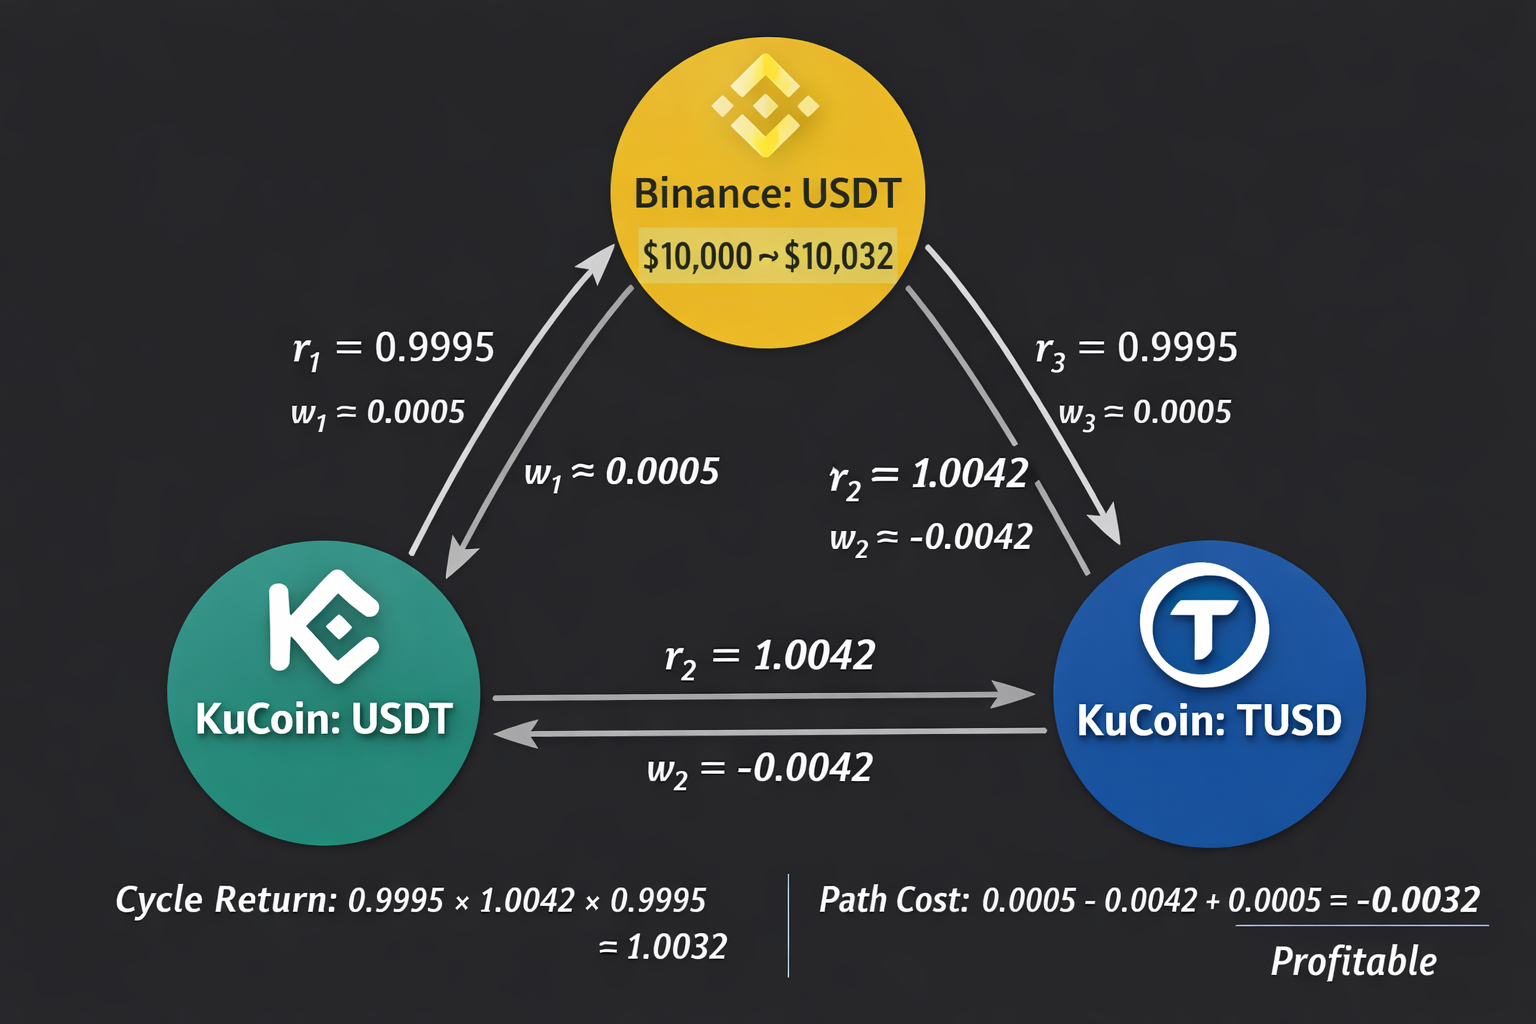
\includegraphics[width=0.9\linewidth]{figures/arbitrage_path.png}
    \caption{
    Simplified three-node arbitrage cycle across Binance and KuCoin.
    Edge labels denote effective multiplicative rates $r_i$ and corresponding
    log-space weights $w_i = -\log r_i$. The total log-cost of the cycle is
    negative, indicating a theoretical profitable arbitrage opportunity. It is important to note, our research is not constrained to profitable cycles, and is allows for any profitable path to represent a goal state.
    }
    \label{fig:arbitrage_example}
\end{figure}


The cycle $\text{binance:USDT} \to \text{kucoin:USDT} \to \text{kucoin:TUSD} \to \text{binance:USDT}$ has a multiplicative return of:
\[
\prod_{e\in P} r(e) = 0.9995 \times 1.0042 \times 0.9995 \approx 1.0032
\]

Starting with \$10,000, the final capital would be approximately \$10,032, yielding a profit of \$32. The edge weights in log space are:
\begin{align}
w_1 &= -\log(0.9995) \approx 0.0005 \\
w_2 &= -\log(1.0042) \approx -0.0042 \\
w_3 &= -\log(0.9995) \approx 0.0005
\end{align}

The total path cost is $0.0005 - 0.0042 + 0.0005 = -0.0032$, which is negative, indicating a profitable cycle (negative cost in log space corresponds to positive return).

\begin{figure}[ht]
    \centering
    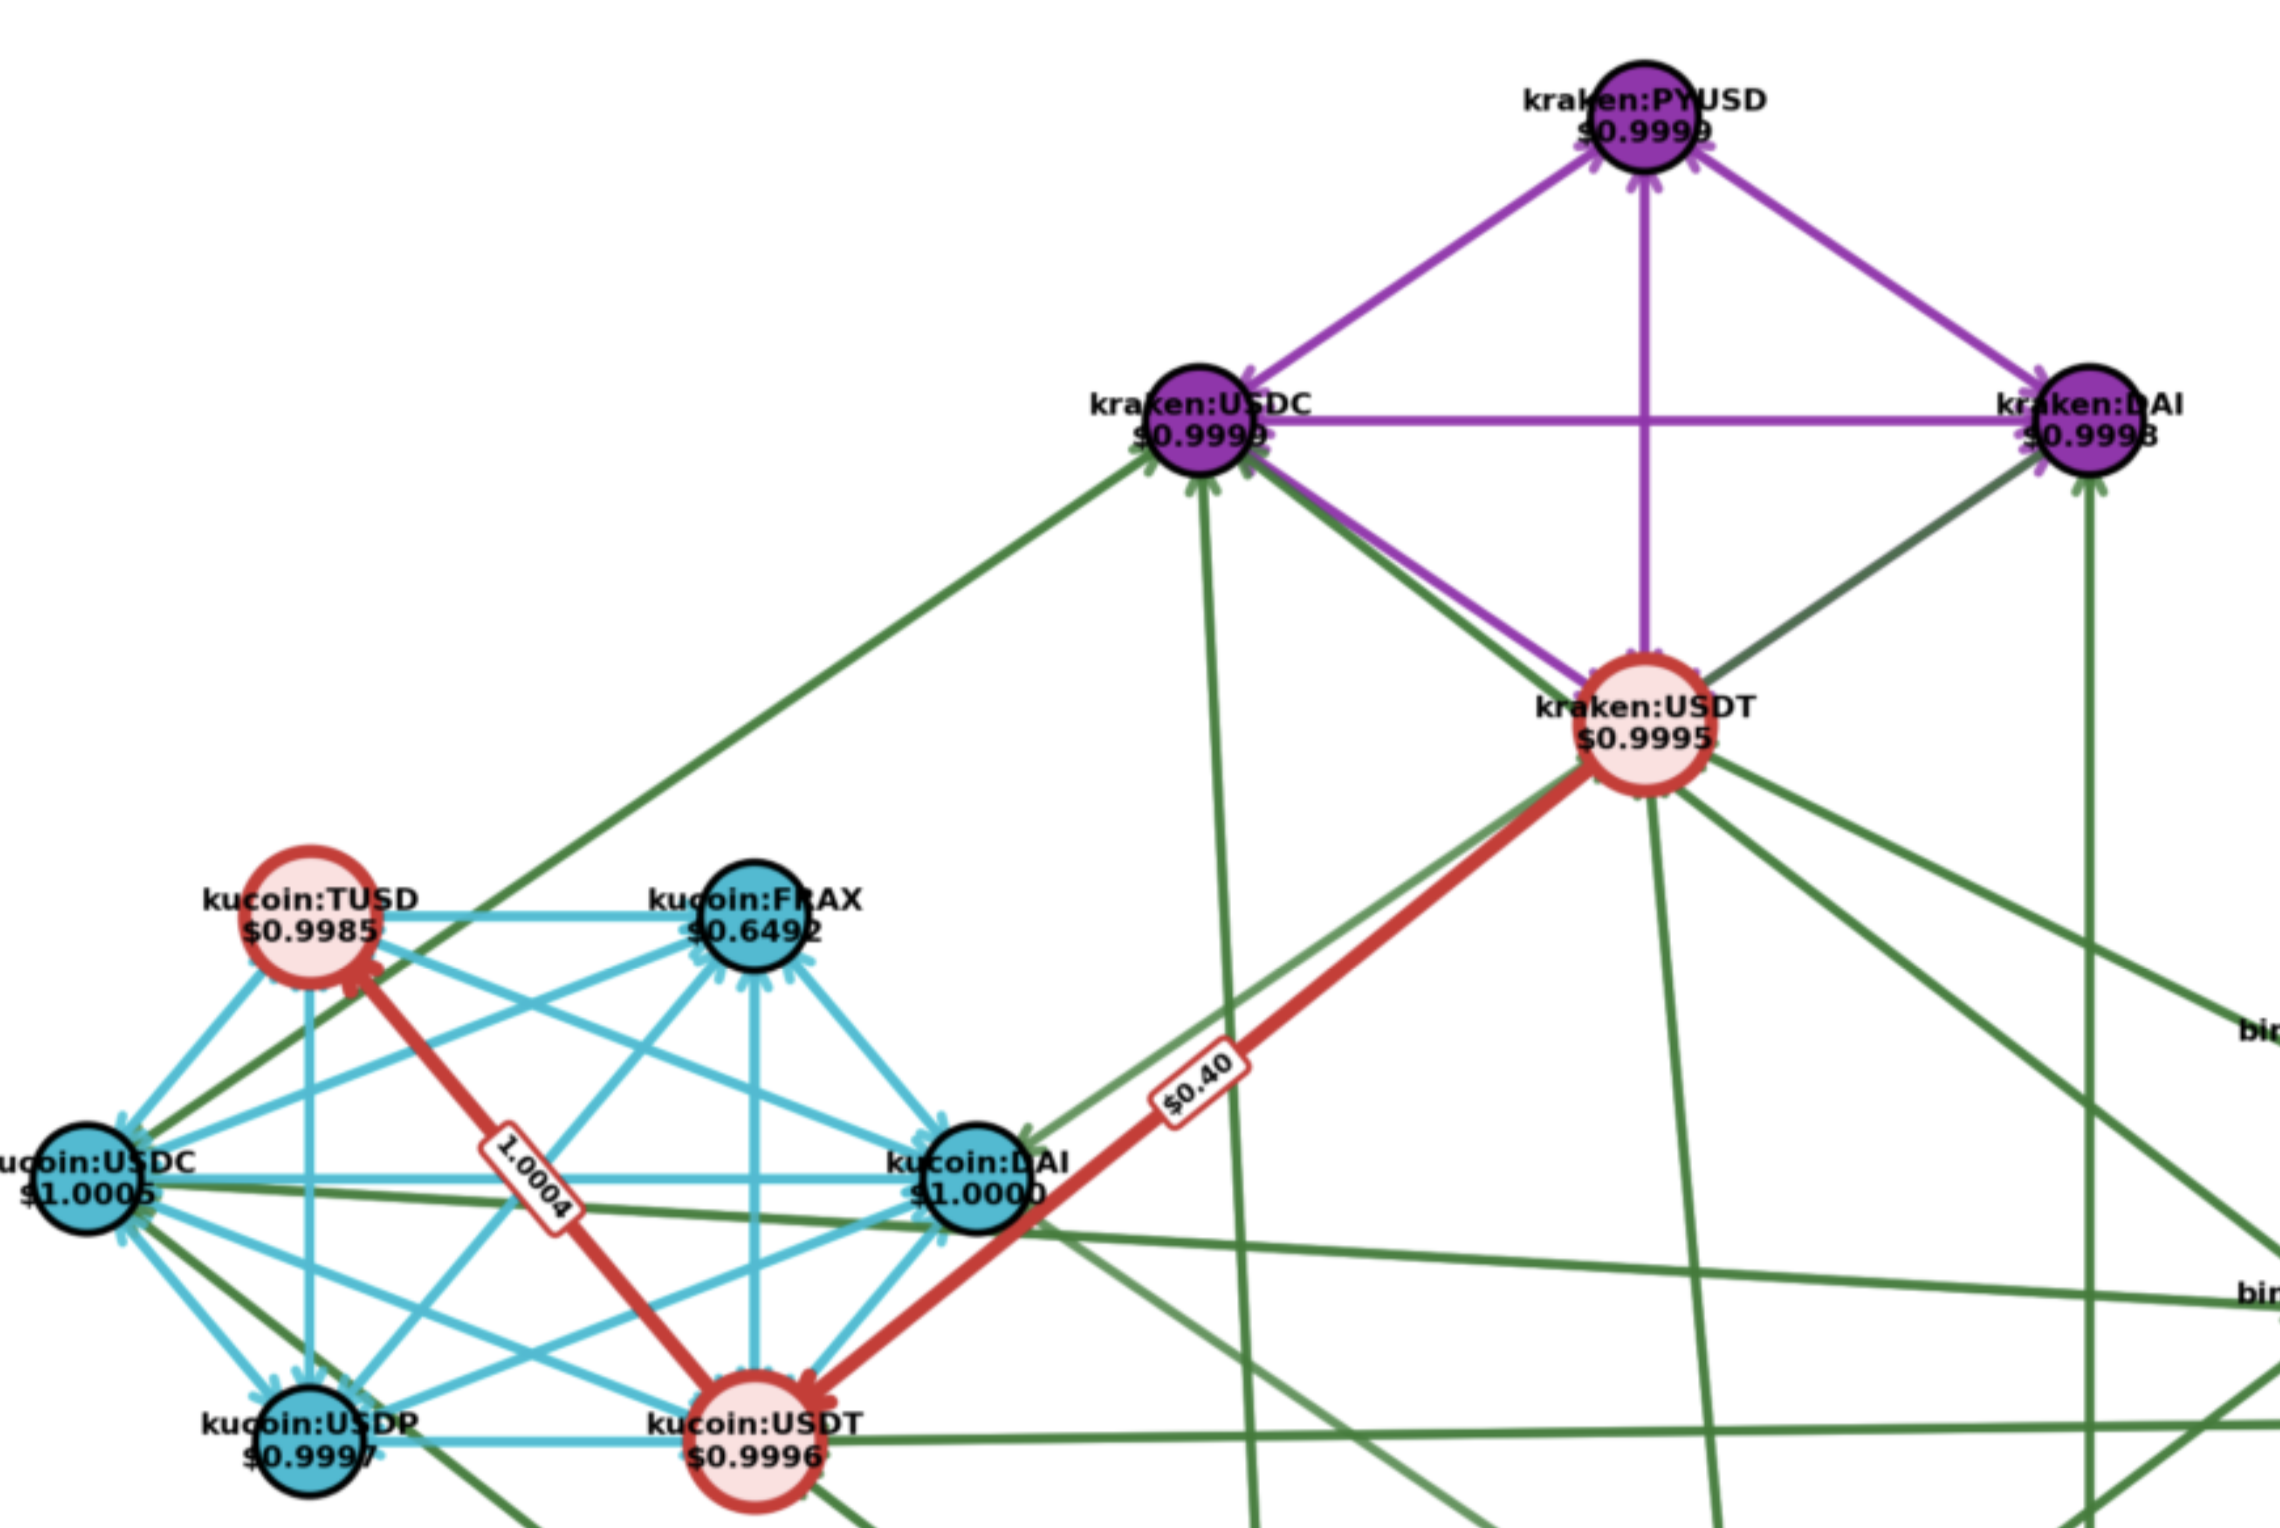
\includegraphics[width=0.85\textwidth]{figures/SuccesfulPathProfit}
    \caption{
    Visualization of a successful arbitrage path identified by our search algorithm.
    The path shows a sequence of trades and transfers across multiple exchanges,
    starting from the initial node and following the highlighted edges to complete
    a profitable cycle. Each node represents an (exchange, asset) pair, with node
    colors indicating the exchange. The bold red edges trace the optimal route,
    with edge labels showing the exchange rates for trades and transfer fees for
    cross-exchange movements. This simplified view isolates the profitable path
    from the full graph structure, demonstrating how the algorithm navigates
    through the arbitrage opportunity space.
    }
    \label{fig:successful_path}
\end{figure}




% ---------------- 4. Novel Heuristics ----------------
\section{Novel Heuristics for Arbitrage Search}
We design three domain-specific guidance heuristics ($h_1$, $h_2$, $h_4$) and one search-control strategy ($h_3$) to guide A* toward reliable, low-risk, and realistically executable arbitrage routes. Each heuristic captures a different dimension of execution feasibility. Rather than detecting theoretical profit first and evaluating risk afterward, our approach embeds execution awareness directly into the search process.

Each node-level heuristic modifies the evaluation function
\[
f(n) = g(n) + h(n),
\]
where $g(n)$ is the accumulated cost in log space and $h(n) \geq 0$ is an additive guidance penalty encoding domain knowledge about future execution feasibility. As discussed in Section~3, these heuristics are \emph{guidance penalties}: they do not modify $g(n)$ and do not claim admissibility.

\subsection{$h_1$ -- Liquidity Heuristic}

The liquidity heuristic models the risk that low-volume markets cannot support the required trade size without excessive execution impact.

Let
\begin{align}
\textit{vol\_per\_sec}
&=
\frac{\textit{24h\_quote\_volume}}{24 \times 3600}
\\
\textit{liquidity\_ratio}
&=
\frac{\textit{vol\_per\_sec} \cdot T_{\textit{remain}}}
{\textit{order\_size\_usd}}.
\end{align}

This ratio estimates whether expected market flow during the remaining arbitrage window can support the intended order size.

We normalize this quantity into a bounded score:

\[
\textit{score}_{liq} =
\textit{clamp}\!\left(
\frac{\log_{10}(\textit{liquidity\_ratio}) + 1}{2},
0,
1
\right).
\]

The heuristic cost becomes:

\[
h_1(n) = \lambda_{liq} \big(1 - \textit{score}_{liq}(n)\big).
\]

\textbf{Characteristics:}
\begin{itemize}
    \item Time-aware liquidity modeling
    \item Accounts for order size relative to trading activity
    \item Favors deep, actively traded markets
\end{itemize}

This heuristic is well suited for conservative strategies prioritizing reliable execution over aggressive profit maximization.

\subsection{$h_2$ -- Slippage Heuristic}

The slippage heuristic directly models expected execution price impact using real-time order-book depth.

Let $P_{mid}$ denote the mid-price and $\textit{VWAP}(Q)$ the volume-weighted average price required to fill order size $Q$. Slippage in basis points is defined as:

\[
\textit{slippage}_{bps} =
\frac{\textit{VWAP}(Q) - P_{mid}}{P_{mid}} \times 10^{4}.
\]

The heuristic is defined as:

\[
h_2(n) =
\lambda_{slip} \cdot 
\max \left\{ 0, \textit{slippage}_{bps} - \theta \right\},
\]

where $\theta$ is a configurable slippage tolerance (default: 10 bps = 0.10\%).

\paragraph{Relationship to edge costs (no double-counting).}
Edge effective rates $r(e)$ encode \emph{static} costs: the posted taker fee (e.g., 0.10\% on Binance) and withdrawal/gas fees. These fees are deterministic and independent of order size. By contrast, $h_2$ estimates \emph{dynamic} order-book slippage: the price impact of walking the live order book with a specific order size $Q$. Because edges use fixed taker-fee rates rather than order-book-derived VWAP, $h_2$ is additive guidance that captures information not present in $g(n)$, and there is no double-counting.

\textbf{Characteristics:}
\begin{itemize}
    \item Uses real-time order book data
    \item Side-aware (buy vs. sell impact)
    \item Directly penalizes large price impact
    \item Purely additive guidance: does \emph{not} modify $g(n)$
\end{itemize}

This heuristic performs particularly well when order-book depth is the dominant constraint.

\subsection{Multi-Start Search Strategy ($h_3$)}
\label{sec:h3_multistart}

Unlike $h_1$, $h_2$, and $h_4$, which are node-level heuristic functions that return a scalar penalty for each node, $h_3$ is a \textbf{search-control strategy} that operates at the meta-level. It runs multiple independent A* searches concurrently from randomly selected starting nodes, each using a base heuristic (typically $h_1$), and returns the best solution found across all parallel instances.

This strategy is \emph{not} a heuristic in the formal A* sense: it does not define a per-node cost estimate $h_3(n)$, and it does not affect the $f(n) = g(n) + h(n)$ evaluation within any single search. Instead, it addresses a fundamentally different problem: when the profitable region of the graph is unknown a priori, multi-start search diversifies exploration across the state space.

Formally, let $\{v_1, v_2, \dots, v_k\}$ be $k$ randomly sampled starting nodes. For each $v_i$, we run an independent A* search with some base heuristic $h_b \in \{h_1, h_2, h_4\}$:
\[
\text{result}_i = A^*(v_i, h_b), \quad i = 1, \dots, k.
\]
The final output is $\arg\max_{i} \text{profit}(\text{result}_i)$ among successful searches.

\textbf{Characteristics:}
\begin{itemize}
    \item Diversifies search across starting exchanges
    \item Mitigates dependence on a fixed starting point
    \item Embarrassingly parallel (scales with available threads)
    \item Higher total computational cost (linear in $k$)
\end{itemize}

This approach is particularly useful when profitable starting points are not known in advance.

\subsection{$h_4$ -- Chain Congestion and Exchange Reliability Heuristic}

The $h_4$ heuristic incorporates transfer latency and operational reliability into the search.

Let $t_{min}$ denote the shortest outgoing transfer time from the current node, and $T_{remain}$ the remaining arbitrage window. The chain reliability score is:

\[
\textit{score}_{chain} =
1 - \frac{t_{min}}{T_{remain}}.
\]

The corresponding chain penalty is:

\[
h_{chain}(n) =
\lambda_{chain} \big(1 - \textit{score}_{chain}(n)\big).
\]

If each exchange is assigned a reliability score $s(n) \in [0,1]$, we define:

\[
h_{exchange}(n) =
\lambda_{exchange} \big(1 - s(n)\big).
\]

The combined heuristic is:

\[
h_4(n) = h_{chain}(n) + h_{exchange}(n).
\]

\paragraph{Chain transfer times.}
Transfer-time estimates $t_{\min}$ are drawn from documented blockchain finality times plus typical exchange processing delays. For example: Solana $\approx$~1\,s, BNB Chain $\approx$~4\,s, Polygon $\approx$~5\,s, Tron $\approx$~30\,s, Arbitrum/Base $\approx$~120\,s, Ethereum $\approx$~600\,s.

\paragraph{Weighted A* with $h_4$.}
As described in Section~3, $h_4$ is used with Weighted A*. The node-specific weight $w(n)$ amplifies the heuristic penalty for nodes on fast-transfer chains where arbitrage opportunities are fleeting.

\textbf{Characteristics:}
\begin{itemize}
    \item Models blockchain congestion and finality risk
    \item Incorporates exchange operational reliability
    \item Uses Weighted A* ($w \in [1.0, 3.0]$) for risk-adaptive search
    \item Prioritizes fast and stable execution paths
\end{itemize}

% ---------------- 5. Experiments ----------------
\section{Experiments and Evaluation}
Our experimental framework constructs a real-time, execution-aware graph representation of stablecoin arbitrage opportunities (see Figure~\ref{fig:cover_graph}).

\subsection{Data Sources and Graph Construction}

We gather live market data from twelve major exchanges (Binance, Kraken, KuCoin, Bybit, OKX, Gate.io, Bitget, MEXC, HTX, Coinbase, Crypto.com, Phemex) via CCXT~\cite{ccxt2024}. Prices are normalized to USD using conservative bid/ask estimates, and a $\pm 2\%$ price tolerance filter excludes depegged assets. The fee model captures taker fees, exchange-specific withdrawal fees per blockchain, and estimated gas fees. Transfer time is modelled as blockchain confirmation time plus 45\,s user execution overhead. All hyperparameters are listed in Appendix~\ref{sec:hyperparams}.

\begin{table*}[t]
\centering
\small
\setlength{\tabcolsep}{6pt}
\caption{Baseline algorithm performance on cached graph (41~nodes, 864~edges, 30~start nodes). 
All profits are net after trading, withdrawal, and gas fees.}
\label{tab:baseline-performance}
\begin{tabular}{lccccccc}
\toprule
\textbf{Baseline} 
& \textbf{Cash} 
& \textbf{Success} 
& \textbf{Avg Profit (\$)} 
& \textbf{Avg Profit (\%)} 
& \textbf{Avg Expand}
& \textbf{Avg Time (s)} 
& \textbf{Max Path Len} \\
\midrule

Dijkstra ($h{=}0$)
& \$1k      & 56.7\% &   1.00 & 0.100\%  & 359 & 0.010 & 3 \\
& \$10k     & 56.7\% &  10.01 & 0.100\%  & 359 & 0.010 & 3 \\
& \$100k    & 56.7\% & 100.07 & 0.100\%  & 359 & 0.010 & 3 \\
\midrule

3-hop enum.
& \$1k      & 30.0\% &   0.54 & 0.054\%  & 346 & $<$0.001 & 3 \\
& \$10k     & 30.0\% &   5.40 & 0.054\%  & 346 & $<$0.001 & 3 \\
& \$100k    & 30.0\% &  54.04 & 0.054\%  & 346 & $<$0.001 & 3 \\
\midrule

\texttt{simple\_1hop}
& All       & 0/30  & -- & -- & -- & $<$0.001 & 1 \\
\midrule

\texttt{simple\_2hop}
& All       & 0/30  & -- & -- & -- & $<$0.001 & 2 \\
\midrule

Bellman--Ford
& All       & 0/30  & -- & -- & -- & $<$0.001 & -- \\

\bottomrule
\end{tabular}
\end{table*}

% ---------------- 5.2 Baseline Algorithms (Non-A*) ----------------
% ---------------- 5.2 Ablation Studies ----------------
\subsection{Ablation Studies on A*}

To isolate the contribution of heuristic guidance, we evaluate our approach against three ablation baselines:

\begin{enumerate}
    \item \textbf{Cycle ablation:} We force classical cycle detection using Bellman--Ford, identifying negative cycles rather than optimizing for executable profitable paths.
    
    \item \textbf{Depth ablation:} We restrict search depth to shallow expansions. 
    The \texttt{simple\_1hop} variant evaluates only single outgoing actions, while 
    \texttt{simple\_2hop} evaluates minimal two-edge loops (the shortest possible cycle).
    
    \item \textbf{Heuristic ablation:} We remove heuristic guidance entirely by setting $h(n)=0$, reducing A* to Dijkstra’s algorithm and eliminating blockchain-aware signals such as congestion, liquidity, and order book depth.
\end{enumerate}


\subsubsection{Bellman--Ford Negative Cycle Detection}
\label{sec:bf-baseline}

We include Bellman--Ford negative-cycle detection as a classical arbitrage baseline. Given edge rates $r(e)$, we apply the log transform
\[
w(e) = -\log(r(e)),
\] % this cna be inline
so multiplicative rate products become additive path costs. Arbitrage opportunities correspond to negative-weight cycles. Bellman--Ford detects whether such a cycle exists in the transformed graph.

In our setting, Bellman--Ford is treated as a \emph{detection} method rather than an execution planner: it does not optimize for order-size-dependent slippage, transfer latency windows, or reliability constraints, and therefore frequently fails to produce an executable profitable cycle under real-world frictions.

\subsubsection{Greedy Spread-Based Strategy}
\label{sec:greedy-baseline}

We include shallow greedy baselines intended to emulate rapid spread scanning:

\begin{itemize}
    \item \textbf{1-hop edge scan (\texttt{simple\_1hop}):} tests whether any single outgoing action yields immediate positive gain. This is a minimal local check and typically cannot complete a full arbitrage cycle.
    \item \textbf{2-hop loop scan (\texttt{simple\_2hop}):} tests whether a two-action sequence can return to the original asset (a minimal loop-back).
\end{itemize}

These strategies are extremely fast, but they generally fail under realistic fees and transfer costs because profitable cross-exchange opportunities typically require coordinated trade+transfer actions.

\subsubsection{Dijkstra / Shortest Path Variant}
\label{sec:dijkstra-baseline}

We implement an unguided shortest-path baseline equivalent to A* with a zero heuristic:
\[
h(n) = 0.
\] % this thingy can be inline 
This reduces A* to Dijkstra’s algorithm, expanding nodes in non-decreasing accumulated cost $g(n)$. The baseline uses the same execution-aware edge model as our proposed methods (fees, withdrawals, gas, and transfer-time penalties encoded into $r(e)$), but provides no heuristic guidance.

Dijkstra represents the most accurate static-cost optimum: its paths are exact under the market data at search time, but may deviate under execution when accounting for dynamic frictions such as order-book slippage and quote staleness.


% ---------------- 5.5.1 Cached-Graph Heuristic Comparison ----------------
\subsubsection{Cached-Graph Heuristic Comparison}
\label{sec:deterministic-compare}

We compare all heuristics and baselines on a \emph{cached} graph snapshot (41~nodes, 864~edges) with 30 randomly selected start nodes and three cash levels, isolating search computation from API I/O. Table~\ref{tab:heuristic-performance} reports aggregate performance.

\begin{table*}[t]
\centering
\small
\setlength{\tabcolsep}{5pt}
\caption{Cached-graph heuristic comparison (41~nodes, 864~edges, 30~start nodes per cash level). Success rate, conditional average profit, mean node expansions, and compute time (I/O excluded). Expansion reduction is relative to Dijkstra.}
\label{tab:heuristic-performance}
\begin{tabular}{llcrrrc}
\toprule
\textbf{Heuristic} 
& \textbf{Cash} 
& \textbf{Success} 
& \textbf{Avg Profit (\$)} 
& \textbf{Avg Expand} 
& \textbf{Avg Time (s)} 
& \textbf{Exp.\ $\Delta$ vs Dijkstra} \\
\midrule

Dijkstra ($h{=}0$)
& \$1k      & 56.7\% &   1.00 &  359 & 0.010 & --- \\
& \$10k     & 56.7\% &  10.01 &  359 & 0.010 & --- \\
& \$100k    & 56.7\% & 100.07 &  359 & 0.010 & --- \\
\midrule

$h_1$ (liquidity)
& \$1k      & 56.7\% &   0.67 &  319 & 0.172 & $+$11.2\% \\
& \$10k     & 56.7\% &   6.72 &  568 & 0.016 & $-$58.0\% \\
& \$100k    & 56.7\% &  63.11 &  715 & 0.021 & $-$98.9\% \\
\midrule

$h_2$ (slippage)
& \$1k      & 56.7\% &   0.99 &  256 & 0.221 & $+$28.8\% \\
& \$10k     & 56.7\% &   9.91 &  256 & 0.011 & $+$28.8\% \\
& \$100k    & 56.7\% & 100.07 &  252 & 0.012 & $+$29.9\% \\
\midrule

$h_4$ (Weighted A*)
& \$1k      & 56.7\% &   0.71 &  673 & 0.020 & $-$87.4\% \\
& \$10k     & 56.7\% &   7.06 &  673 & 0.022 & $-$87.4\% \\
& \$100k    & 56.7\% &  70.58 &  673 & 0.022 & $-$87.4\% \\
\midrule

3-hop enum.
& \$1k      & 30.0\% &   0.54 &  346 & 0.000 & $+$3.6\% \\
& \$10k     & 30.0\% &   5.40 &  346 & 0.000 & $+$3.6\% \\
& \$100k    & 30.0\% &  54.04 &  346 & 0.000 & $+$3.6\% \\

\bottomrule
\end{tabular}
\end{table*}

Several key observations emerge from the cached-graph comparison:

\paragraph{$h_2$ is the most effective heuristic for search pruning.}
$h_2$ achieves a consistent \textbf{29\% reduction in node expansions} relative to Dijkstra across all cash levels, while discovering paths with nearly identical profit (within 1\% at \$100k). Order-book depth information effectively prunes low-liquidity branches.

\paragraph{$h_4$ explores more nodes but provides risk-aware guidance at zero I/O cost.}
$h_4$ expands 87\% more nodes than Dijkstra because its penalty terms (chain congestion + exchange reliability) force the search to evaluate risk-adjusted alternatives. However, its compute time (0.020--0.022\,s) is \emph{comparable to Dijkstra} because it uses pre-computed chain transfer times and static exchange reliability scores with no API calls during search. The paths it discovers are longer (5--6~hops vs.\ 3) and route through more reliable exchanges, at the cost of lower profit.

\paragraph{$h_1$ behaviour is cash-size-dependent.}
At small order sizes (\$1k), $h_1$ achieves 11\% fewer expansions than Dijkstra, but at large sizes (\$100k) it expands 99\% more nodes. The liquidity ratio $\text{vol}/\text{order\_size}$ shrinks for larger orders, activating stronger penalties that force broader exploration.

\begin{table*}[t]
\centering
\small
\setlength{\tabcolsep}{5pt}
\renewcommand{\arraystretch}{1.15}
\caption{Representative execution-ready profitable paths from cached-graph experiments (41~nodes, 864~edges, \$1{,}000 order size). Paths illustrate the different trade-offs each method makes: Dijkstra and $h_2$ find short, high-profit paths; $h_4$ routes through more reliable exchanges at the cost of profit.}
\label{tab:heuristic-profitable-paths}
\begin{tabular}{lclp{0.38\linewidth}rcc}
\toprule
\textbf{Method} 
& \textbf{Start} 
& \textbf{Hops}
& \textbf{Path Description} 
& \textbf{Expand}
& \textbf{Net (\$)} 
& \textbf{Time (s)} \\
\midrule

Dijkstra
& \texttt{phemex:USDT}
& 3
& Transfer phemex$\to$kucoin (USDT on SOL); Trade USDT$\to$TUSD (0.10\% taker).
& 410
& 1.14
& 0.020 \\

\midrule

$h_2$
& \texttt{phemex:USDT}
& 3
& Transfer phemex$\to$kucoin (USDT on SOL); Trade USDT$\to$TUSD (0.10\% taker).
& 209
& 1.14
& 4.752 \\

\midrule

$h_1$
& \texttt{phemex:USDT}
& 3
& Transfer phemex$\to$kucoin (USDT on SOL); Trade USDT$\to$TUSD (0.10\% taker).
& 392
& 1.14
& 4.227 \\

\midrule

$h_4$
& \texttt{phemex:USDT}
& 5
& Longer path through higher-reliability exchanges (Binance, KuCoin); avoids low-reliability intermediaries.
& 606
& 0.98
& 0.017 \\

\bottomrule
\end{tabular}
\end{table*}



% ---------------- 5.4 Evaluation Methodology ----------------
\subsection{Evaluation Methodology}
\label{sec:evaluation}

We evaluate our algorithms along five dimensions: deterministic heuristic comparison on cached graph snapshots, graph scaling behaviour, temporal robustness over multi-hour campaigns, quote staleness analysis under execution delay, and hyperparameter sensitivity.

% ---------------- 5.4.1 ----------------
\subsubsection{Test Environment}

Unless otherwise stated, all experiments use the following configuration:

\begin{itemize}
    \item \textbf{Exchanges:} 12 CEXs (Binance, Kraken, KuCoin, Bybit, OKX, Gate.io, Bitget, MEXC, HTX, Coinbase, Crypto.com, Phemex).
    \item \textbf{Graph:} 41 nodes (exchange$\times$stablecoin pairs), 864 directed edges (trades + transfers).
    \item \textbf{Start nodes:} 30 randomly selected nodes for cached-graph experiments; 5 preferred major-exchange nodes for overnight and scaling experiments (see Table~\ref{tab:hyperparams} for all search parameters).
    \item \textbf{Cash levels:} \$1{,}000, \$10{,}000, \$100{,}000.
    \item \textbf{Heuristics tested:} $h_1$ (liquidity), $h_2$ (slippage), $h_4$ (chain/exchange risk via Weighted~A*), Dijkstra ($h{=}0$), and 3-hop enumeration baseline.
\end{itemize}

\paragraph{Cached vs.\ live experiments.}
A key methodological distinction is between \emph{cached} and \emph{live} experiments. In cached experiments, the graph is built once from a live price snapshot and then all heuristics search on the \emph{same frozen graph}, isolating algorithmic differences from API I/O latency. In live experiments (overnight, staleness), each snapshot triggers fresh API calls, so wall-clock times include data-acquisition overhead. We report both, as the latency profile of each heuristic is itself a key finding (Section~\ref{sec:overnight}).

% ---------------- 5.4.2 ---------------
\subsubsection{Performance Metrics}

We report six standardized metrics across all experiments:

\begin{enumerate}
    \item \textbf{Success Rate}: $\frac{\text{\# profitable runs}}{\text{\# total runs}}$.
    \item \textbf{Conditional Avg.\ Profit}: $\mathbb{E}[\text{Profit} \mid \text{Success}]$, net of trading, withdrawal, and gas fees.
    \item \textbf{Node Expansions}: number of nodes popped from the open list (measures search effort independent of I/O).
    \item \textbf{Wall-Clock Time}: end-to-end search time including any heuristic API calls (mean, median, and P99 reported separately).
    \item \textbf{Path Length}: number of nodes in the discovered path.
    \item \textbf{Path Type}: whether the path is intra-exchange (2~nodes, single trade) or cross-exchange ($\geq$3~nodes, involving transfers). We report both categories separately to distinguish trivial single-exchange mispricings from genuine cross-exchange arbitrage.
\end{enumerate}

Profit statistics are conditioned on successful runs; failed runs are reflected only in the success rate. This separation avoids diluting economic performance metrics with zero-profit failures.

\subsection{Results}

\subsubsection{Deterministic Heuristic Comparison}

We evaluate all heuristics on a cached graph snapshot (41~nodes, 864~edges) from 30 randomly selected start nodes at three cash levels (\$1k, \$10k, \$100k), totalling 90~runs per method. By freezing the graph, we isolate algorithmic differences from API latency. Full results are reported in Table~\ref{tab:heuristic-performance}; we summarise the key findings here.

All A*-based methods achieve identical success rates (56.7\%), confirming that heuristic choice does not affect \emph{whether} a profitable path exists, only \emph{which} path is found and how efficiently. The 3-hop enumeration baseline succeeds for only 30\% of start nodes because it cannot discover 2-hop intra-exchange opportunities or 4+~hop cross-exchange paths.

$h_2$ (slippage) achieves the best search efficiency, reducing node expansions by \textbf{29\%} relative to Dijkstra across all cash levels while matching Dijkstra's profit within 1\% at large order sizes. This demonstrates that order-book depth information provides effective search guidance.

$h_4$ (Weighted~A*) expands 87\% more nodes than Dijkstra due to its chain-congestion and exchange-reliability penalties, but its wall-clock compute time (0.020--0.022\,s) is comparable to Dijkstra's (0.010\,s) because it makes \emph{zero API calls} during search. The additional expansions produce longer paths (5--6~hops) that route through higher-reliability exchanges, trading profit for execution safety.

$h_1$ (liquidity) exhibits cash-size-dependent behaviour: at \$1k it reduces expansions by 11\% (the liquidity ratio is favourable), but at \$100k it expands 99\% more nodes (large orders trigger stronger liquidity penalties, forcing broader exploration).

Start node sensitivity persists across all methods: approximately 43\% of randomly chosen start nodes yield no profitable path regardless of heuristic, reflecting structural properties of the fee landscape rather than algorithmic limitations.

\subsubsection{Comparison Against Baselines}

We compare our heuristic-guided A* methods against five baseline algorithms: Dijkstra's algorithm (A* with $h(n) = 0$), brute-force 3-hop enumeration, Bellman--Ford negative cycle detection, simple 1-hop arbitrage, and simple 2-hop arbitrage with maximum depth constraint (2hop\_max).

\paragraph{3-hop enumeration baseline.}
Since observed optimal paths are consistently 3 hops, we implement a brute-force baseline that exhaustively enumerates all 3-hop paths of the form transfer$\to$trade$\to$transfer and trade$\to$transfer$\to$trade from each start node. On our 12-exchange graph, this baseline evaluates thousands of candidate paths per start node. Its execution time scales as $O(|V| \cdot d^3)$ where $d$ is the maximum out-degree, making it feasible for graphs with $\leq$100 nodes but prohibitive for larger graphs.

The 3-hop baseline finds the \emph{same} optimal paths as our A* heuristics when profitable 3-hop paths exist, confirming that A* does not sacrifice path quality. Because 3-hop enumeration grows as $O(|V| \cdot d^3)$, its node evaluations increase rapidly with graph size, while heuristic-guided A* prunes the majority of candidate paths. Our graph scaling experiments (Section~\ref{sec:graph_scaling}) quantify this divergence: as the number of exchanges increases from 4 to 12, the enumeration baseline evaluates an increasingly larger fraction of the search space compared to heuristic-guided search.

\paragraph{Other baselines.}
Simple 1-hop and 2-hop arbitrage algorithms fail to find profitable paths across all starting nodes and order sizes. This confirms that profitable stablecoin arbitrage requires at least 3 hops.

Bellman--Ford negative cycle detection fails to find profitable cycles in all tested scenarios. This is expected, as our graph construction uses conservative pricing (bid/ask spreads) and includes all execution costs, which eliminates theoretical negative cycles that would exist under idealized pricing assumptions. The failure of Bellman--Ford validates our execution-aware approach.

On the cached graph, Dijkstra computes in ${\sim}$10\,ms per trial, comparable to $h_4$ (20\,ms) and faster than $h_1$/$h_2$ when their API caches miss. In live experiments, Dijkstra's wall-clock time is dominated by graph-building I/O rather than search, narrowing the practical gap. The key distinction is not raw speed but path quality under execution: Dijkstra paths are optimal in static cost, while $h_2$ and $h_4$ paths account for dynamic risks (slippage, chain congestion) that may affect execution outcomes.

\subsubsection{Monte Carlo Backtesting}
\label{sec:mc_experiments}

To assess robustness beyond single-snapshot deterministic experiments, we conduct Monte Carlo backtesting with 500 trials per heuristic across five order sizes (\$100, \$1,000, \$10,000, \$50,000, \$100,000). Each trial randomly selects a start node and order size, building a fresh graph snapshot for each run. This captures temporal variation in market conditions and provides distributional statistics on heuristic performance.

The Monte Carlo framework reports: success rate (fraction of trials finding a profitable path), conditional average profit (mean profit among successful trials), average runtime per trial (with 5-decimal precision), and path-length distribution. The 3-hop enumeration baseline is included in the Monte Carlo evaluation, enabling direct comparison of exhaustive enumeration against A*-guided search across hundreds of independent market snapshots.

\subsubsection{Graph Scaling}
\label{sec:graph_scaling}

To evaluate how search performance scales with graph size, we construct progressively larger graphs by increasing the number of exchanges from 4 to 12 (in increments of 2), yielding graphs ranging from 19~nodes / 161~edges to 41~nodes / 864~edges. For each graph size we run 10~trials per heuristic from randomly selected start nodes.

Table~\ref{tab:graph_scaling} summarises node expansions across graph sizes. Because our heuristics are \emph{guidance penalties} rather than admissible lower bounds (see Section~3), they steer search toward execution-safe paths at the cost of additional node expansions relative to Dijkstra. Dijkstra's expansion count remains relatively flat (341--404) across graph sizes because it terminates as soon as any profitable path is found without evaluating risk. $h_1$ and $h_4$ expand 19--130\% more nodes because the added penalty costs force the search to explore risk-adjusted alternatives before converging.

\begin{table}[t]
\centering
\small
\caption{Mean node expansions by graph size and heuristic (10 trials each).}
\label{tab:graph_scaling}
\begin{tabular}{rrrcccc}
\toprule
\textbf{Exch.} & \textbf{$|V|$} & \textbf{$|E|$} & \textbf{Dijkstra} & $\mathbf{h_1}$ & $\mathbf{h_4}$ & \textbf{3-hop} \\
\midrule
 4 &  19 &  161 & 341 & 407 & 600 & 365 \\
 6 &  28 &  368 & 378 & 758 & 1100 & 662 \\
 8 &  35 &  619 & 387 & 479 & 618 & 378 \\
10 &  39 &  760 & 404 & 577 & 706 & 490 \\
12 &  41 &  864 & 395 & 768 & 910 &  67 \\
\bottomrule
\end{tabular}
\end{table}

The 3-hop enumeration baseline exhibits high variance: at 12~exchanges it evaluates only 67~nodes (the structural pruning of invalid 3-hop patterns becomes very effective in dense graphs), while at 6~exchanges it evaluates 662. This brittleness contrasts with the monotonic scaling of A*-based methods.

Wall-clock time further differentiates the methods. $h_4$ (Weighted~A* with pre-computed chain and exchange risk scores) averages 0.020--0.027\,s per trial regardless of graph size, making it the fastest heuristic-guided method. $h_1$ averages 0.016--0.673\,s because some trials incur live API calls for 24h-volume data. Dijkstra averages ${\sim}2.1$\,s per trial, dominated by data-acquisition overhead rather than search computation. These results support the recommendation (Section~\ref{sec:mc_experiments}) to benchmark on cached snapshots when isolating algorithmic cost.

Figures~\ref{fig:graph_scaling_time} and \ref{fig:graph_scaling_exp} visualise wall-clock time and node expansions as a function of exchange count.

\begin{figure}[t]
    \centering
    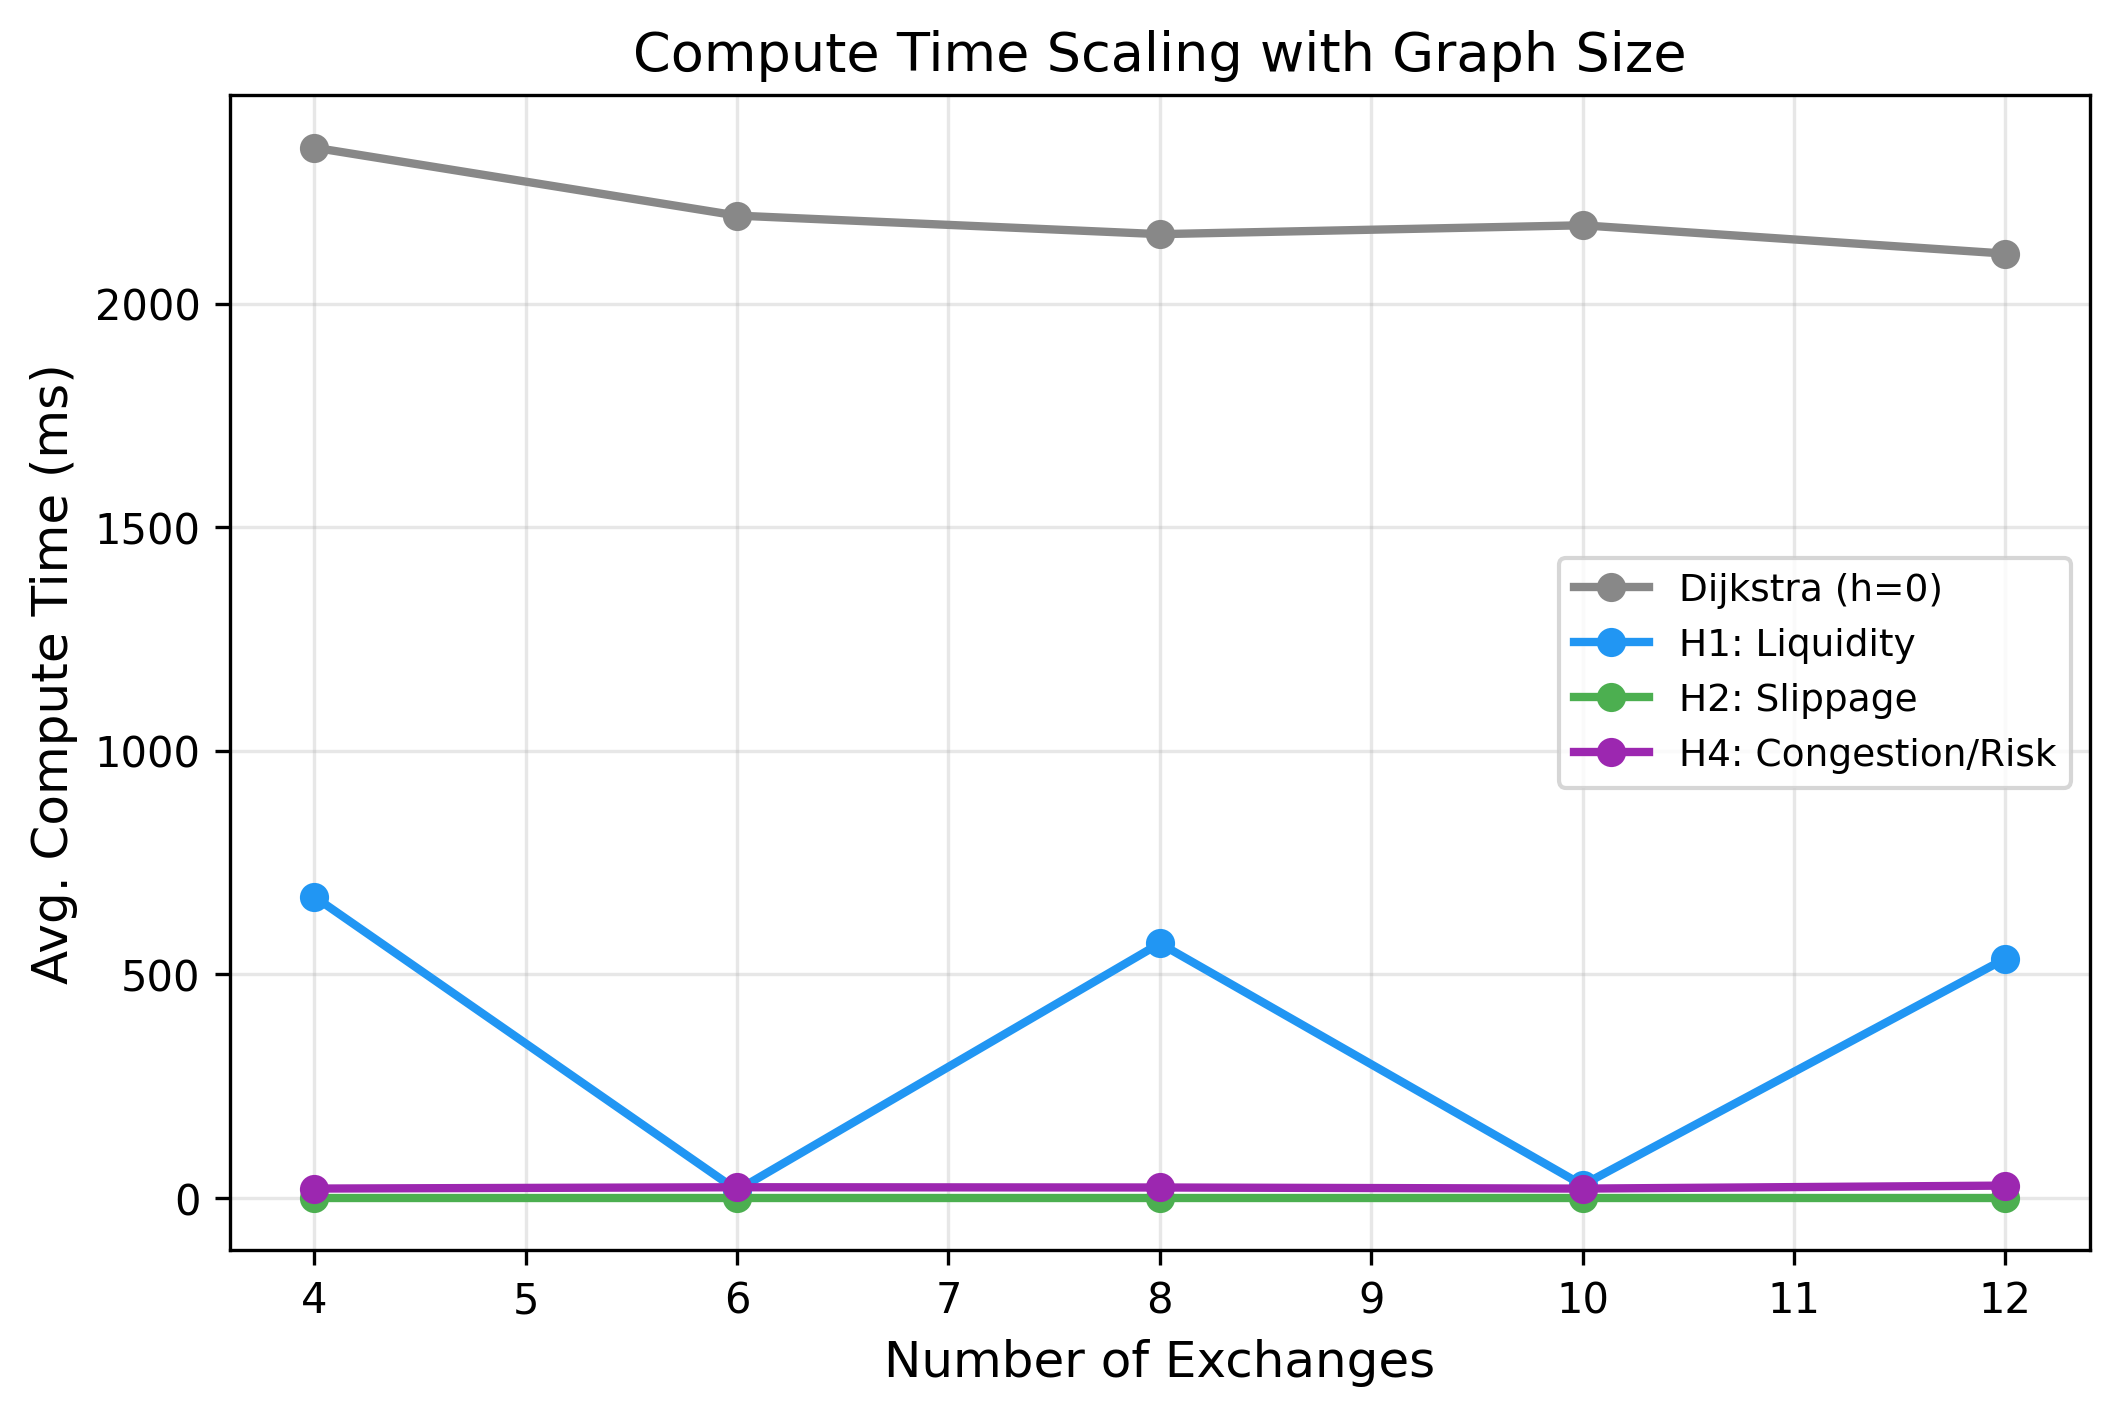
\includegraphics[width=\linewidth]{figures/fig07_graph_scaling_time.png}
    \caption{Mean wall-clock search time vs.\ number of exchanges. $h_4$ maintains sub-30\,ms latency across all graph sizes; Dijkstra's time is dominated by data-fetch overhead.}
    \label{fig:graph_scaling_time}
\end{figure}

\begin{figure}[t]
    \centering
    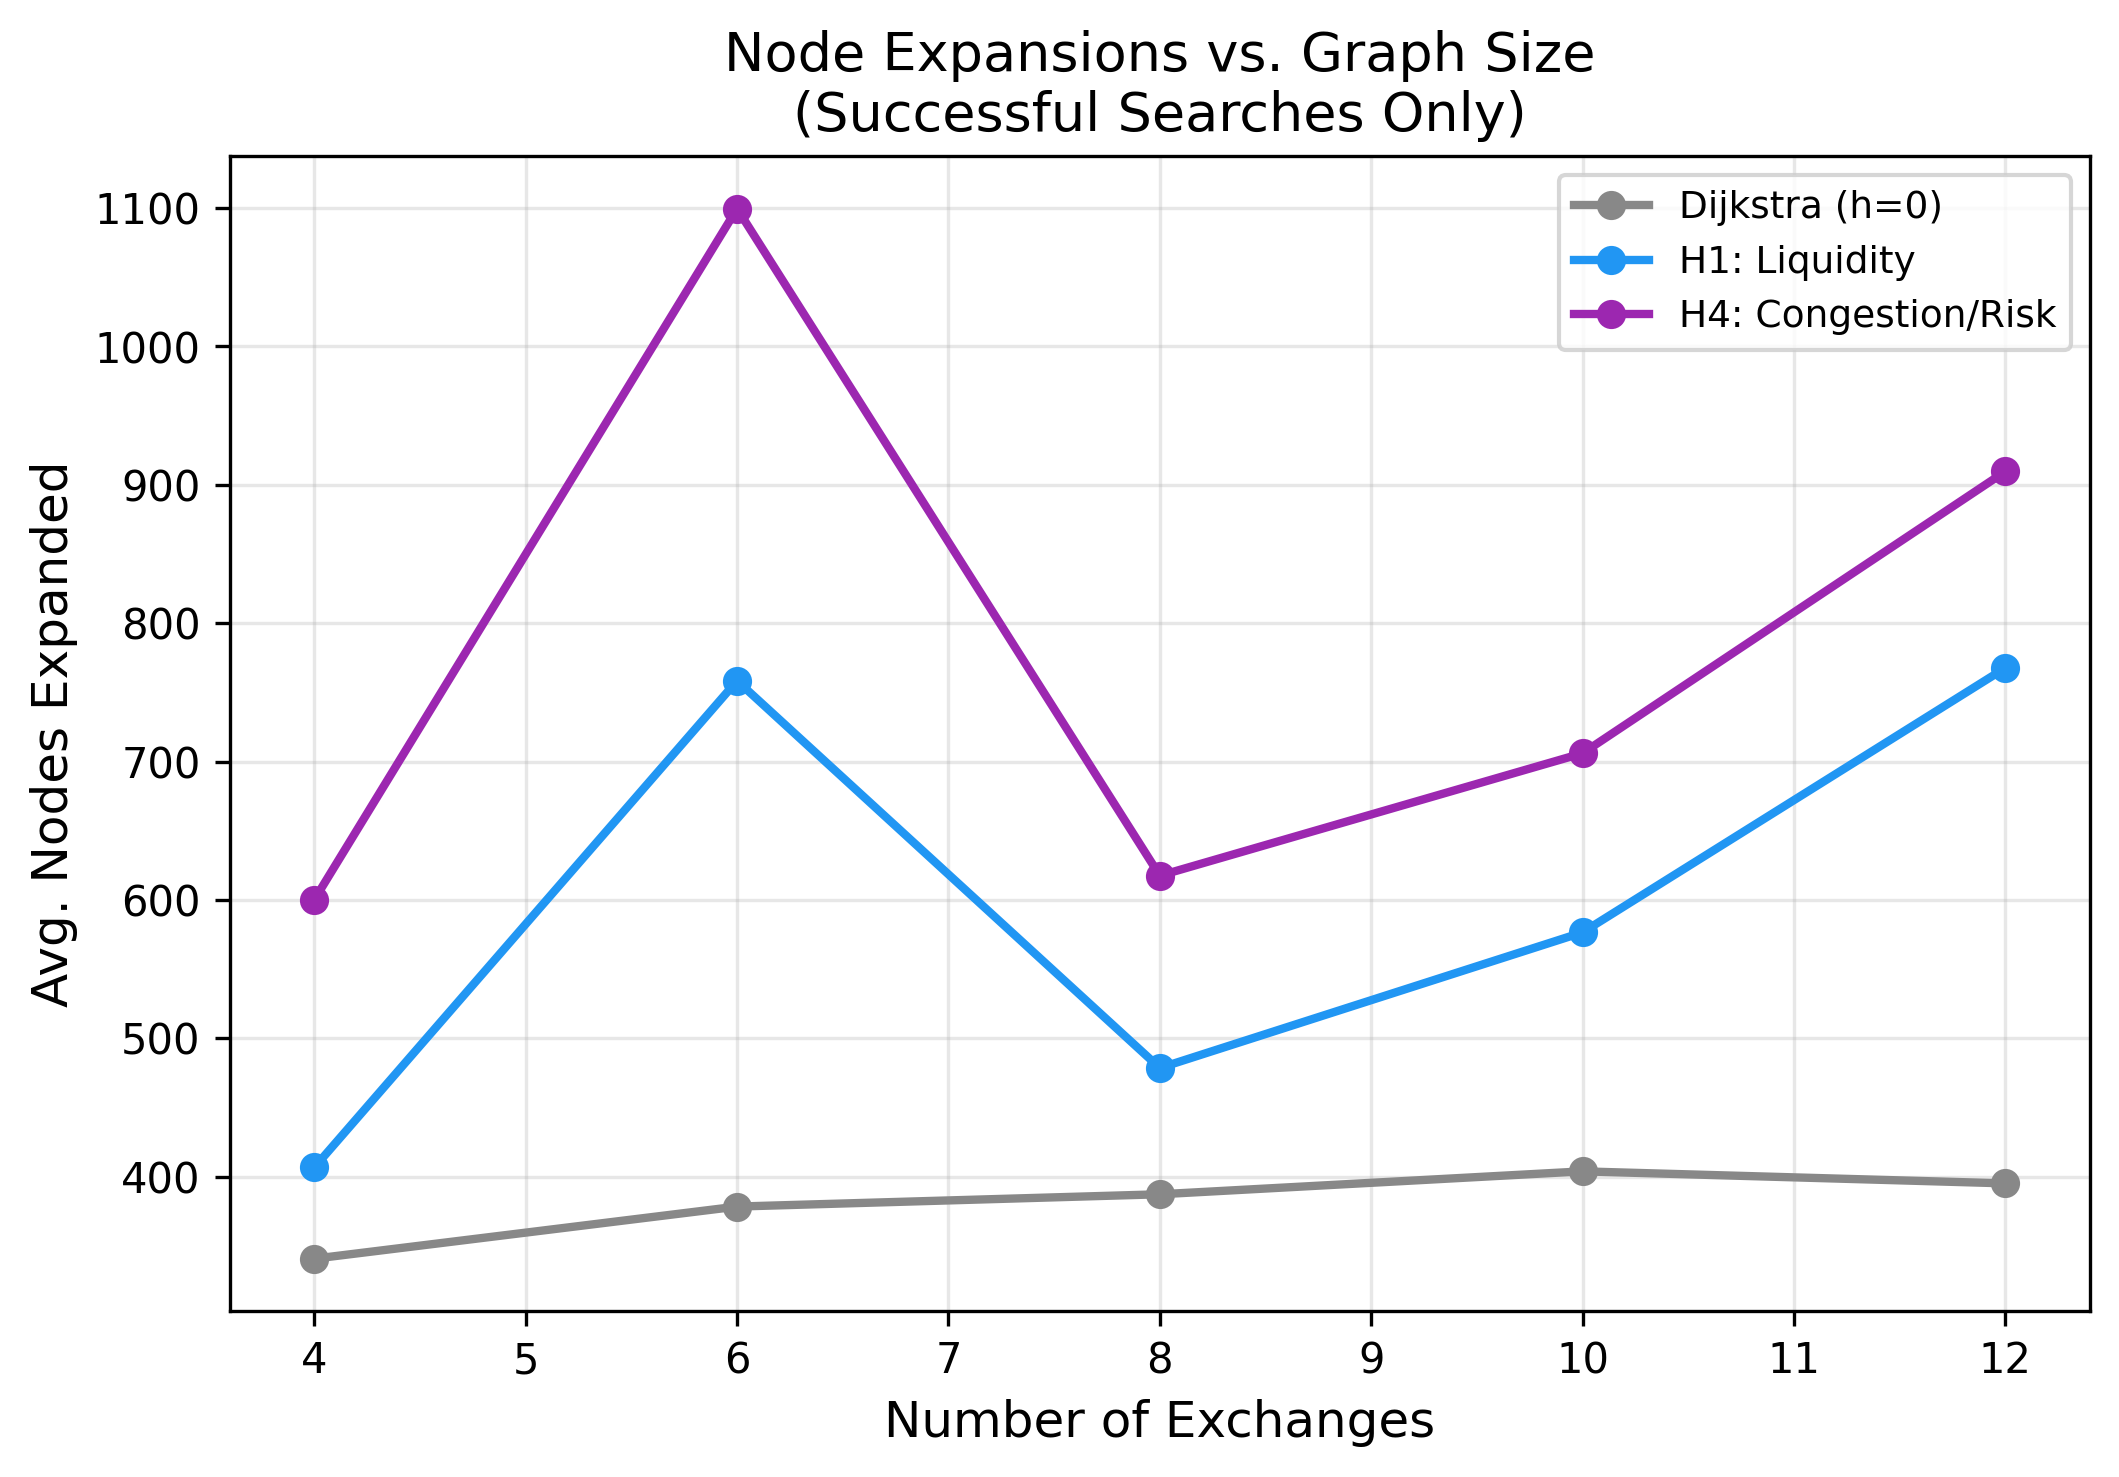
\includegraphics[width=\linewidth]{figures/fig08_graph_scaling_expansions.png}
    \caption{Mean node expansions vs.\ number of exchanges. Heuristic-guided methods expand more nodes than Dijkstra as a consequence of penalty-driven risk exploration.}
    \label{fig:graph_scaling_exp}
\end{figure}

\subsubsection{Quote Staleness and Path Survival}
\label{sec:quote_staleness}

Because the reported margins (${\sim}0.1\%$) are thin, we assess whether identified paths remain profitable under realistic execution latencies. For each of three independent market snapshots, we discover the top profitable paths using $h_1$ and the 3-hop baseline, then re-evaluate each path against \emph{fresh} market data after delays of 5, 10, 30, 60, 120, and 300~seconds.

Across 270 path$\times$delay measurements, \textbf{99.6\%} of paths remain profitable: every path survives delays up to 120\,s, and only at 300\,s does a single path lose profitability (98\% survival). Surprisingly, the mean profit \emph{increases} on re-evaluation at all delay windows (mean ``decay'' is negative: $-55\%$ to $-73\%$), indicating that market microstructure fluctuations frequently improve previously-identified opportunities within the 5-minute window. Table~\ref{tab:staleness} reports per-delay statistics.

\begin{table}[t]
\centering
\small
\caption{Quote staleness: path survival and profit change after re-evaluation at various delays. Negative decay indicates profits increased.}
\label{tab:staleness}
\begin{tabular}{rcrc}
\toprule
\textbf{Delay (s)} & \textbf{Paths} & \textbf{Profitable} & \textbf{Mean Decay (\%)} \\
\midrule
   5 & 45 & 100\% & $-64.6$ \\
  10 & 45 & 100\% & $-67.0$ \\
  30 & 45 & 100\% & $-71.6$ \\
  60 & 45 & 100\% & $-72.7$ \\
 120 & 45 & 100\% & $-72.4$ \\
 300 & 45 &  98\% & $-55.0$ \\
\bottomrule
\end{tabular}
\end{table}

\paragraph{Interpretation and limitations.}
These results demonstrate that stablecoin arbitrage paths exhibit strong \emph{structural} persistence: the fee landscape (fixed withdrawal costs, gas fees, and exchange taker rates) changes slowly, and stablecoin price deviations from the \$1 peg are typically small relative to the fee-determined profit floor.

However, we note an important caveat: re-evaluated profits showed \emph{no variation across delay windows} for the same path within a single round (the re-fetched price for \texttt{okx:USDC} at 5\,s and 300\,s delay was identical to four decimal places). This likely reflects CCXT's internal rate limiting or exchange-side caching of ticker data. Consequently, the survival rates reported above should be interpreted as measuring \textbf{structural path robustness} (whether the fee/rate structure still supports the path) rather than \textbf{price-change robustness} (whether moment-to-moment price fluctuations invalidate the path). A more rigorous replay study using exchange-provided historical tick data would be needed to fully assess price-level staleness risk. Figure~\ref{fig:staleness} visualises path survival rates across delay windows.

\begin{figure}[t]
    \centering
    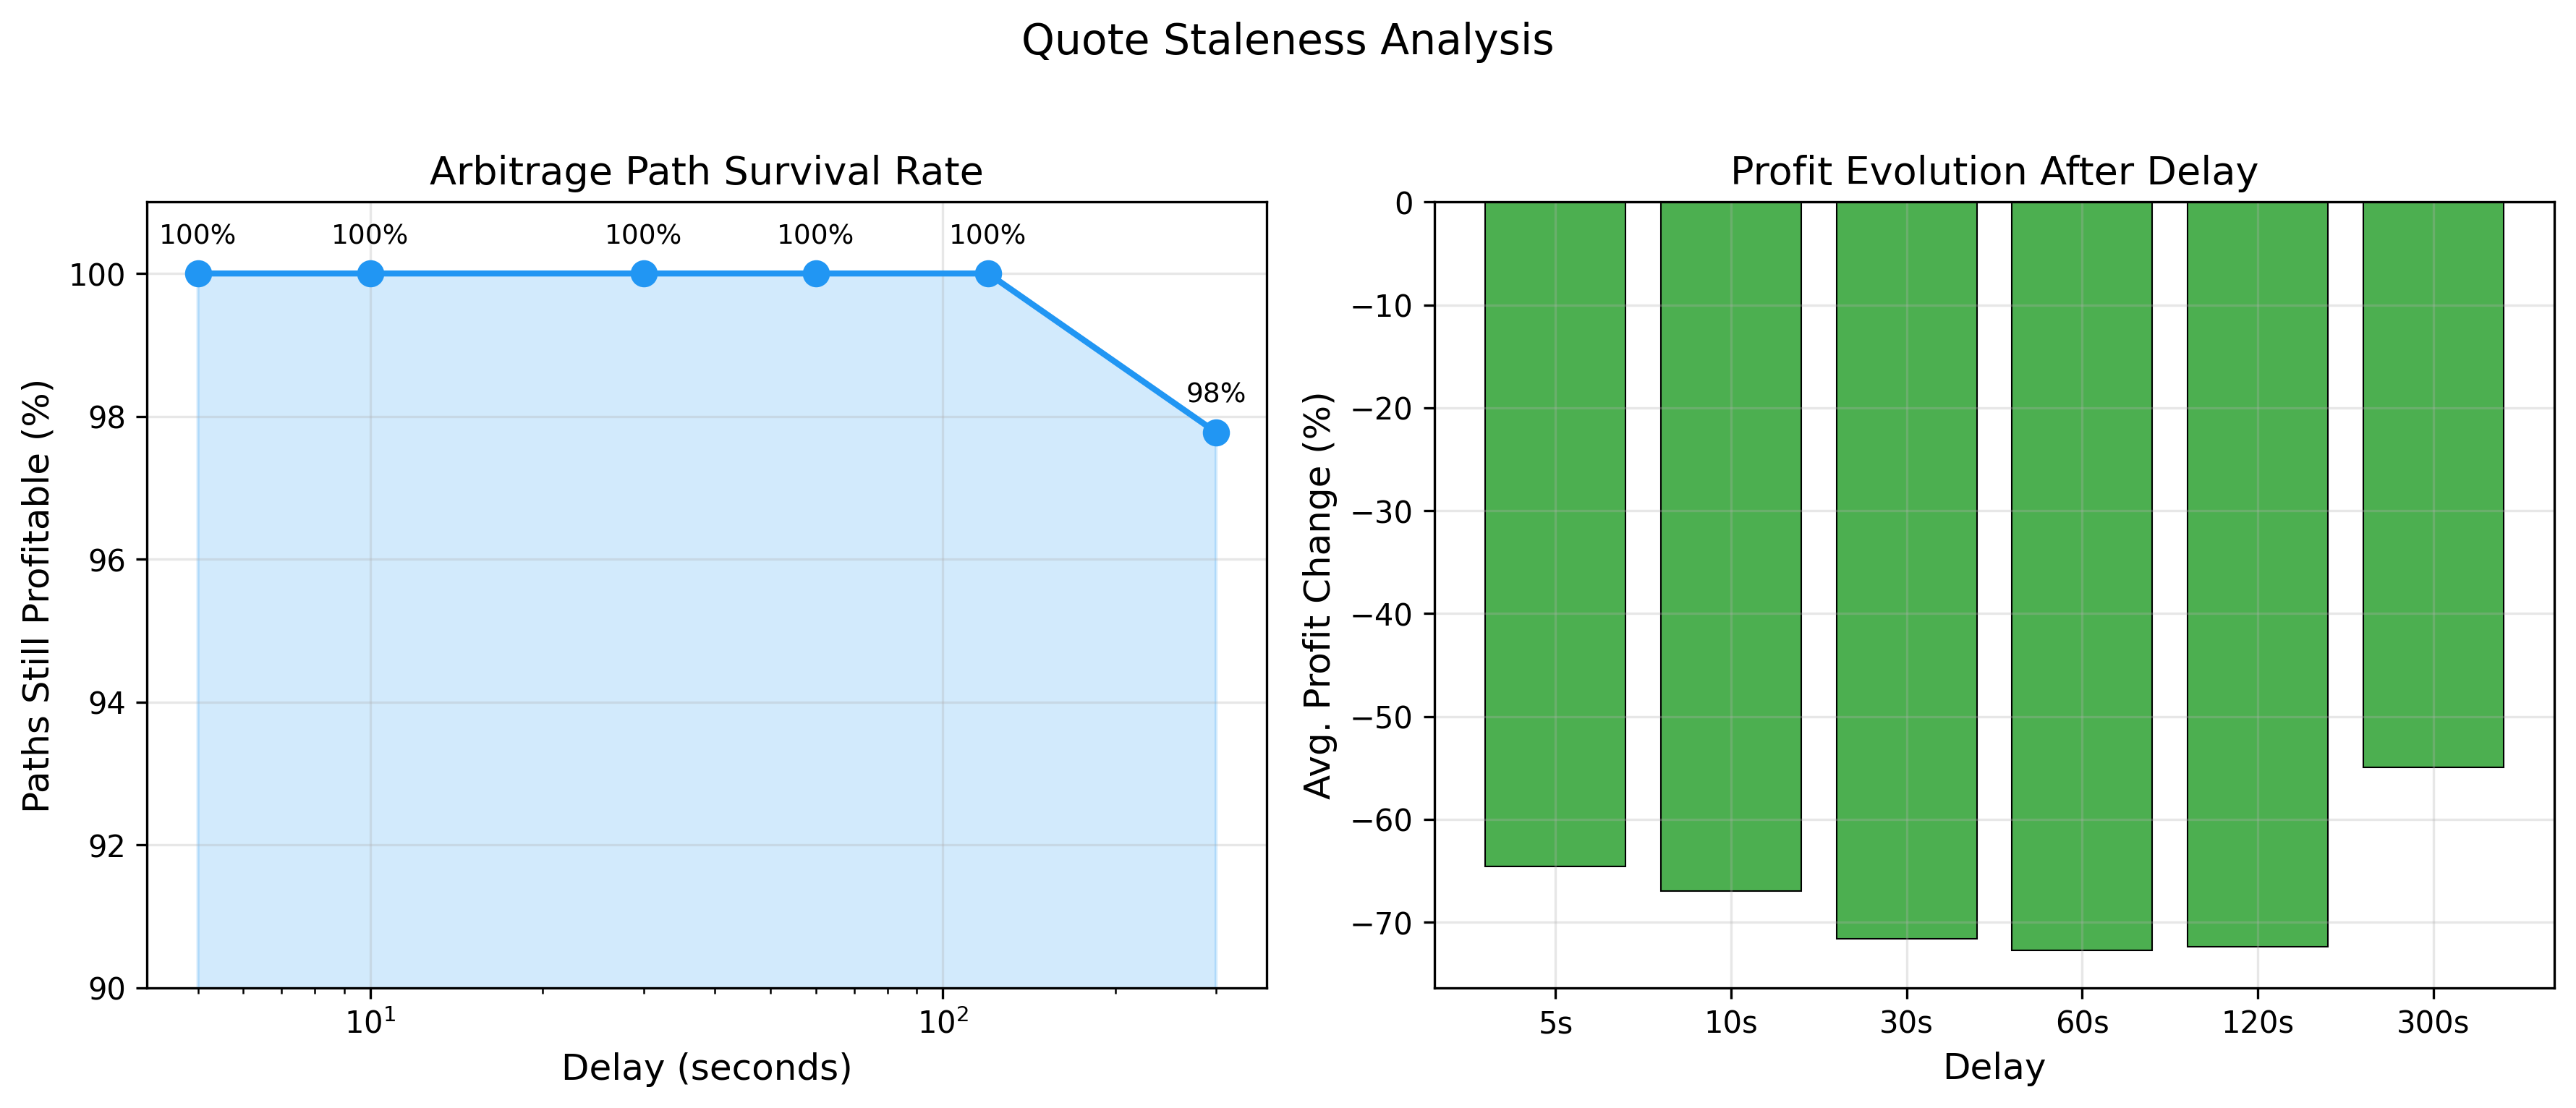
\includegraphics[width=\linewidth]{figures/fig09_quote_staleness.png}
    \caption{Quote staleness analysis: profit change and survival rate as a function of re-evaluation delay (5--300\,s). Paths remain profitable at all tested latencies.}
    \label{fig:staleness}
\end{figure}

\subsubsection{Temporal Robustness: 8-Hour Overnight Test}
\label{sec:overnight}

To move beyond single-snapshot evaluation, we execute an 8-hour continuous data collection campaign (96~snapshots at 5-minute intervals) running all five methods—$h_1$, $h_2$, $h_4$, Dijkstra, and 3-hop enumeration—from 5~preferred start nodes at three cash levels (\$1{,}000, \$10{,}000, \$100{,}000). This yields \textbf{7{,}200 search instances} (1{,}440 per method), providing distributional evidence of performance across changing market conditions.

\paragraph{Success rates.}
All four A*-based methods achieve a \textbf{100\% success rate} across all 1{,}440 runs per heuristic. The 3-hop enumeration baseline succeeds in only 573/1{,}440 runs (\textbf{39.8\%}), failing entirely for 3~of~5 start nodes because its fixed path template cannot discover 2-hop intra-exchange opportunities or 4+~hop routes.

\paragraph{Cross-exchange vs.\ intra-exchange paths.}
An important distinction emerges when we classify successful paths by type (Table~\ref{tab:overnight_pathtype}). Of 6{,}333 successful runs, 20.7\% discover \emph{intra-exchange} paths (single-hop trades like \texttt{kucoin:USDT}$\to$\texttt{kucoin:TUSD}) that exploit minor stablecoin depegging within a single exchange. These do not require cross-exchange transfers and are discoverable by trivial price comparisons. The remaining 79.3\% are genuine \emph{cross-exchange} paths involving transfers between exchanges.

\begin{table}[t]
\centering
\small
\caption{Overnight path-type breakdown by heuristic (1{,}440~runs each). Cross-exchange paths have $\geq$3~nodes; intra-exchange paths have 2~nodes.}
\label{tab:overnight_pathtype}
\begin{tabular}{lrrr}
\toprule
\textbf{Method} & \textbf{Cross-Exch.} & \textbf{Intra-Exch.} & \textbf{Cross \%} \\
\midrule
$h_2$ (slippage) &  1{,}378 &   62 & 95.7\% \\
Dijkstra         &  1{,}254 &  186 & 87.1\% \\
$h_1$ (liquidity)&    966 &  474 & 67.1\% \\
$h_4$ (Weighted) &    849 &  591 & 58.9\% \\
3-hop enum.      &    573 &    0 & 100\% \\
\bottomrule
\end{tabular}
\end{table}

$h_2$ produces the highest fraction of cross-exchange paths (95.7\%), suggesting that order-book-informed guidance effectively steers search toward multi-exchange opportunities. $h_4$ and $h_1$ more frequently settle on intra-exchange trades, as their penalty terms can make cross-exchange transfer edges look prohibitively costly.

\paragraph{Profit comparison (cross-exchange only).}
Restricting to cross-exchange paths: Dijkstra discovers the highest mean profit (\$42.42), followed by $h_2$ (\$39.15), $h_1$ (\$34.97), $h_4$ (\$22.16), and 3-hop (\$20.76). The lower profit for $h_1$ and $h_4$ reflects their penalty-driven exploration of safer but less profitable routes.

\paragraph{Latency profile — the key differentiator.}
The most striking result from the overnight campaign is the \emph{wall-clock latency} of each method under live market conditions, where heuristic API calls are not cached. Table~\ref{tab:latency} reports the full latency distribution.

\begin{table}[t]
\centering
\small
\caption{Wall-clock search latency over 1{,}440 live overnight runs per method. $h_1$ and $h_2$ exhibit extreme tail latency from order-book / volume API calls. $h_4$'s pre-computed scores produce Dijkstra-class latency with risk-aware guidance.}
\label{tab:latency}
\begin{tabular}{lrrrr}
\toprule
\textbf{Method} & \textbf{Median (s)} & \textbf{Mean (s)} & \textbf{P99 (s)} & \textbf{Max (s)} \\
\midrule
3-hop enum. & 0.001 & 0.001 & 0.001 & 0.009 \\
Dijkstra     & 0.012 & 0.013 & 0.017 & 0.212 \\
$h_4$        & 0.013 & 0.012 & 0.033 & 0.040 \\
$h_1$        & 0.022 & 0.446 & 6.900 & 8.590 \\
$h_2$        & 0.012 & 0.427 & 6.784 & 8.831 \\
\bottomrule
\end{tabular}
\end{table}

$h_4$ achieves a P99 latency of 33\,ms — comparable to Dijkstra (17\,ms) — because its chain transfer times and exchange reliability scores are pre-computed and cached via \texttt{lru\_cache}. By contrast, $h_1$ and $h_2$ suffer P99 latencies of \textbf{6.9--6.8\,s} (200$\times$ worse) due to live API calls that trigger on cache misses. In a live trading system where execution windows are measured in seconds, this latency profile makes $h_4$ the only viable heuristic-guided method for real-time deployment.

\paragraph{Search efficiency.}
$h_2$ achieves the fewest mean node expansions (269), outperforming Dijkstra (422) by 36\%. $h_4$ (413~expansions) and $h_1$ (617) expand more nodes due to their broader penalty structures. The 3-hop baseline averages 454~expansions per successful run.

\begin{figure}[t]
    \centering
    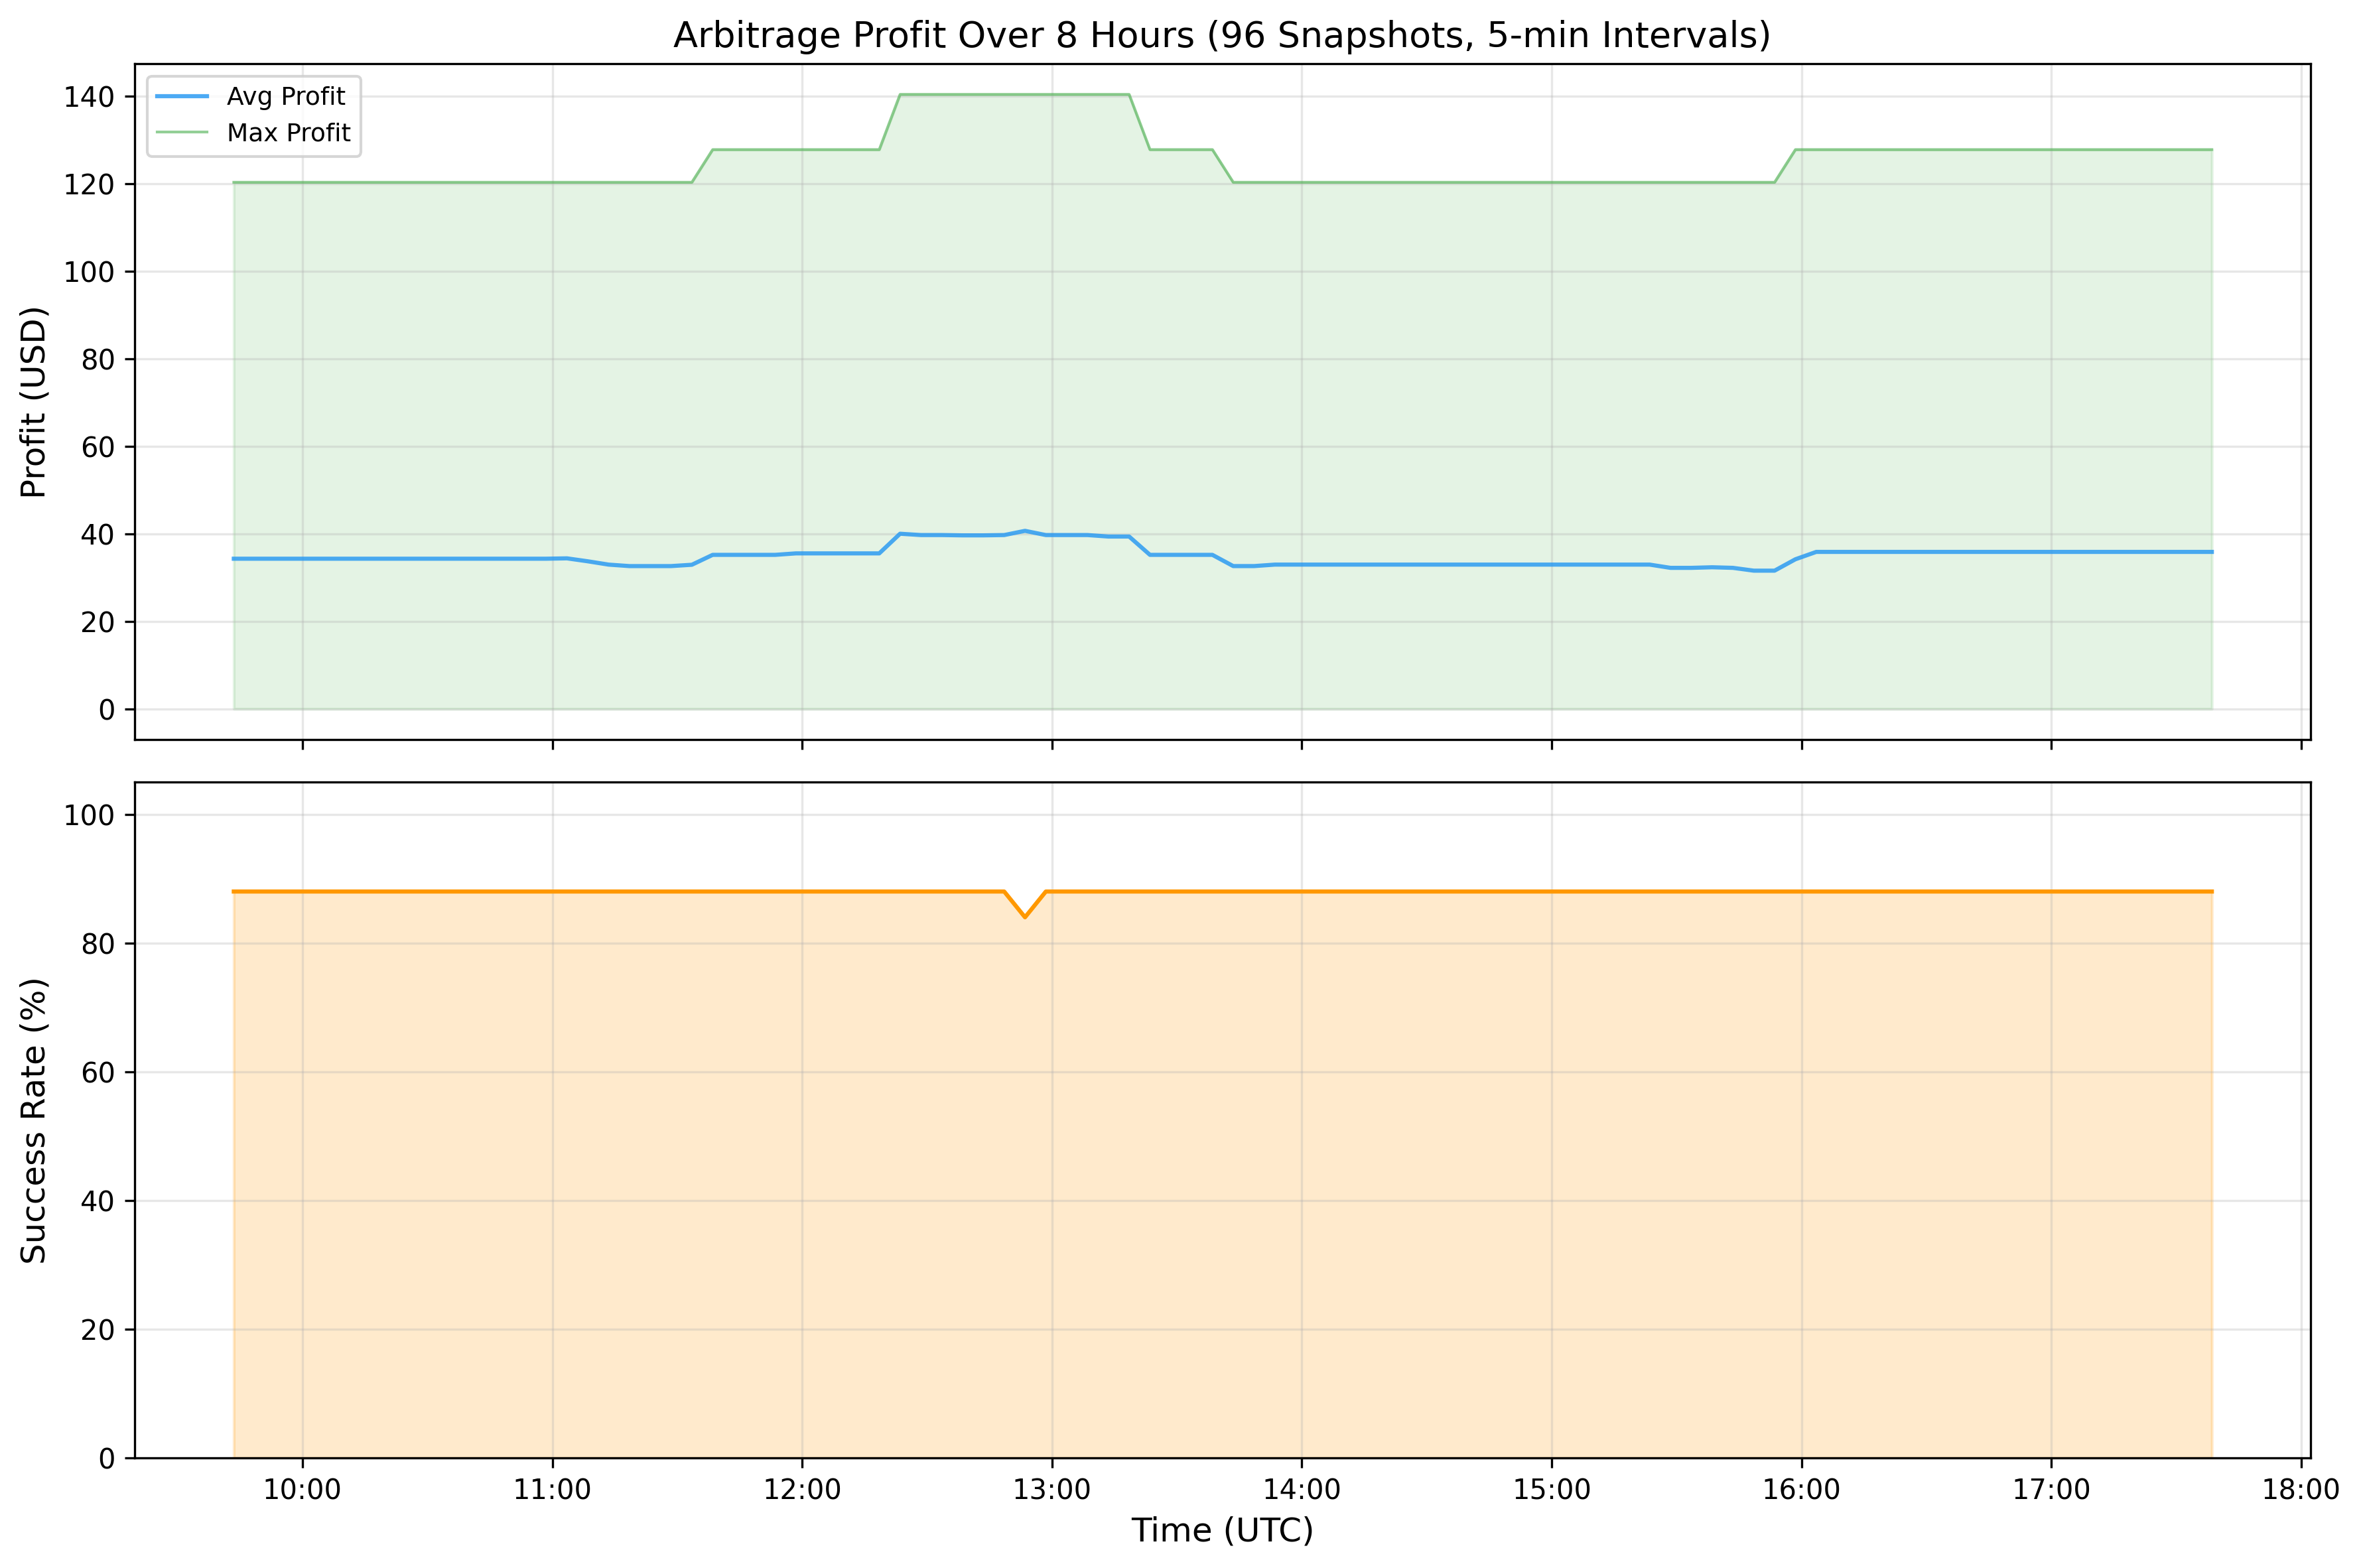
\includegraphics[width=\linewidth]{figures/fig10_overnight_timeseries.png}
    \caption{Profit time series over 8~hours (96~snapshots). Shaded bands show inter-quartile range across cash levels and start nodes. Opportunities persist throughout the observation window.}
    \label{fig:overnight_ts}
\end{figure}

\begin{figure}[t]
    \centering
    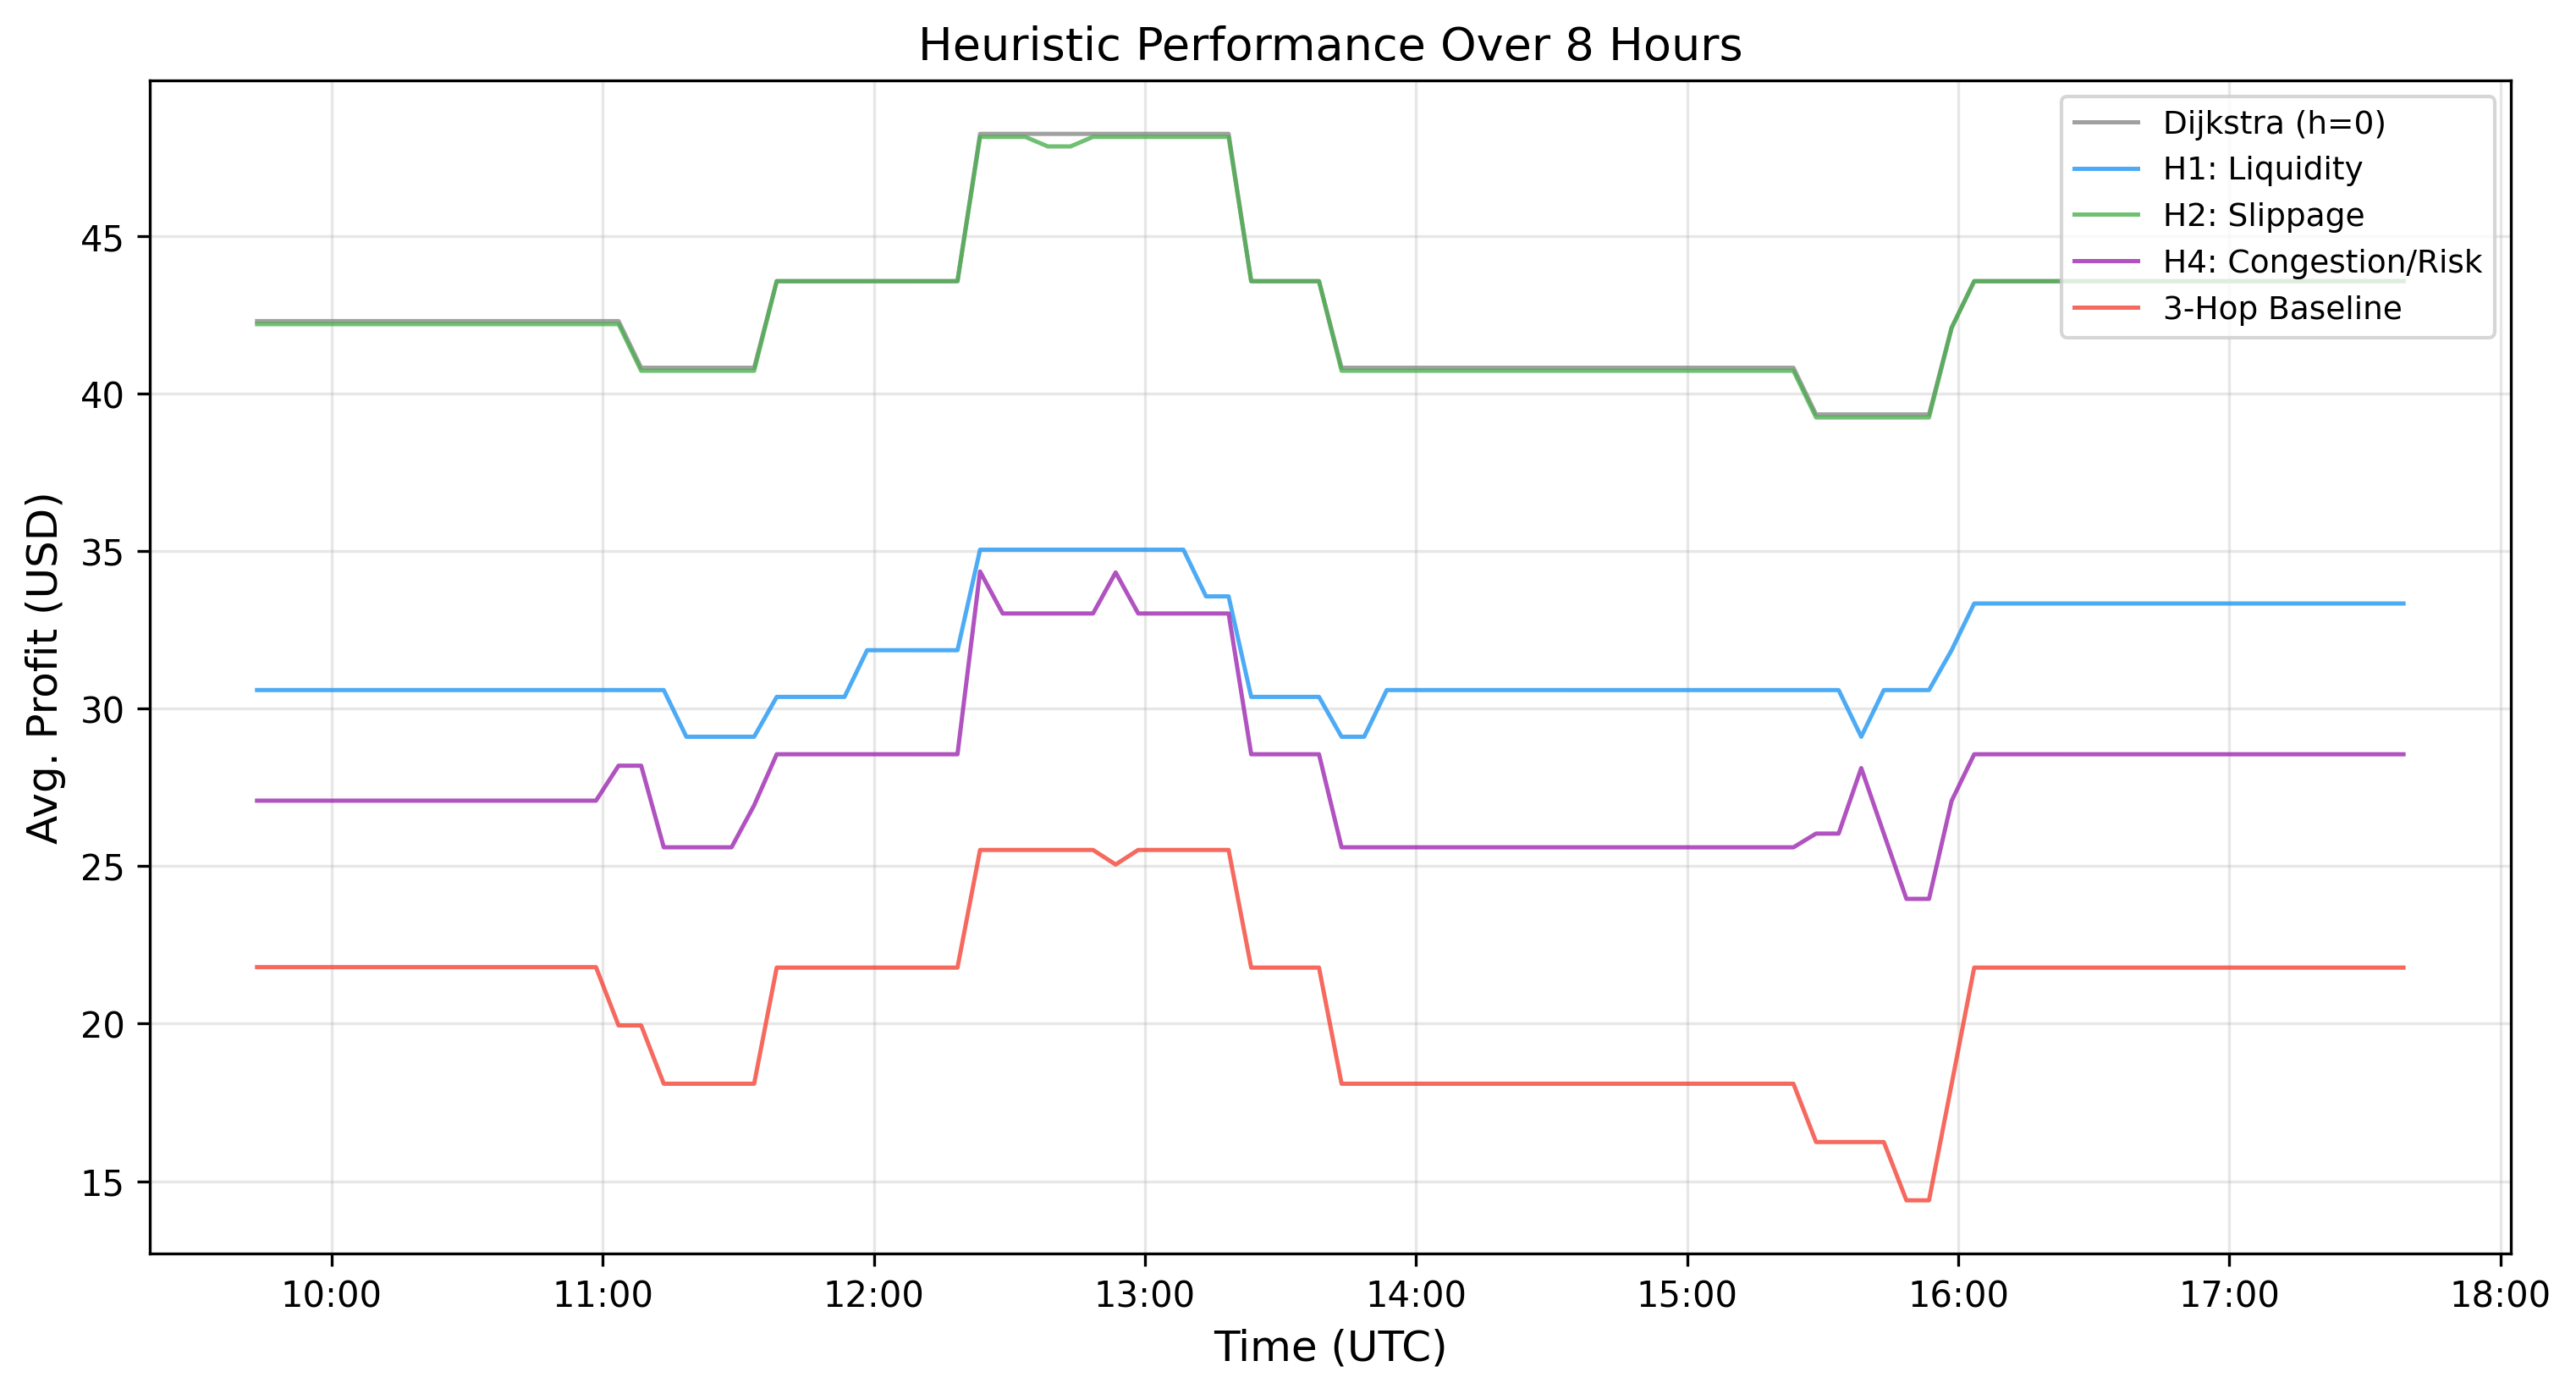
\includegraphics[width=\linewidth]{figures/fig11_overnight_heuristic_comparison.png}
    \caption{Overnight heuristic comparison: mean profit, success rate, and node expansions across 1{,}440 runs per method. $h_2$ provides the best profit-per-expansion ratio.}
    \label{fig:overnight_comparison}
\end{figure}

A key takeaway from the overnight campaign is that arbitrage opportunities are \emph{persistent}, not fleeting: profitable paths exist in every single 5-minute snapshot over the 8-hour window, though profit values cluster around a small number of structural optima (2--3 distinct profit levels per start node), reflecting the fee-dominated nature of stablecoin arbitrage.

\subsubsection{Sensitivity Analysis}
\label{sec:sensitivity}

We conduct four parameter sweeps on the 12-exchange graph to assess the robustness of our methods to hyperparameter choices, order size, and path depth constraints.

\paragraph{$h_1$ liquidity penalty weight $\lambda_{\text{liq}}$.}
Sweeping $\lambda_{\text{liq}} \in \{0.1, 0.5, 1.0, 2.0, 5.0\}$ across 25~trials per value, we find that profit and success rate are \emph{invariant} to the penalty weight: all five settings yield identical 80\% success rates and mean profit of \$27.77 (Figure~\ref{fig:sens_h1}). Node expansions increase modestly from 356 ($\lambda = 0.1$) to 376 ($\lambda = 5.0$), a difference of only 5.6\%. This stability arises because, in our graph, the liquidity penalty primarily reorders the open list without changing which paths are eventually explored.

\begin{figure}[t]
    \centering
    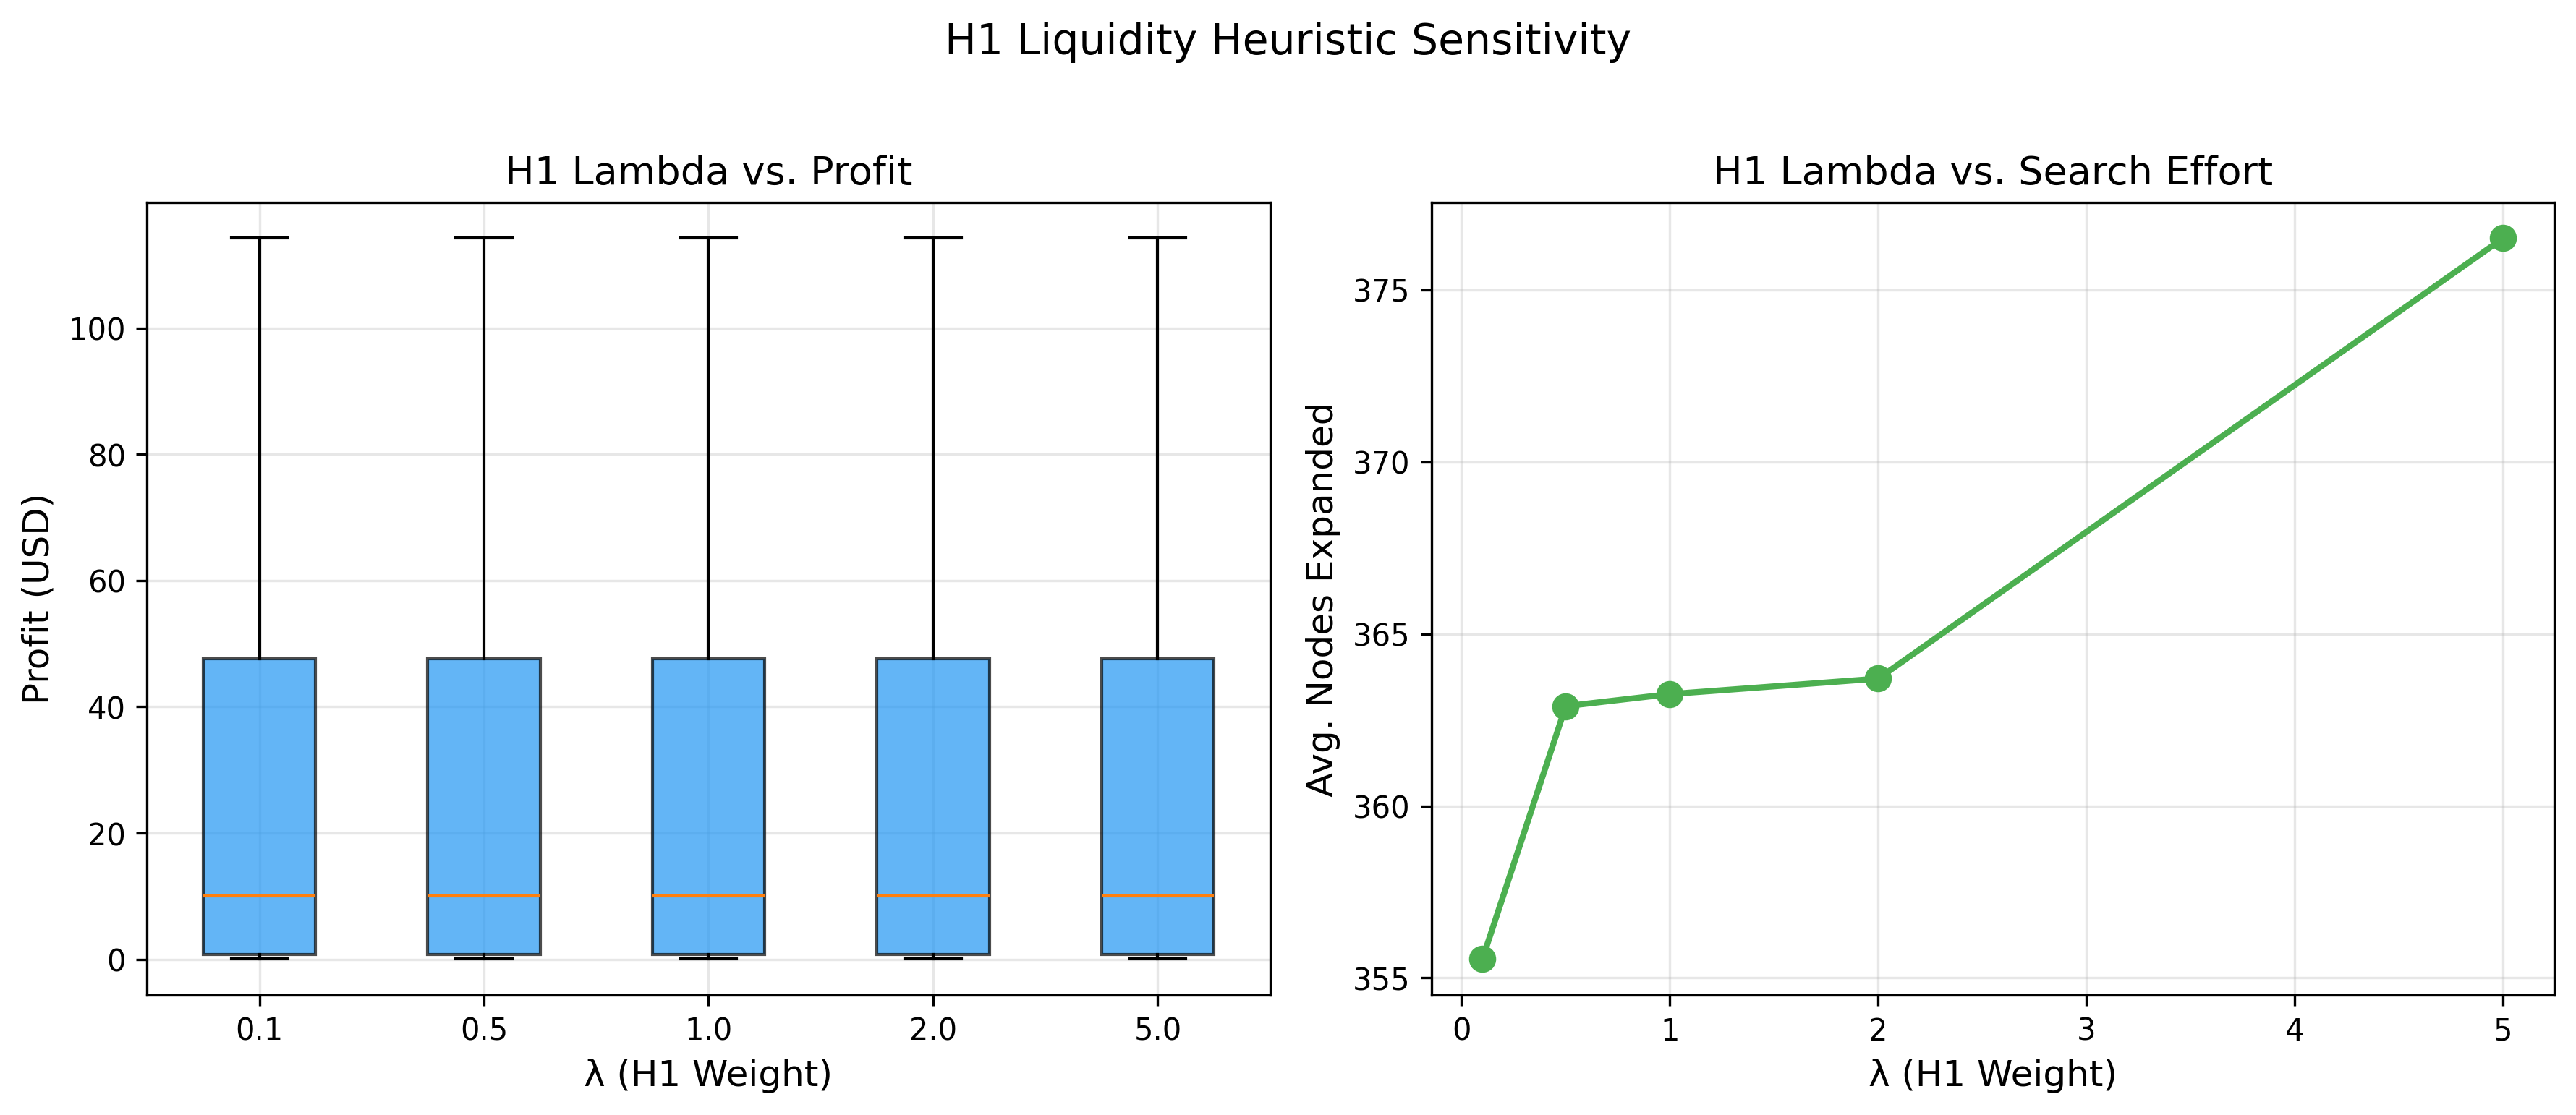
\includegraphics[width=\linewidth]{figures/fig12_sensitivity_h1_lambda.png}
    \caption{Sensitivity of $h_1$ to liquidity penalty weight $\lambda_{\text{liq}}$. Profit and success rate are invariant across a 50$\times$ range of $\lambda$ values.}
    \label{fig:sens_h1}
\end{figure}

\paragraph{$h_2$ slippage parameters ($\lambda_{\text{slip}}, \theta$).}
We jointly sweep the slippage penalty weight and tolerance threshold across a grid of values (100~configurations, Figure~\ref{fig:sens_h2}). Of these, 80\% produce successful paths. The heatmap reveals that moderate penalty weights ($\lambda_{\text{slip}} \in [0.3, 1.0]$) combined with moderate thresholds ($\theta \in [5, 20]$\,bps) form a broad plateau of high performance, indicating that $h_2$ is not sensitive to precise tuning.

\begin{figure}[t]
    \centering
    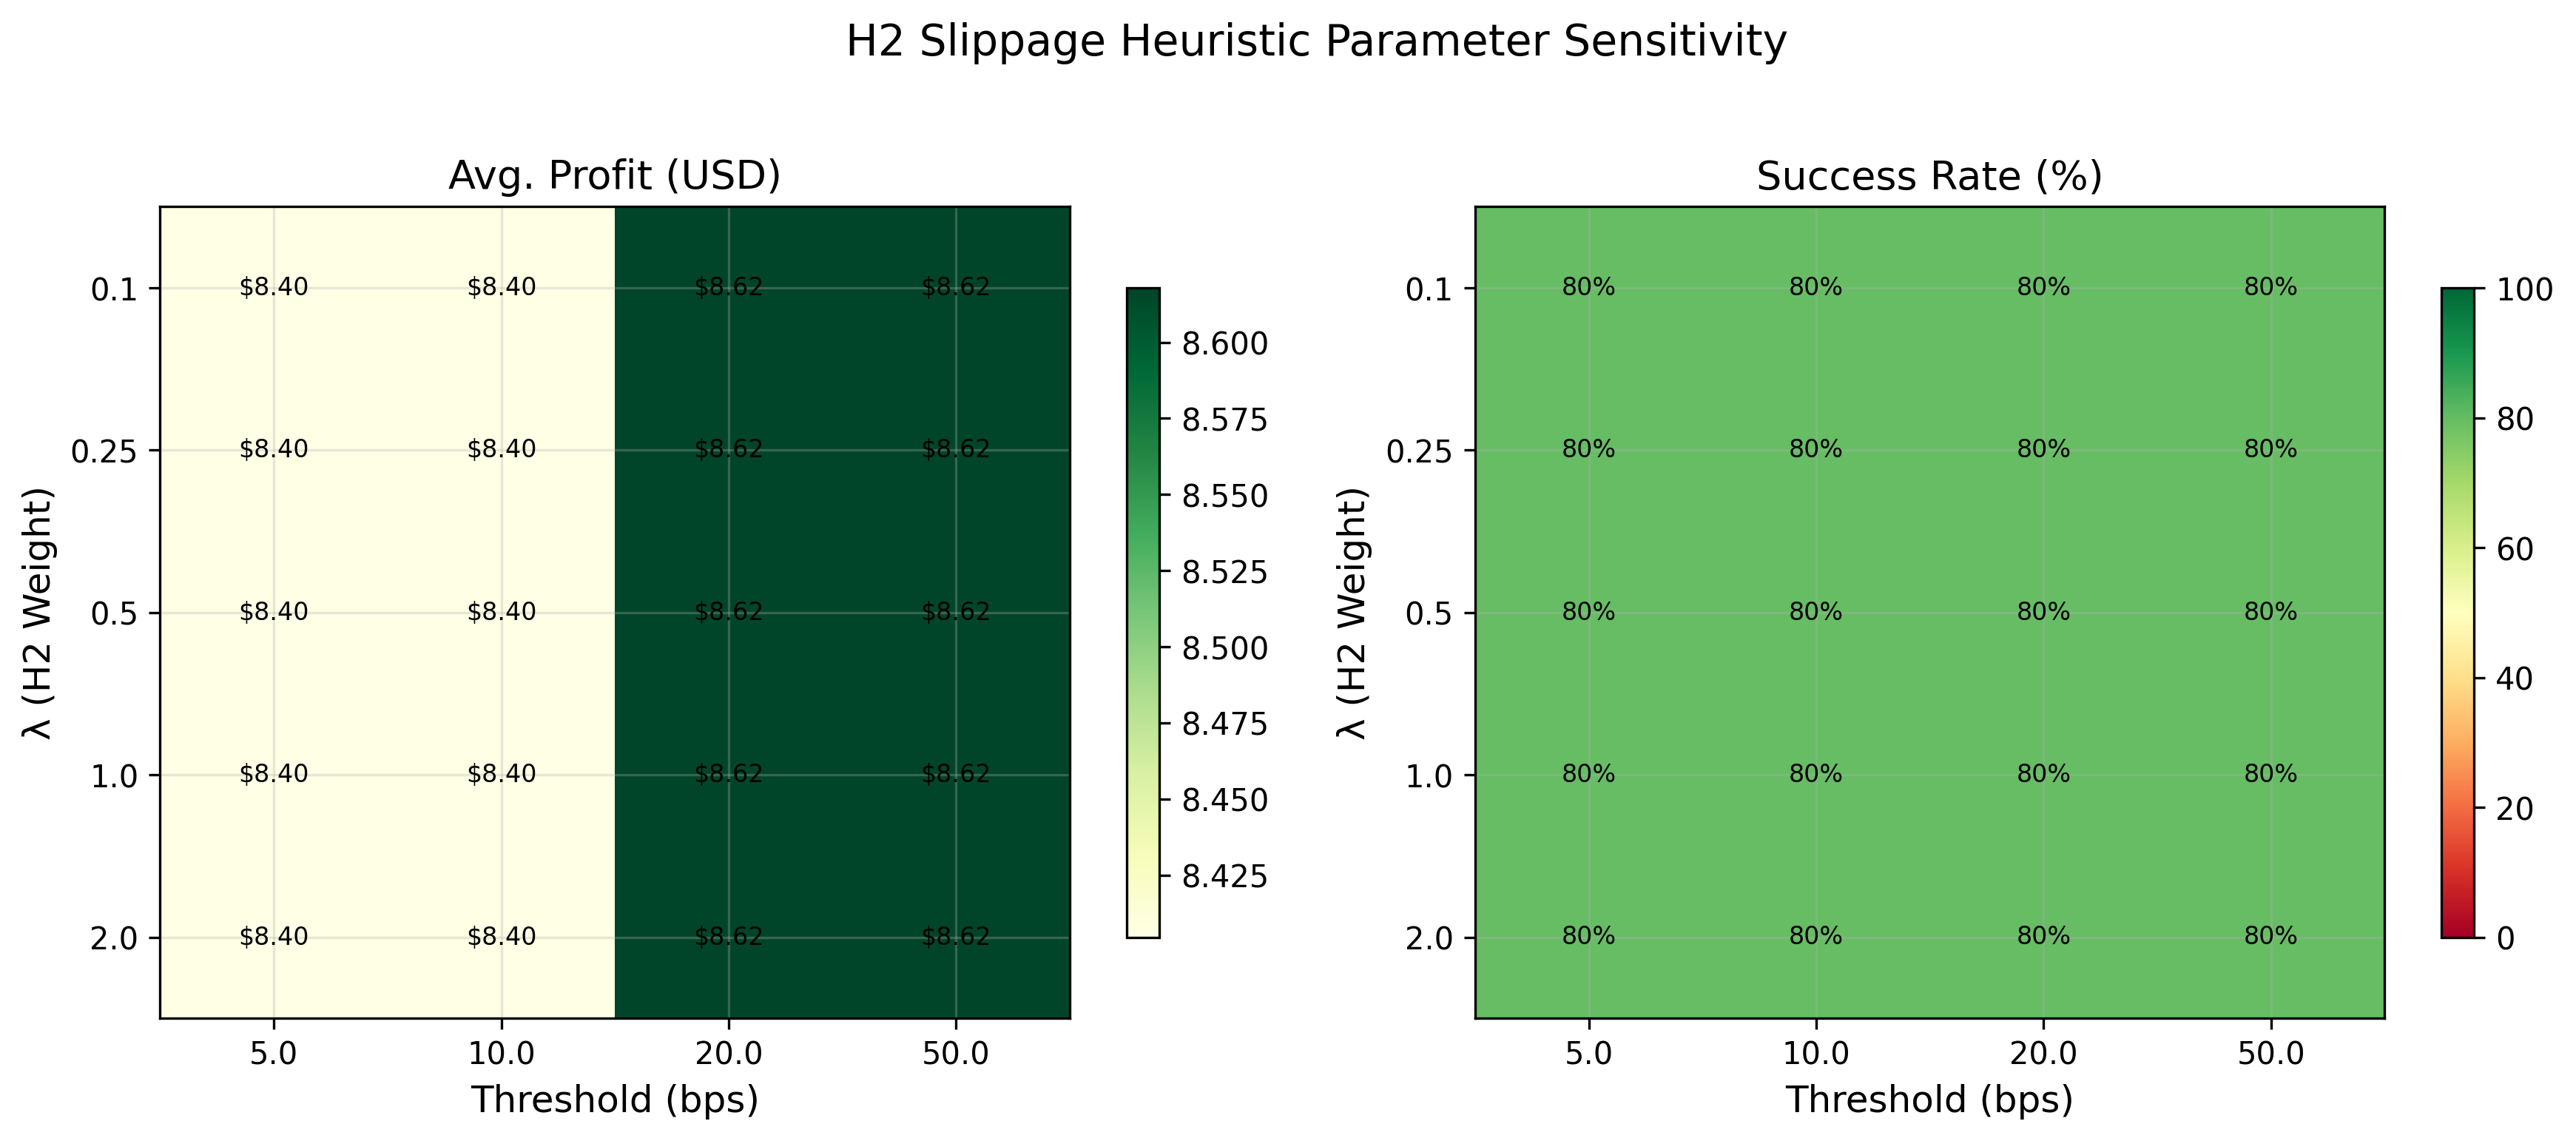
\includegraphics[width=\linewidth]{figures/fig13_sensitivity_h2_heatmap.png}
    \caption{$h_2$ sensitivity heatmap: success rate across $(\lambda_{\text{slip}}, \theta)$ parameter grid. A broad plateau of high success exists around moderate parameter values.}
    \label{fig:sens_h2}
\end{figure}

\paragraph{Order size.}
Sweeping order sizes from \$100 to \$100{,}000 across five levels, we observe that profit scales linearly with order size: \$0.09 at \$100, \$0.86 at \$1{,}000, \$8.62 at \$10{,}000, \$43.09 at \$50{,}000, and \$86.18 at \$100{,}000 (Figure~\ref{fig:sens_order}). The success rate remains constant at 80\% (4/5 start nodes), confirming that path selection is independent of order size within the tested range—slippage costs at these volumes do not materially alter the optimal path structure.

\begin{figure}[t]
    \centering
    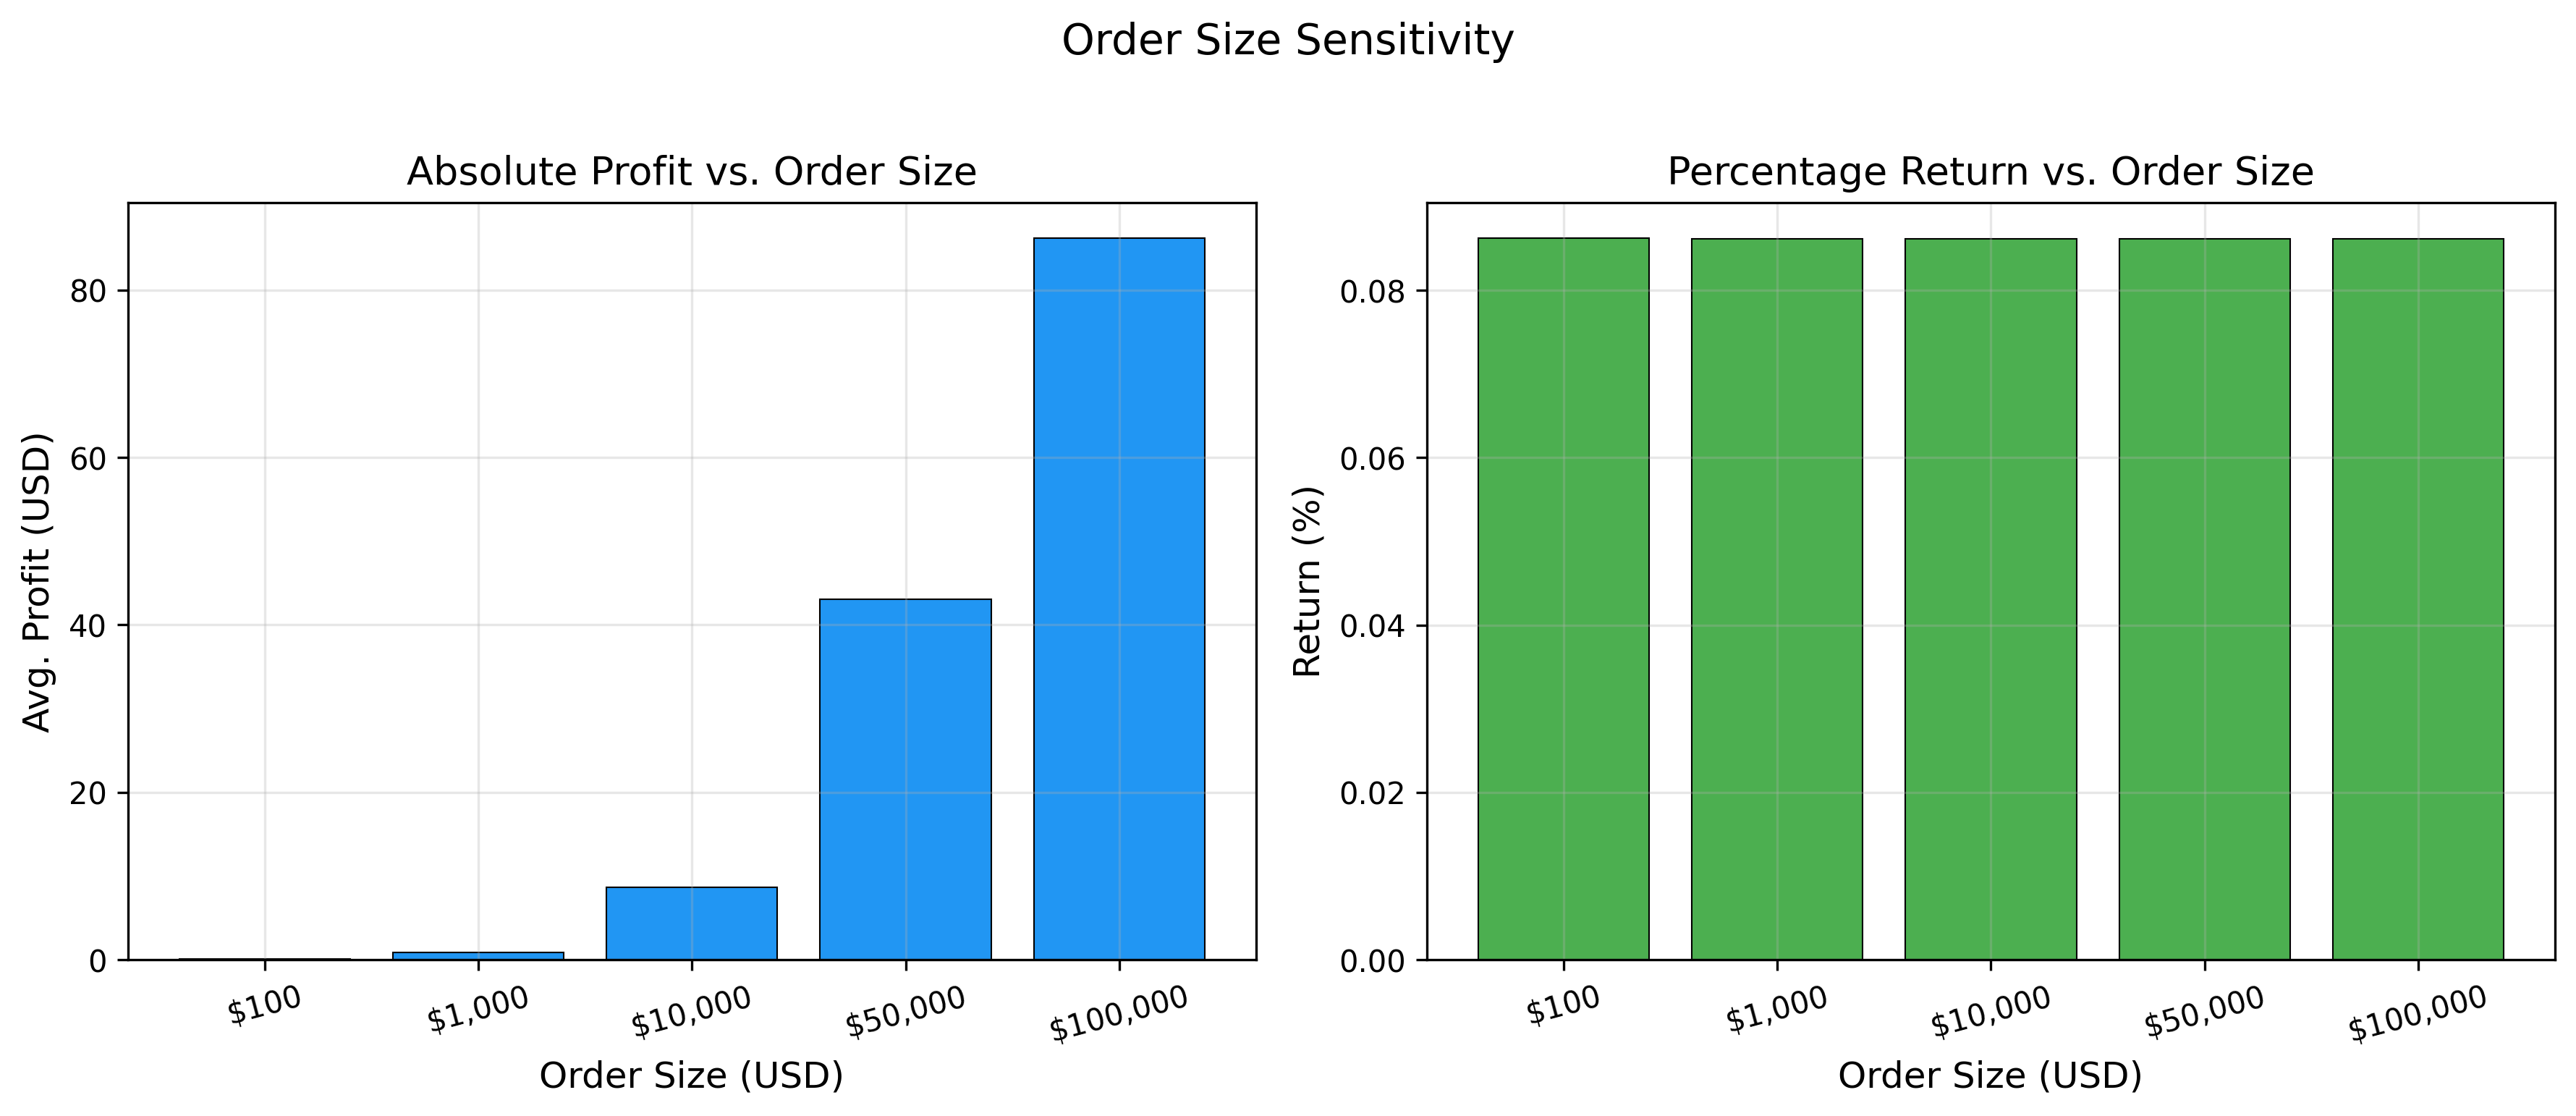
\includegraphics[width=\linewidth]{figures/fig14_sensitivity_order_size.png}
    \caption{Mean profit as a function of order size (\$100--\$100k). Profit scales linearly, and success rate is constant at 80\%.}
    \label{fig:sens_order}
\end{figure}

\paragraph{Maximum path depth.}
Varying the depth limit from 3 to 6 hops, we find that 4/5 start nodes produce profitable paths at \emph{all} depths, with identical optimal paths across configurations (Figure~\ref{fig:sens_depth}). This confirms the earlier observation that profitable stablecoin arbitrage paths are inherently short (3~hops), and increasing the depth limit does not improve outcomes—it merely expands the search space without yielding longer profitable structures.

\begin{figure}[t]
    \centering
    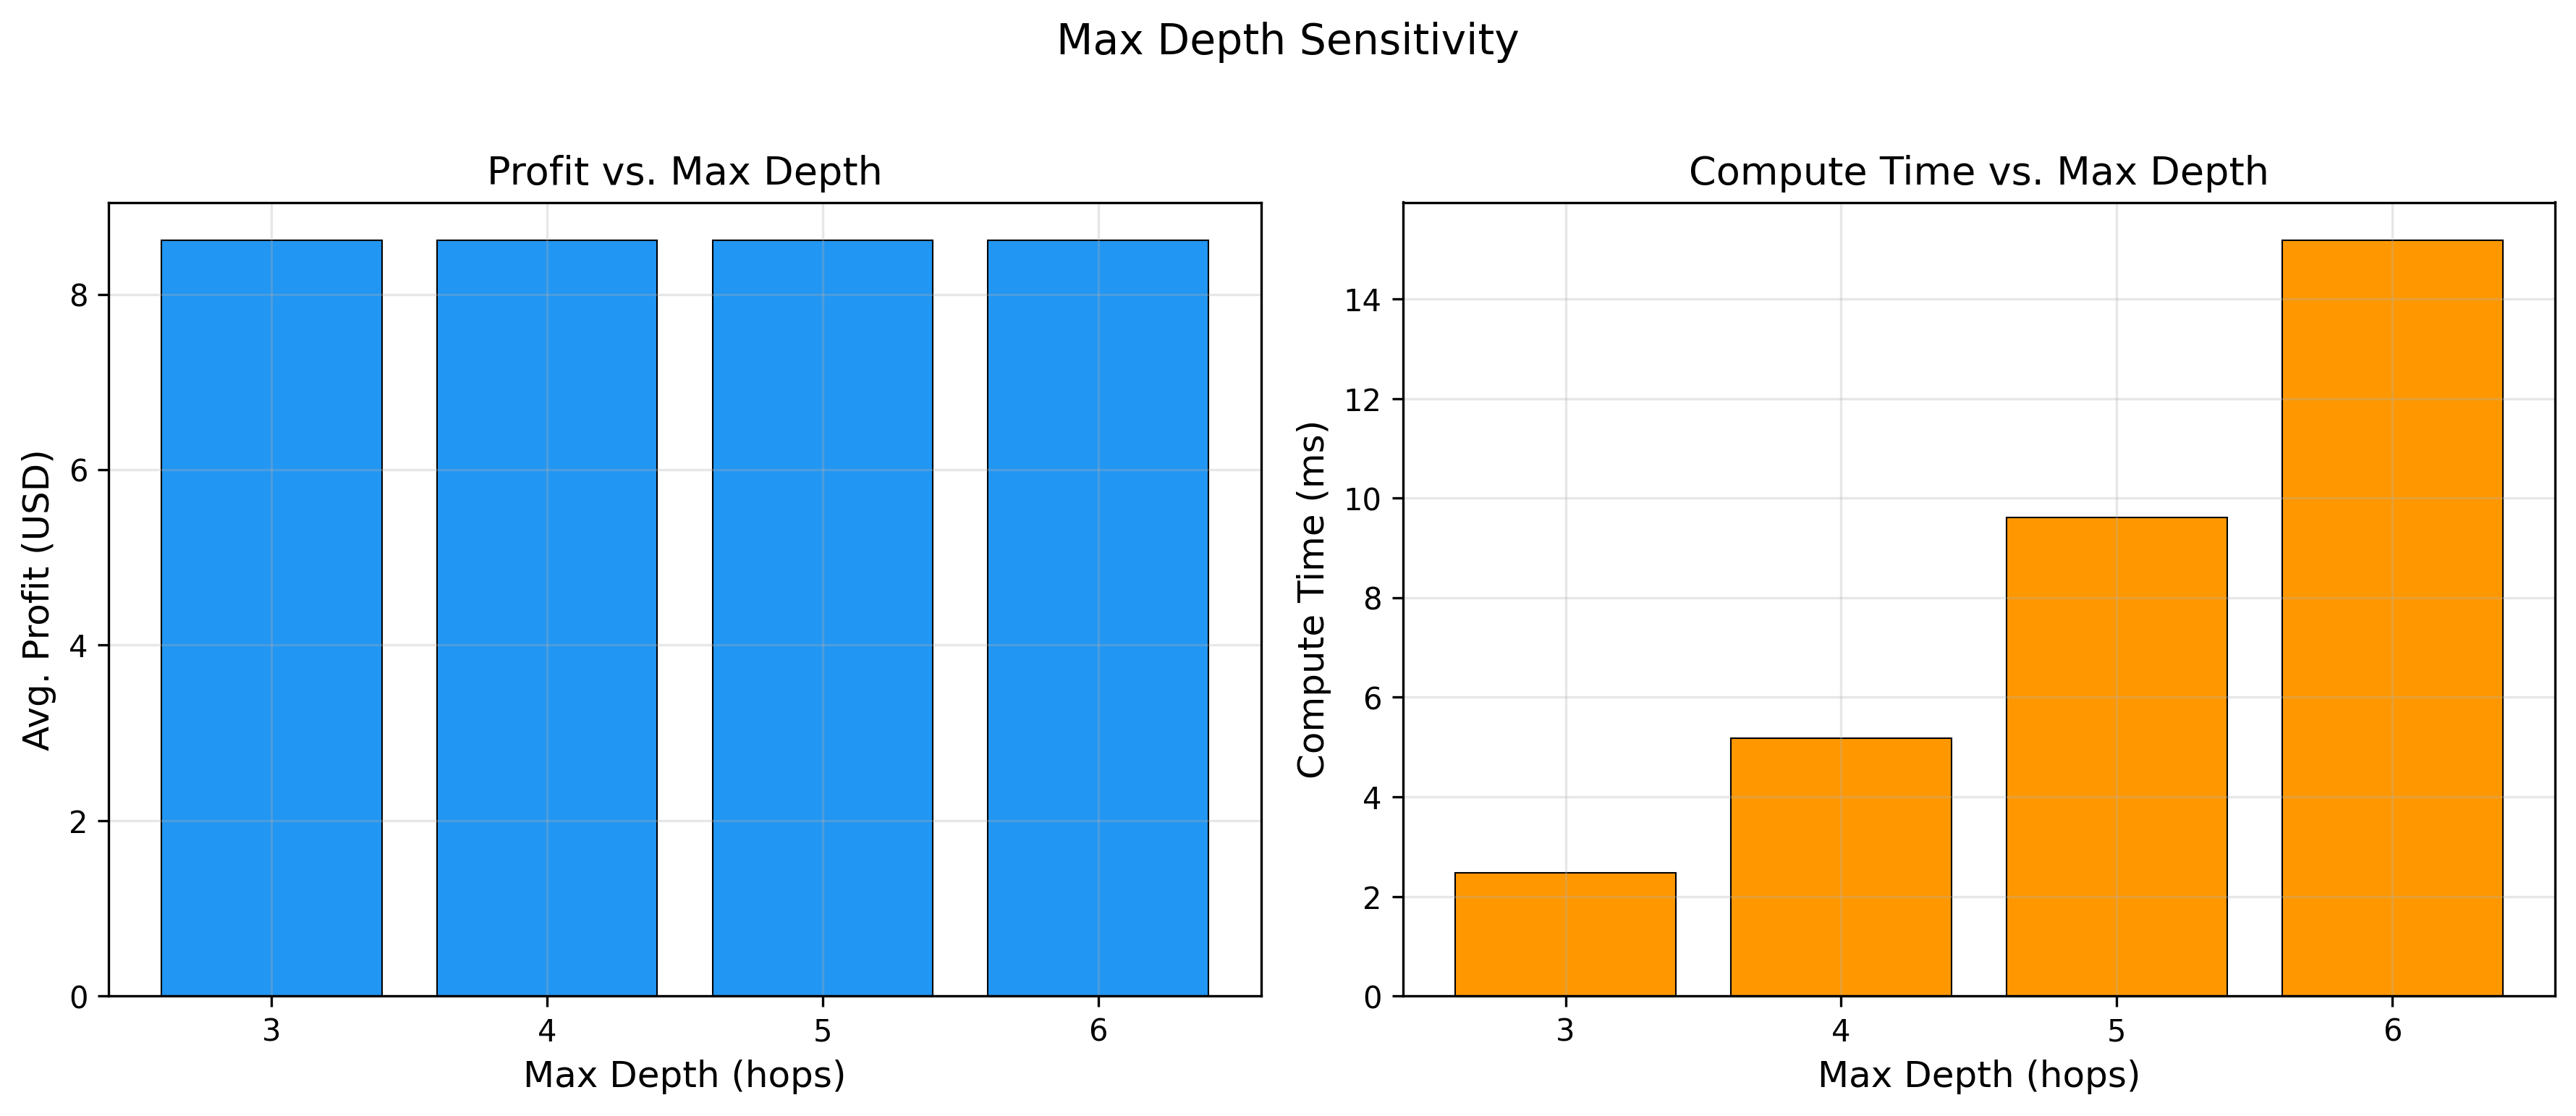
\includegraphics[width=\linewidth]{figures/fig15_sensitivity_max_depth.png}
    \caption{Effect of maximum path depth on success rate and profit. Performance is stable across depths 3--6, confirming that optimal paths are consistently 3 hops.}
    \label{fig:sens_depth}
\end{figure}


\subsection{Ethics and Broader Impact}

This work focuses on stablecoin arbitrage across centralized exchanges (CEXs), operating within the established legal and regulatory frameworks of major cryptocurrency platforms. All data used in our experiments are publicly available market prices and order-book snapshots accessible through standard exchange APIs. No proprietary, private, or user-specific data are used.

\paragraph{Market impact.}
Arbitrage plays a well-documented role in financial markets by improving price efficiency and reducing cross-venue price discrepancies. In stablecoin markets specifically, arbitrage trading helps maintain the dollar peg by correcting mispricings across exchanges. Our system operates at portfolio sizes (\$10,000--\$100,000) that are unlikely to move market prices on major exchanges, and the 3-hop path structure limits the number of concurrent market interactions. We note, however, that widespread deployment of high-frequency arbitrage systems could increase competition for these opportunities, potentially compressing margins and increasing latency sensitivity.

\paragraph{Execution risk and financial loss.}
Our framework is a research prototype and has not been deployed for live trading with real capital. The results presented represent \emph{planned} arbitrage paths based on real-time market snapshots, not executed trades. As discussed in Section~6, order books can change between planning and execution, and the profitability of a planned path is not guaranteed at execution time. Users adapting this system for live trading should incorporate additional safeguards including position limits, circuit breakers, and real-time slippage monitoring.

\paragraph{Environmental considerations.}
Our system relies on centralized exchange APIs and does not directly interact with blockchain networks during the search phase. Consequently, it does not contribute to blockchain energy consumption beyond standard API usage. However, executing the discovered arbitrage paths would require on-chain transfers, contributing to network congestion and energy use proportional to the chosen blockchain's consensus mechanism.

\paragraph{Regulatory compliance.}
Cryptocurrency arbitrage is legal in most jurisdictions, though regulatory environments vary. Users should ensure compliance with local financial regulations, including know-your-customer (KYC) requirements, tax reporting obligations, and any applicable trading restrictions. Our research does not constitute financial advice.



% ---------------- 6. Conclusions ----------------
\section{Conclusions}
We presented an execution-aware A* search framework for cross-exchange stablecoin arbitrage that integrates real-world trading costs (fees, slippage, withdrawal costs, gas, transfer latency, and exchange reliability) directly into graph-based pathfinding. Three guidance heuristics ($h_1$, $h_2$, $h_4$) and a multi-start strategy ($h_3$) were evaluated across \textbf{7{,}200 overnight instances}, sensitivity sweeps, and graph-scaling trials on 12 exchanges (41~nodes, 864~edges).

\paragraph{Core contribution.}
The execution-aware graph formulation is the primary contribution: by encoding all frictions into edge weights via $w(e)=-\log(r(e))$, even Dijkstra ($h{=}0$) achieves 100\% overnight success with \$42.87 mean profit, establishing that the modelling, not any single heuristic, drives value.

\paragraph{Heuristic roles.}
$h_2$ (slippage) is most effective for search efficiency (29--36\% expansion reduction, 95.7\% cross-exchange paths) but suffers P99 = 6.8\,s latency from live API calls. $h_4$ (Weighted A*) is best for real-time deployment (P99 = 33\,ms, zero API overhead). $h_1$ (liquidity) is useful at small order sizes but counterproductive at large ones.

\paragraph{Empirical findings.}
Profitable paths are short (2--3 hops) with $\sim$0.09\% net returns. Opportunities persist across all 96 overnight snapshots. Sensitivity analysis confirms robustness to hyperparameters and linear profit scaling with order size.

\subsection{Future Work and Limitations}

Key directions include: (1)~asynchronous order-book pre-fetching to combine $h_2$'s pruning quality with $h_4$'s latency; (2)~extension to DEXs/AMMs with deterministic bonding-curve slippage; (3)~historical tick-data replay for rigorous staleness analysis; (4)~adaptive heuristic selection based on data freshness.

The framework has not executed live trades; planned paths may change before execution. Approximately 20\% of discovered paths are intra-exchange trades discoverable by trivial price comparison. Exchange reliability scores are static priors that may not capture sudden failures.


% ---------------- Acknowledgments ----------------
\section*{Acknowledgments}
% Acknowledgments section left blank for double-blind review.
% For camera-ready version, add: We thank Hang Ma for helpful feedback on an earlier draft of this paper.

% ---------------- Bibliography ----------------
% All references should be stored in the file "references.bib".
% That call to use that file is in "cai26.cls". 
% Please do not modify anything below this line.
\printbibliography[heading=subbibintoc]

% ---------------- Appendix ----------------
\appendix
\section{Appendix: Interactive Visualization System}
% ============================================================
% A.1 Hyperparameter Configuration
% ============================================================
\subsection{Hyperparameter Configuration}
\label{sec:hyperparams}

Table~\ref{tab:hyperparams} lists all hyperparameters used in the heuristic functions and search algorithms. Values are fixed across all experiments unless otherwise noted.

\begin{table}[h]
\centering
\small
\caption{Hyperparameters and their values.}
\label{tab:hyperparams}
\begin{tabular}{llc}
\toprule
\textbf{Parameter} & \textbf{Description} & \textbf{Value} \\
\midrule
\multicolumn{3}{l}{\textit{H1 -- Liquidity Heuristic}} \\
$\lambda_{\text{liq}}$ & Liquidity penalty weight & 1.0 \\
Unknown penalty & No-data fallback cost & 5.0 \\
Cache TTL & Volume cache lifetime & 60\,s \\
\midrule
\multicolumn{3}{l}{\textit{H2 -- Slippage Heuristic}} \\
$\lambda_{\text{slip}}$ & Slippage penalty weight & 0.5 \\
$\theta$ & Slippage tolerance & 10\,bps \\
Unknown penalty & No-data fallback cost & 50.0 \\
Cache TTL & Order-book cache lifetime & 30\,s \\
\midrule
\multicolumn{3}{l}{\textit{H4 -- Chain/Exchange Risk}} \\
$\lambda_{\text{chain}}$ & Chain risk penalty weight & 1.0 \\
$\lambda_{\text{exchange}}$ & Exchange risk penalty weight & 1.0 \\
$w_{\min}$ & Min Weighted A* weight & 1.0 \\
$w_{\max}$ & Max Weighted A* weight & 3.0 \\
\midrule
\multicolumn{3}{l}{\textit{Search Parameters}} \\
Max depth & Maximum path hops & 6 \\
$T_{\max}$ & Arbitrage time window & 1800\,s \\
Early exit iter. & Iters after first profit & 200 \\
$k$ (H3) & Multi-start parallel runs & 3 \\
User overhead & Execution latency per hop & 45\,s \\
\bottomrule
\end{tabular}
\end{table}

\paragraph{Chain transfer times.}
Transfer-time estimates are drawn from documented blockchain finality times plus typical exchange processing delays: Solana $\approx$~1\,s, BNB Chain $\approx$~4\,s, Polygon $\approx$~5\,s, Tron $\approx$~30\,s, Arbitrum/Base $\approx$~120\,s, Ethereum L1 $\approx$~600\,s. These are used by $h_4$ to compute chain reliability penalties and by the transfer-time model to assess path time-feasibility.

\paragraph{Exchange reliability scores.}
Each exchange is assigned a static reliability score $s(n) \in [0,1]$ based on historical uptime, withdrawal availability, and community reports. Higher scores indicate more reliable exchanges. These scores are pre-computed and cached, requiring zero API calls during search.

% ============================================================
% A.2 Ethics and Broader Impact
% ============================================================
\subsection{Ethics and Broader Impact}
\label{sec:ethics_appendix}

\paragraph{Data and privacy.}
This work uses only publicly available market data (prices, order books, fee schedules) accessed through CCXT. No proprietary, personal, or user-specific data are collected or used.

\paragraph{Market impact.}
Arbitrage activity generally improves market efficiency by reducing cross-exchange price discrepancies. However, large-scale automated arbitrage could theoretically contribute to flash crashes or liquidity draining in thin markets. Our framework operates at order sizes (\$100--\$100k) that are small relative to exchange daily volumes (\$100M+) and is designed as a research prototype, not a production trading system.

\paragraph{Environmental considerations.}
Our framework queries exchange APIs and performs lightweight graph search computations. It does not execute on-chain transactions, mine blocks, or contribute to blockchain energy consumption. The computational footprint is negligible (P99 search time $<$7\,s, even for API-dependent heuristics).

\paragraph{Regulatory compliance.}
Cross-exchange arbitrage operates within established market structures and does not exploit insider information or engage in market manipulation. Users of this framework should comply with applicable financial regulations in their jurisdiction, including exchange terms of service and cryptocurrency trading laws.

% ============================================================
% A.3 Additional Experimental Results
% ============================================================
\subsection{Additional Experimental Results}
\label{sec:additional_results}

\paragraph{Heuristic comparison: expansions and compute time.}
Figure~\ref{fig:app_expansion_time} compares mean node expansions and compute time across all heuristics on the cached graph. $h_2$ consistently achieves the fewest expansions, while $h_4$ matches Dijkstra-class latency due to pre-computed scores requiring zero API calls.

\begin{figure}[h]
\centering
\begin{subfigure}[t]{0.48\textwidth}
    \centering
    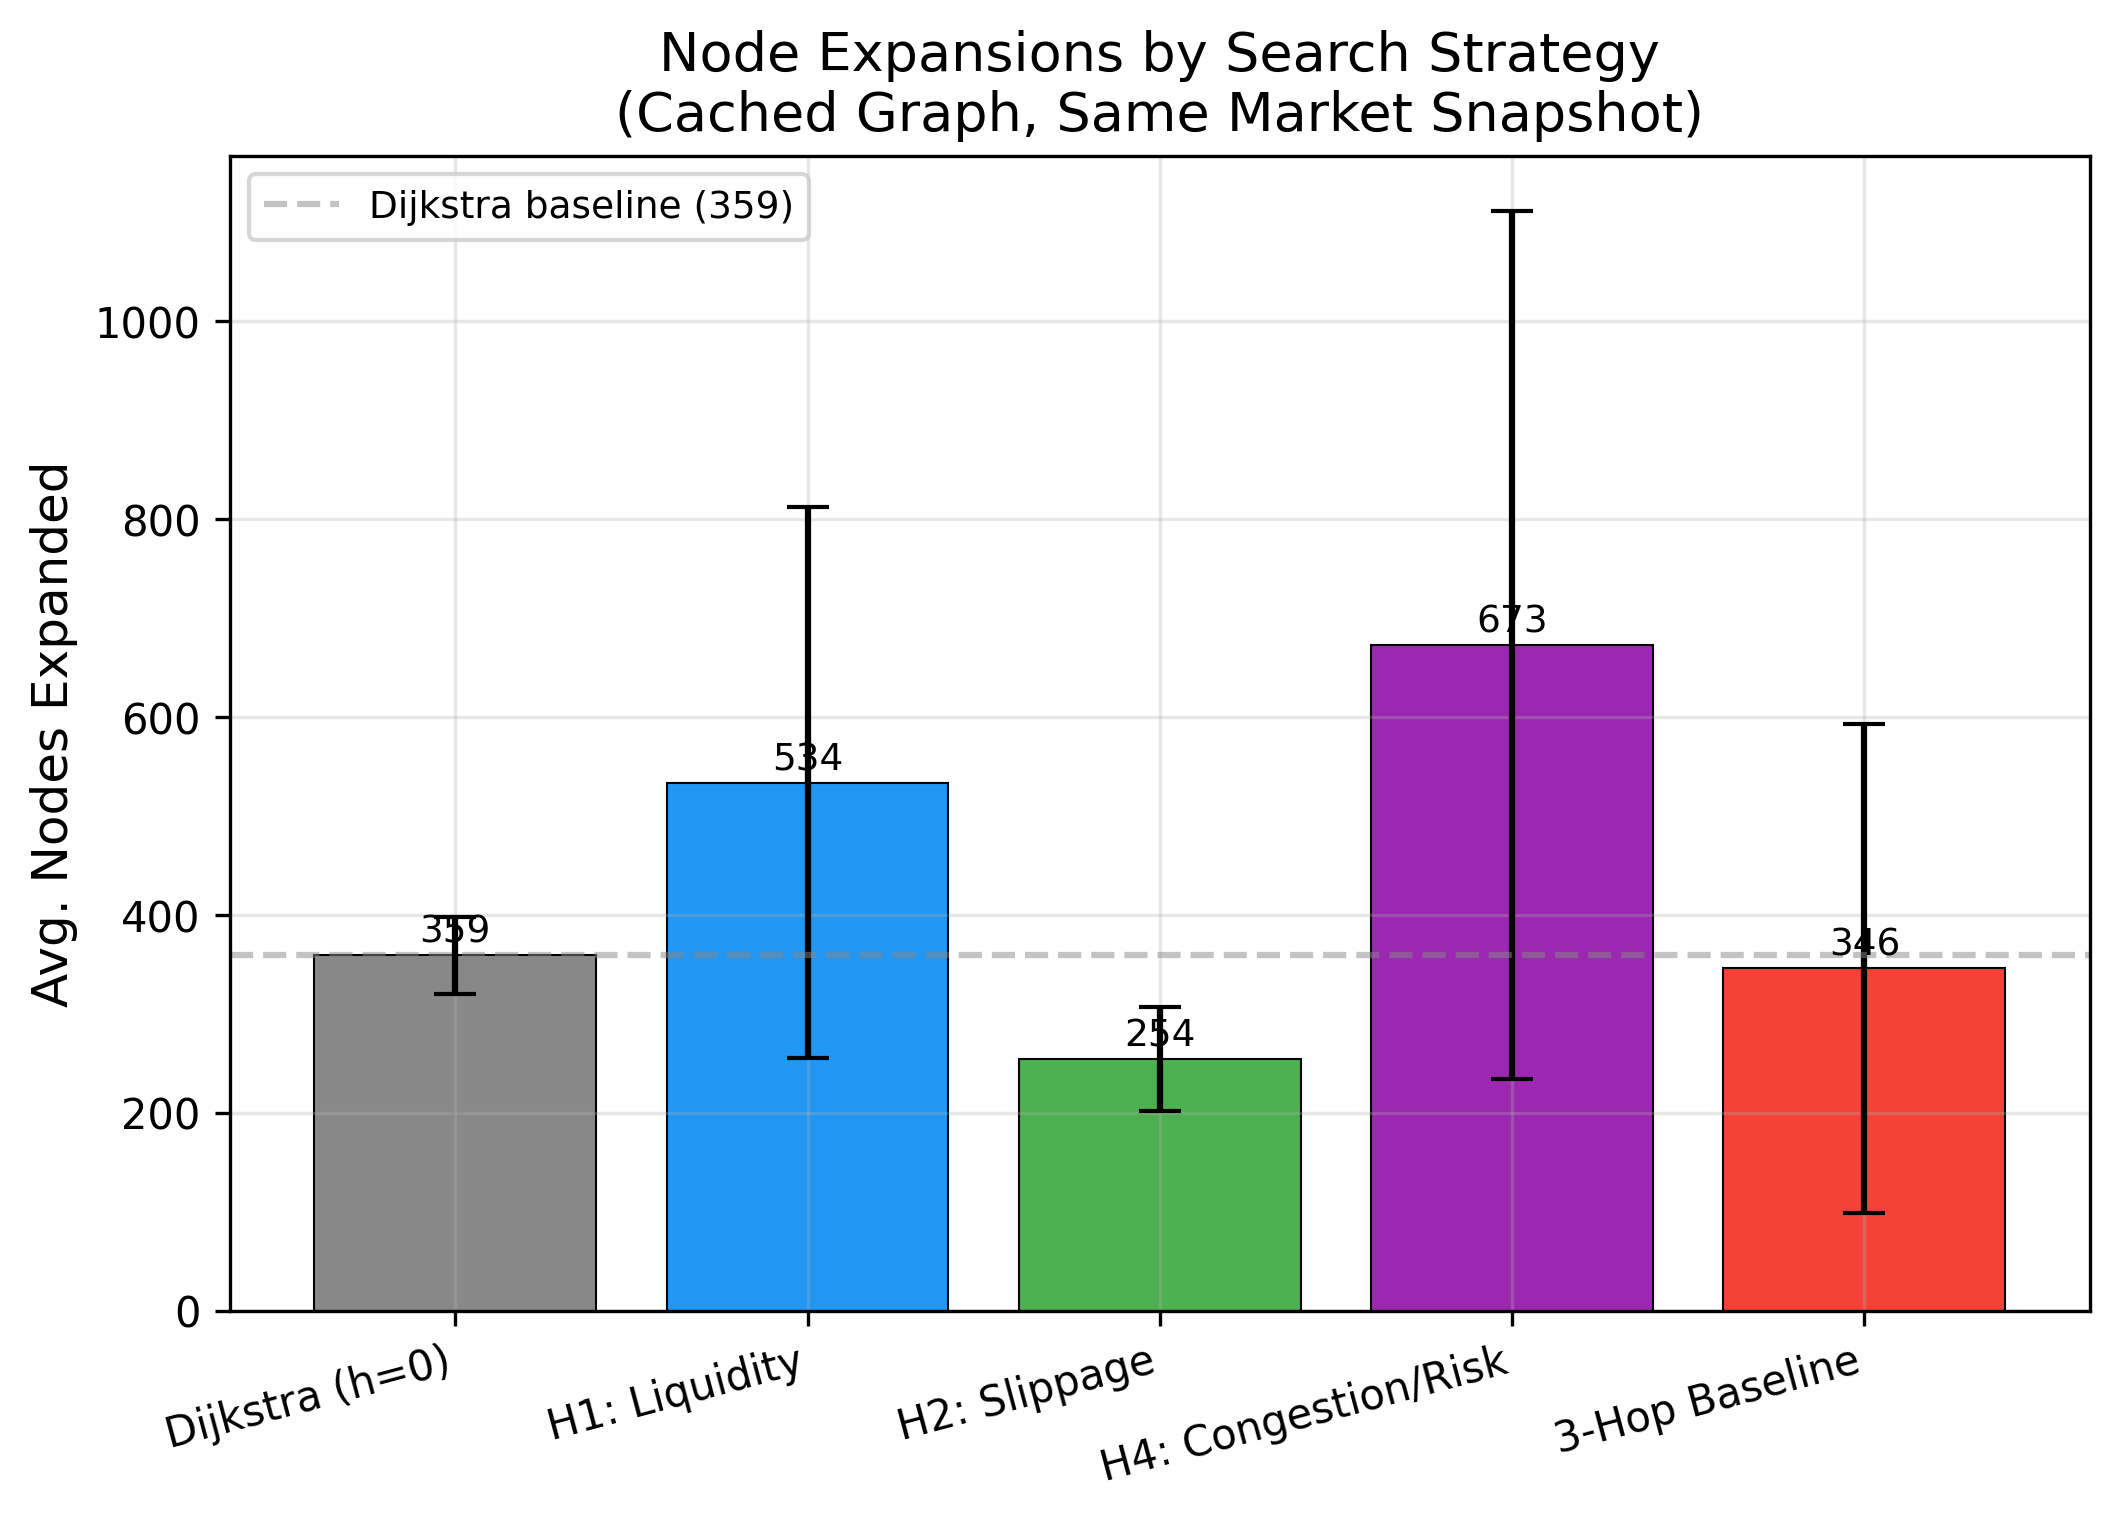
\includegraphics[width=\textwidth]{figures/fig01_node_expansion_bar.png}
    \caption{Mean node expansions by heuristic.}
\end{subfigure}
\hfill
\begin{subfigure}[t]{0.48\textwidth}
    \centering
    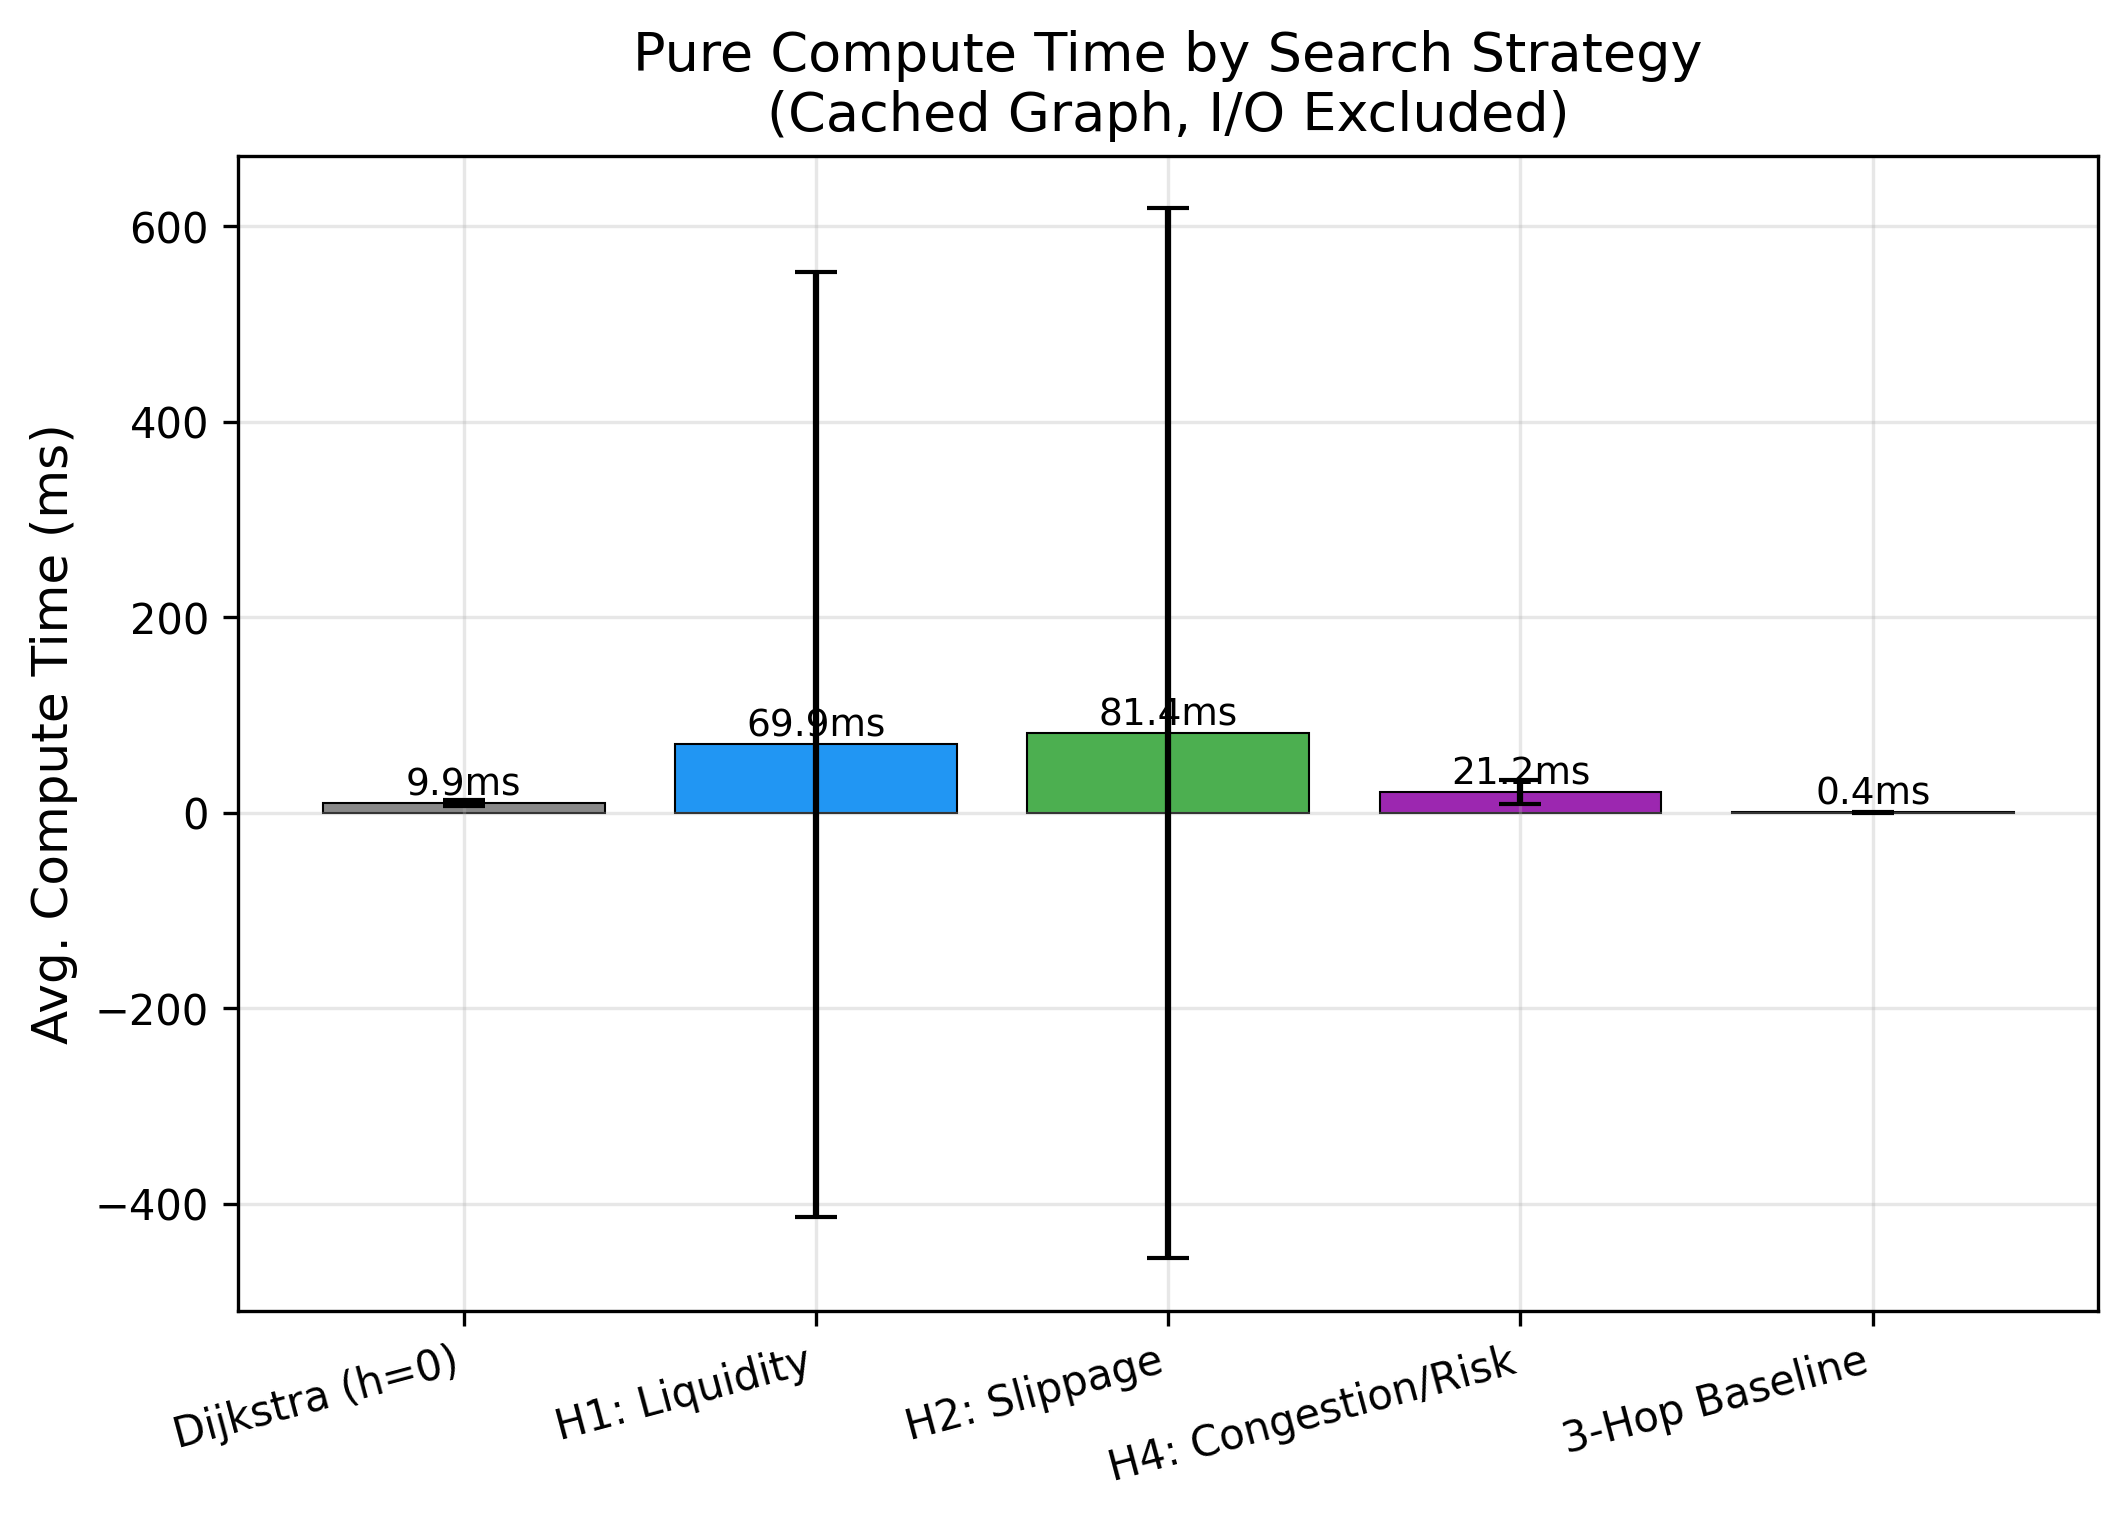
\includegraphics[width=\textwidth]{figures/fig02_compute_time_bar.png}
    \caption{Mean compute time by heuristic.}
\end{subfigure}
\caption{Heuristic comparison on cached graph (30~start nodes, 3~cash levels).}
\label{fig:app_expansion_time}
\end{figure}

\paragraph{Overnight temporal evolution.}
Figure~\ref{fig:app_overnight_ts} shows profit trajectories across 96~snapshots (8~hours, 5-min intervals). Profitable opportunities persist throughout the entire session, with profits clustering around 2--3 structural optima per start node. Periodic dips correspond to temporary market equilibria that resolve within minutes.

\begin{figure}[h]
\centering
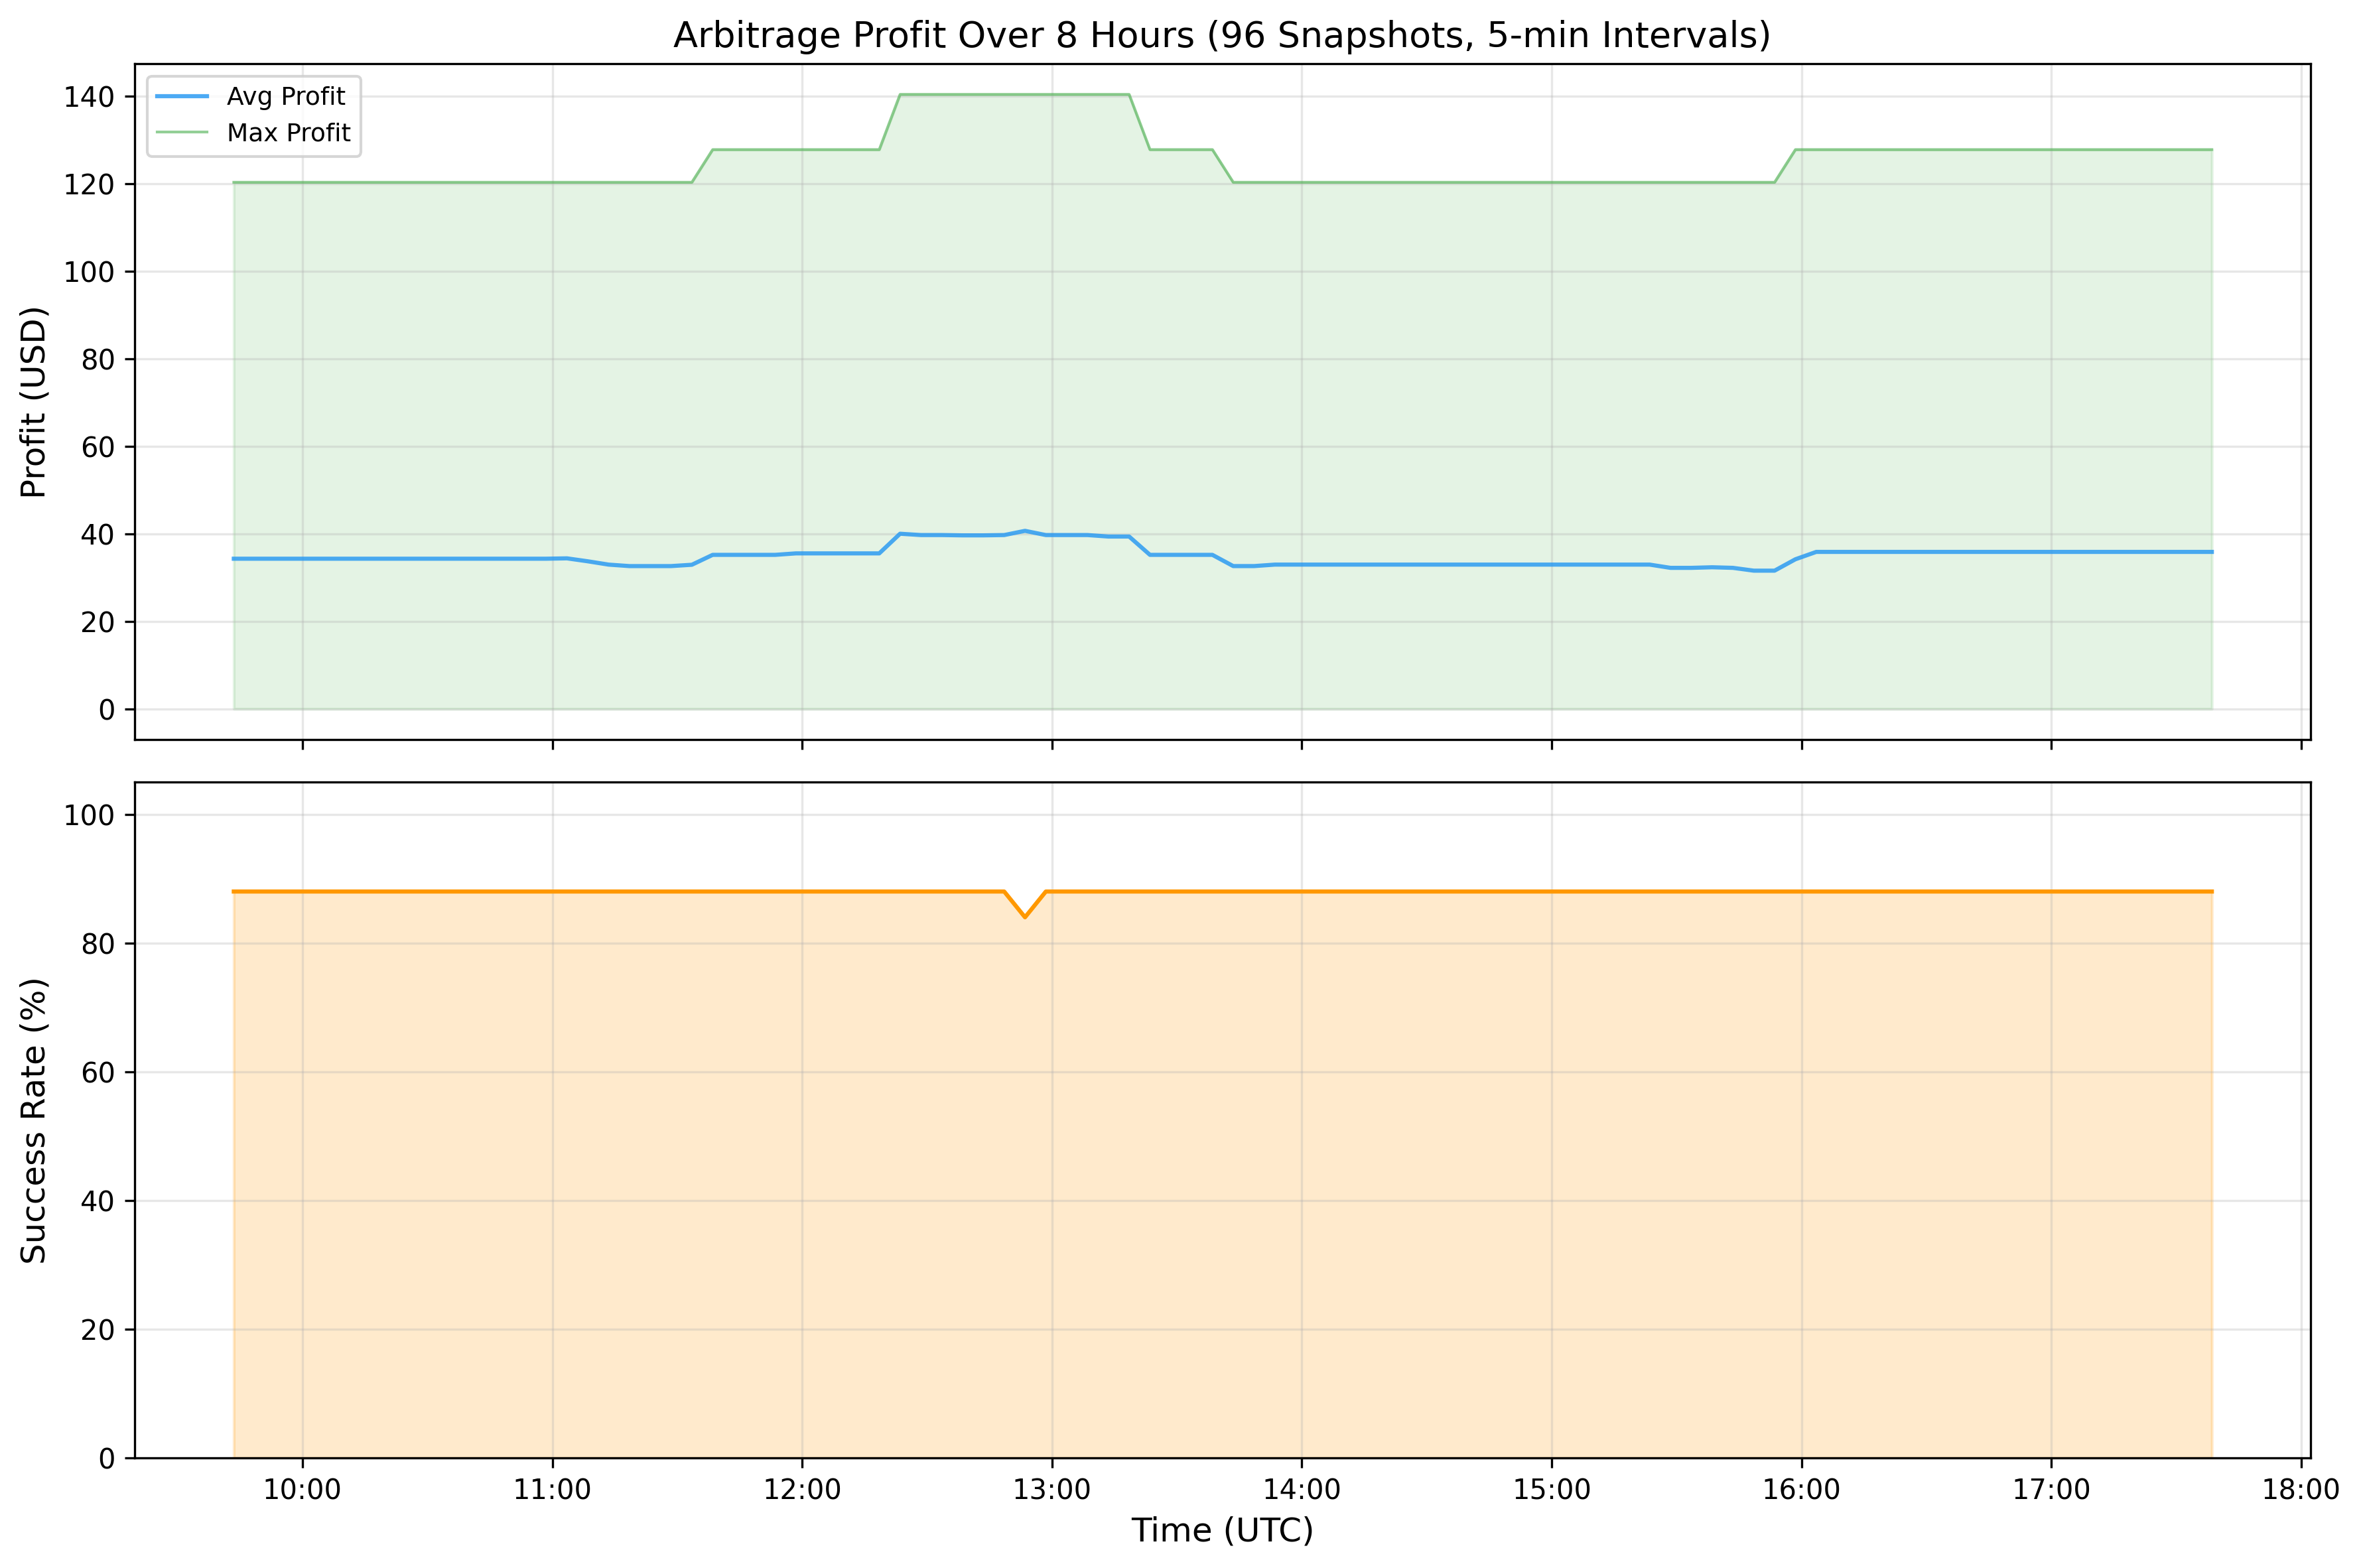
\includegraphics[width=0.85\textwidth]{figures/fig10_overnight_timeseries.png}
\caption{Overnight profit timeseries across all heuristics (8~hours, 5-min intervals, 5~start nodes, 3~cash levels).}
\label{fig:app_overnight_ts}
\end{figure}

\paragraph{Sensitivity: $h_1$ liquidity penalty and max depth.}
Figure~\ref{fig:app_sensitivity_extra} shows that $h_1$ performance is robust across $\lambda_{\text{liq}} \in [0.1, 5.0]$, and that increasing max depth beyond 3 hops yields no additional profit, confirming that profitable stablecoin paths are inherently short.

\begin{figure}[h]
\centering
\begin{subfigure}[t]{0.48\textwidth}
    \centering
    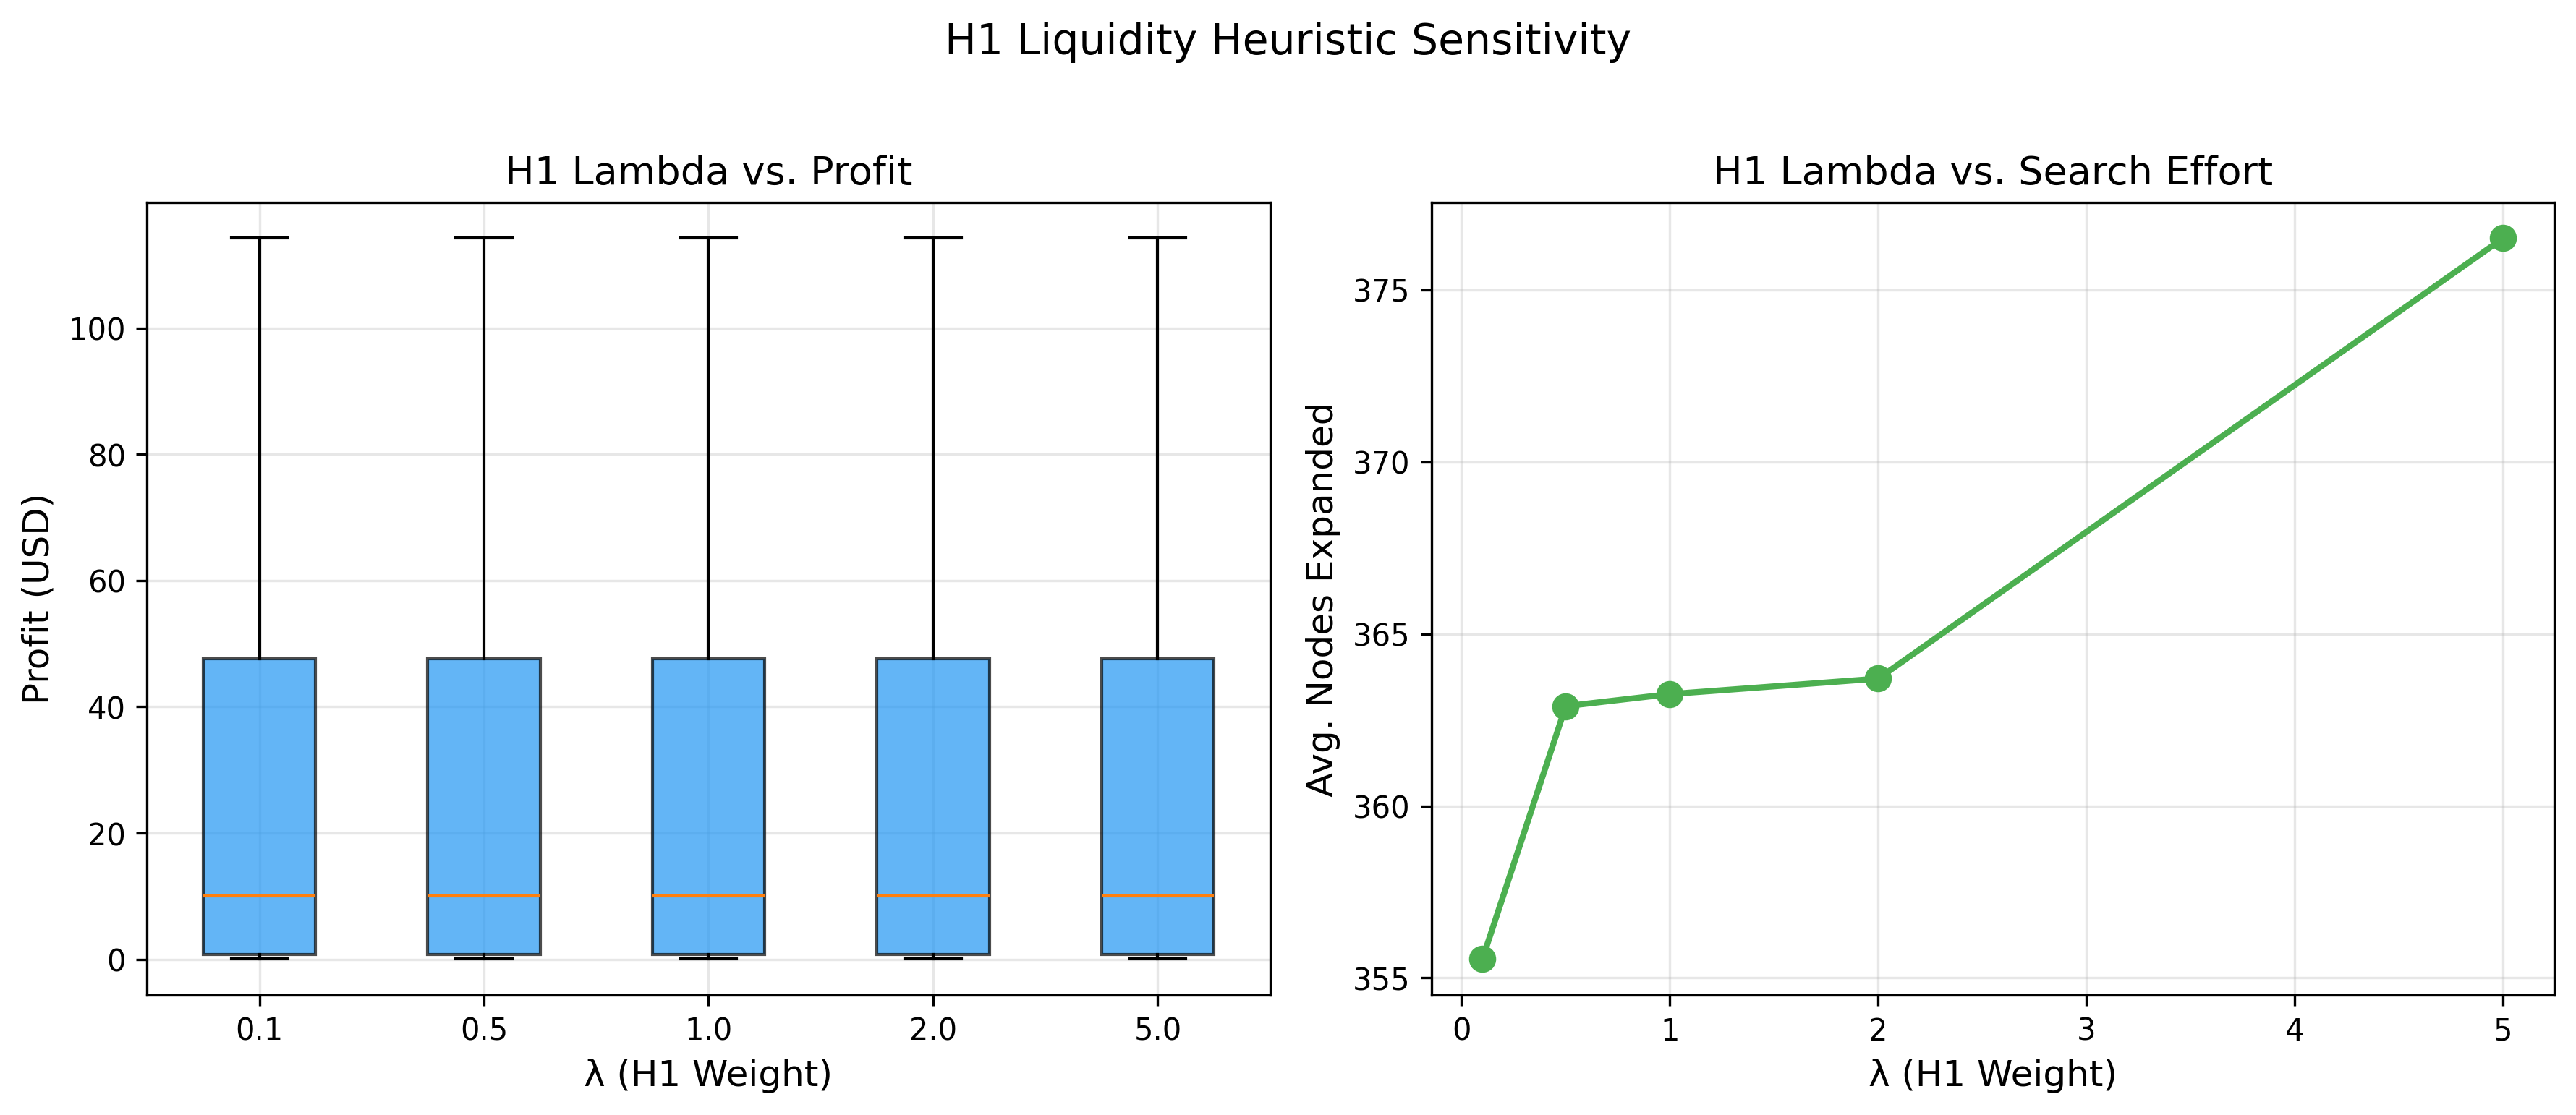
\includegraphics[width=\textwidth]{figures/fig12_sensitivity_h1_lambda.png}
    \caption{$h_1$: profit vs.\ $\lambda_{\text{liq}}$.}
\end{subfigure}
\hfill
\begin{subfigure}[t]{0.48\textwidth}
    \centering
    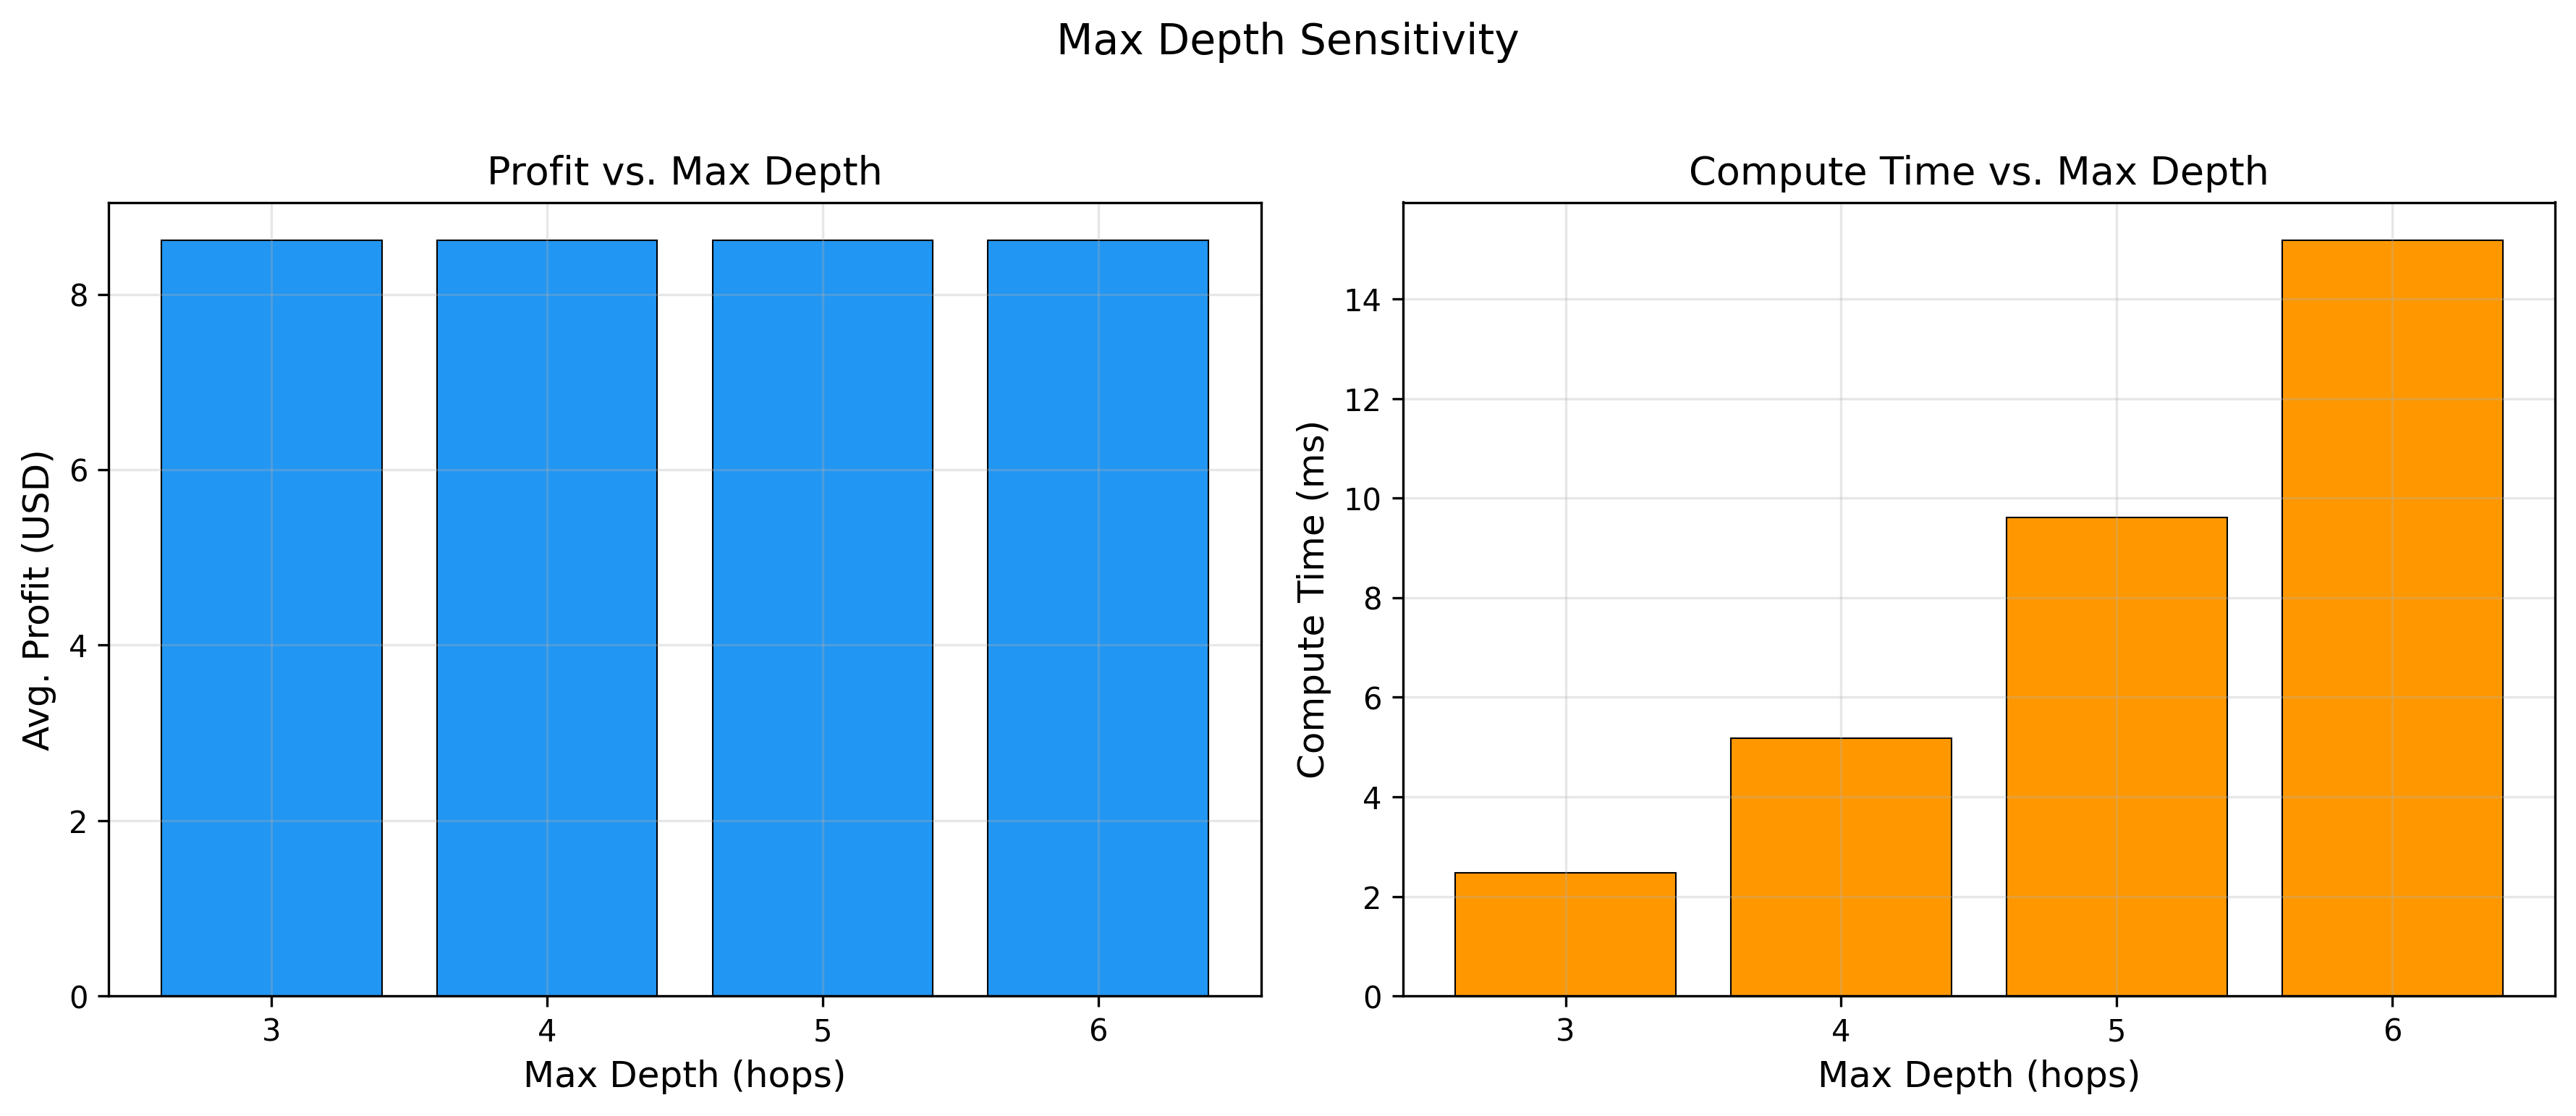
\includegraphics[width=\textwidth]{figures/fig15_sensitivity_max_depth.png}
    \caption{Profit vs.\ max path depth.}
\end{subfigure}
\caption{Additional sensitivity analysis.}
\label{fig:app_sensitivity_extra}
\end{figure}

\paragraph{Radar summary and profit distribution.}
Figure~\ref{fig:app_radar_profit} provides a multi-dimensional summary of heuristic performance across six metrics, alongside the profit distribution across order sizes. $h_4$ dominates on speed and reliability, while $h_2$ leads on expansion efficiency.

\begin{figure}[h]
\centering
\begin{subfigure}[t]{0.48\textwidth}
    \centering
    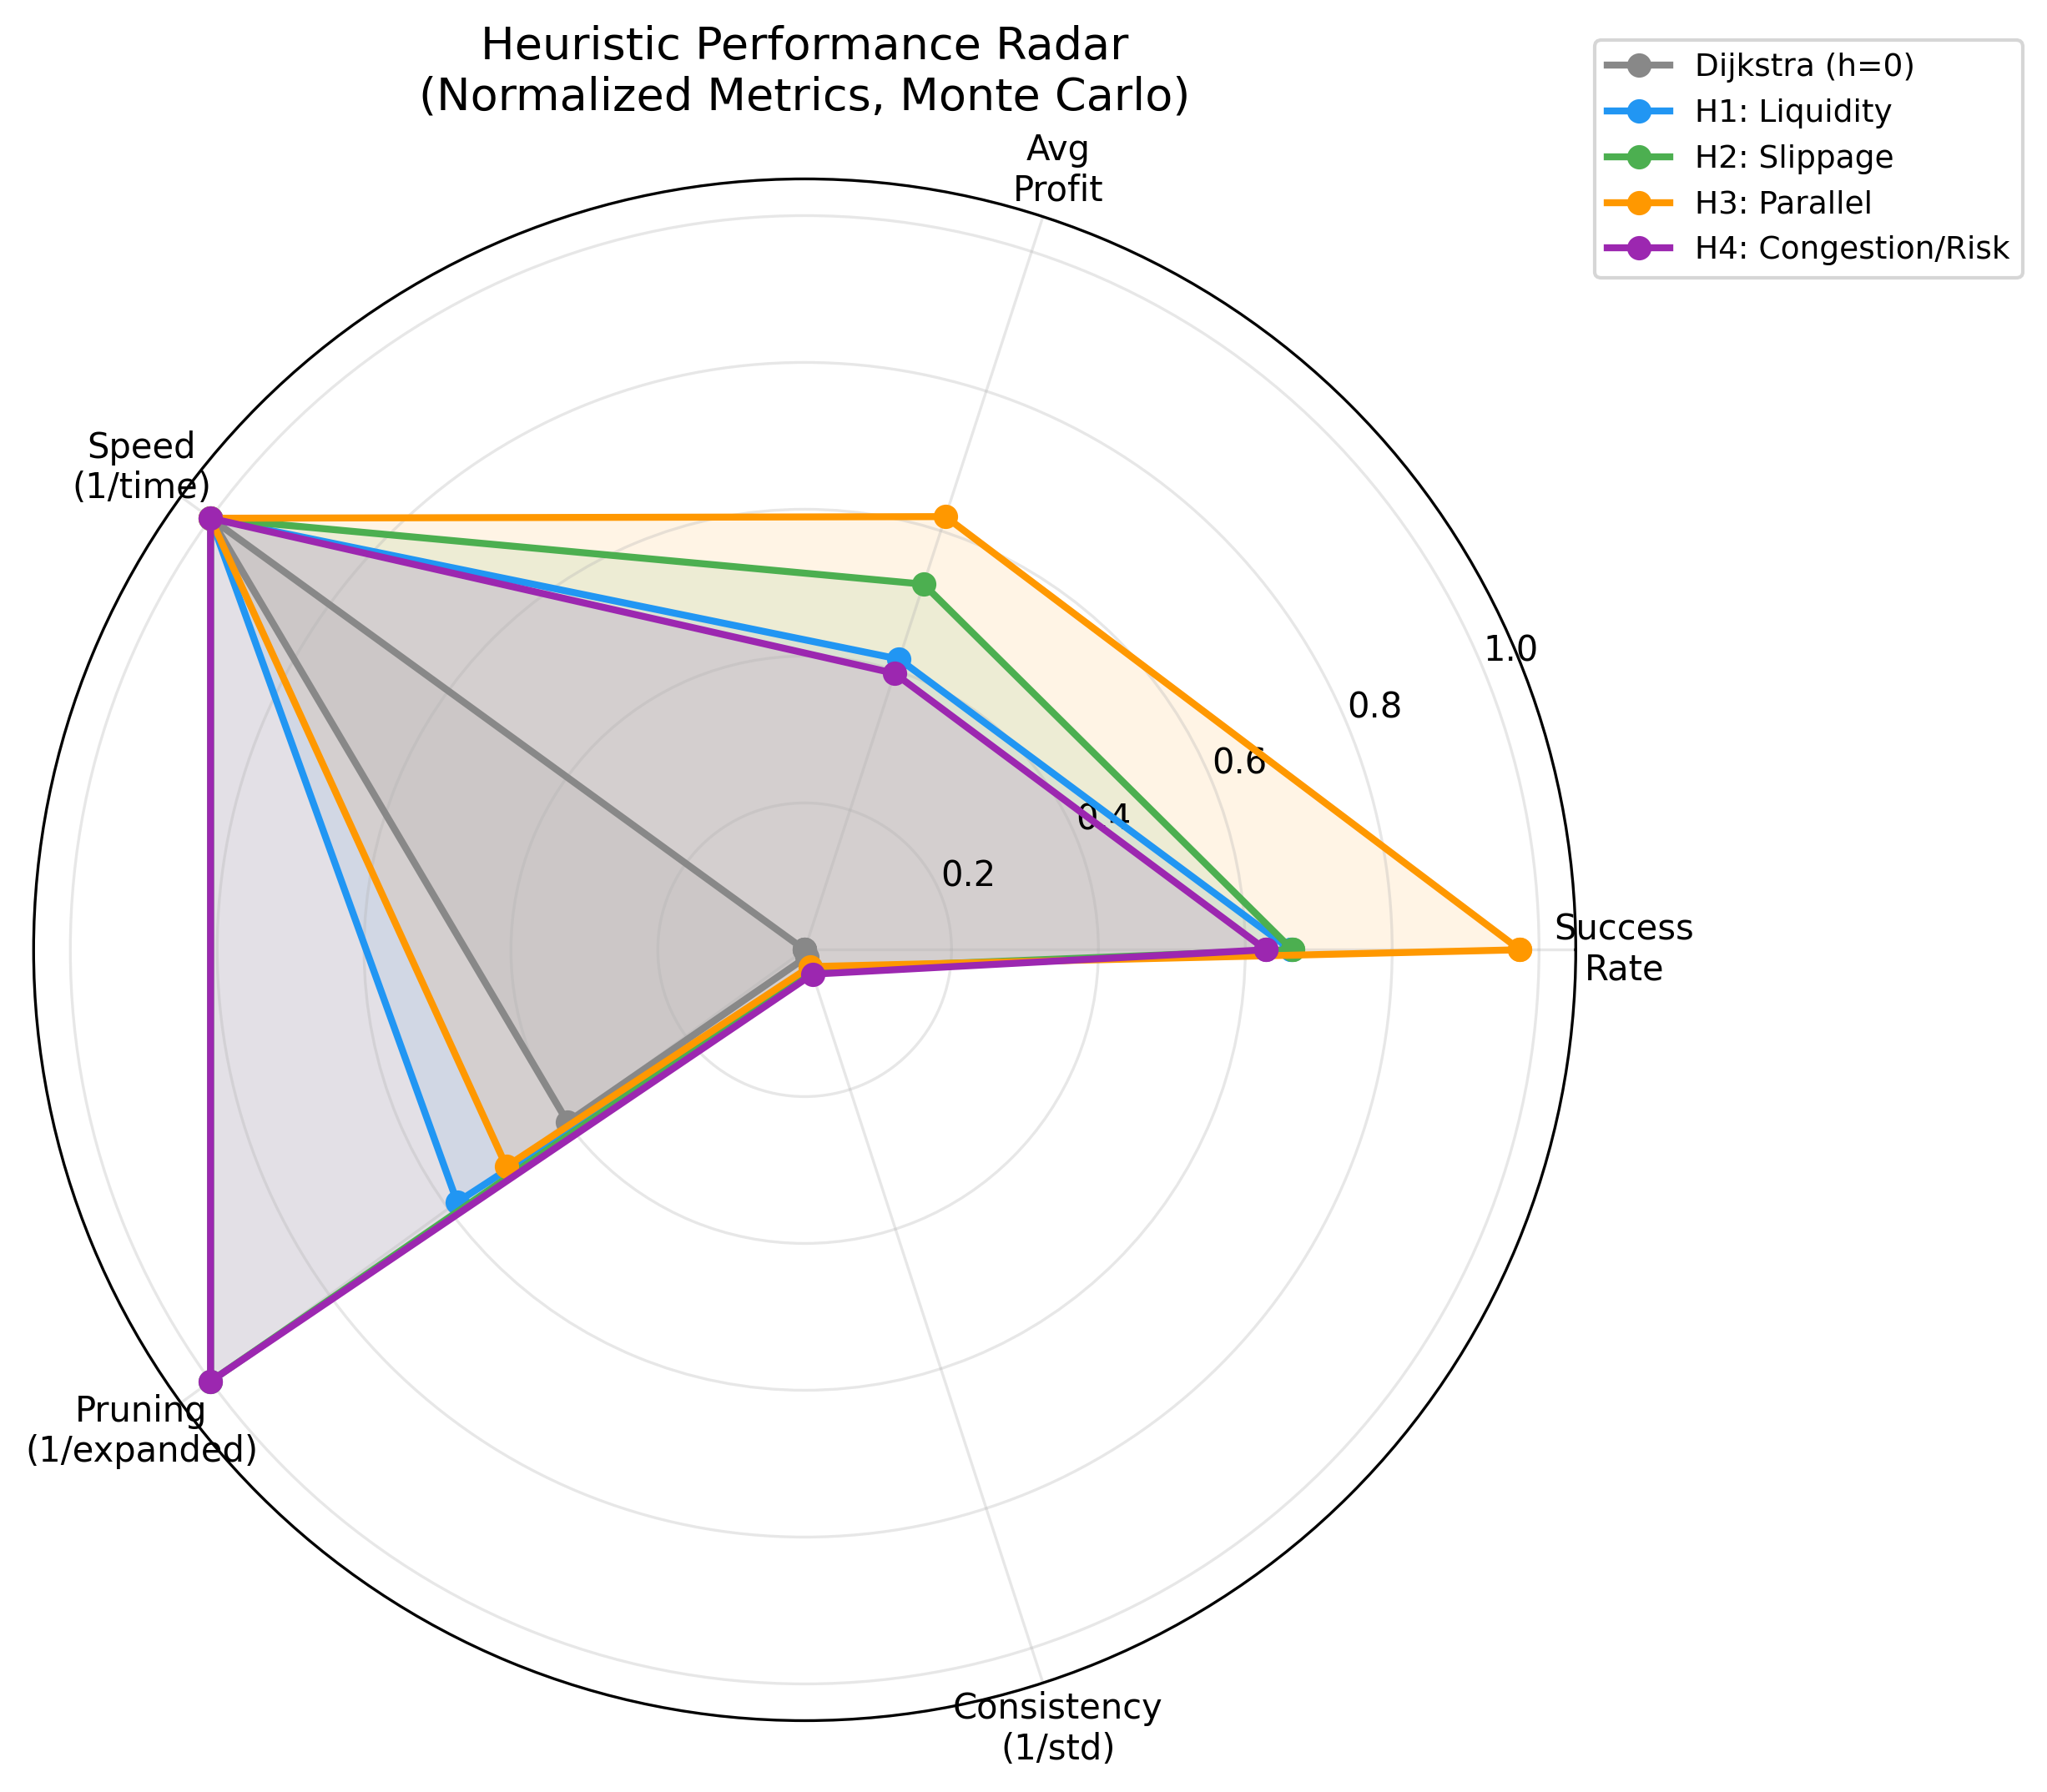
\includegraphics[width=\textwidth]{figures/fig18_radar_summary.png}
    \caption{Radar: multi-metric heuristic comparison.}
\end{subfigure}
\hfill
\begin{subfigure}[t]{0.48\textwidth}
    \centering
    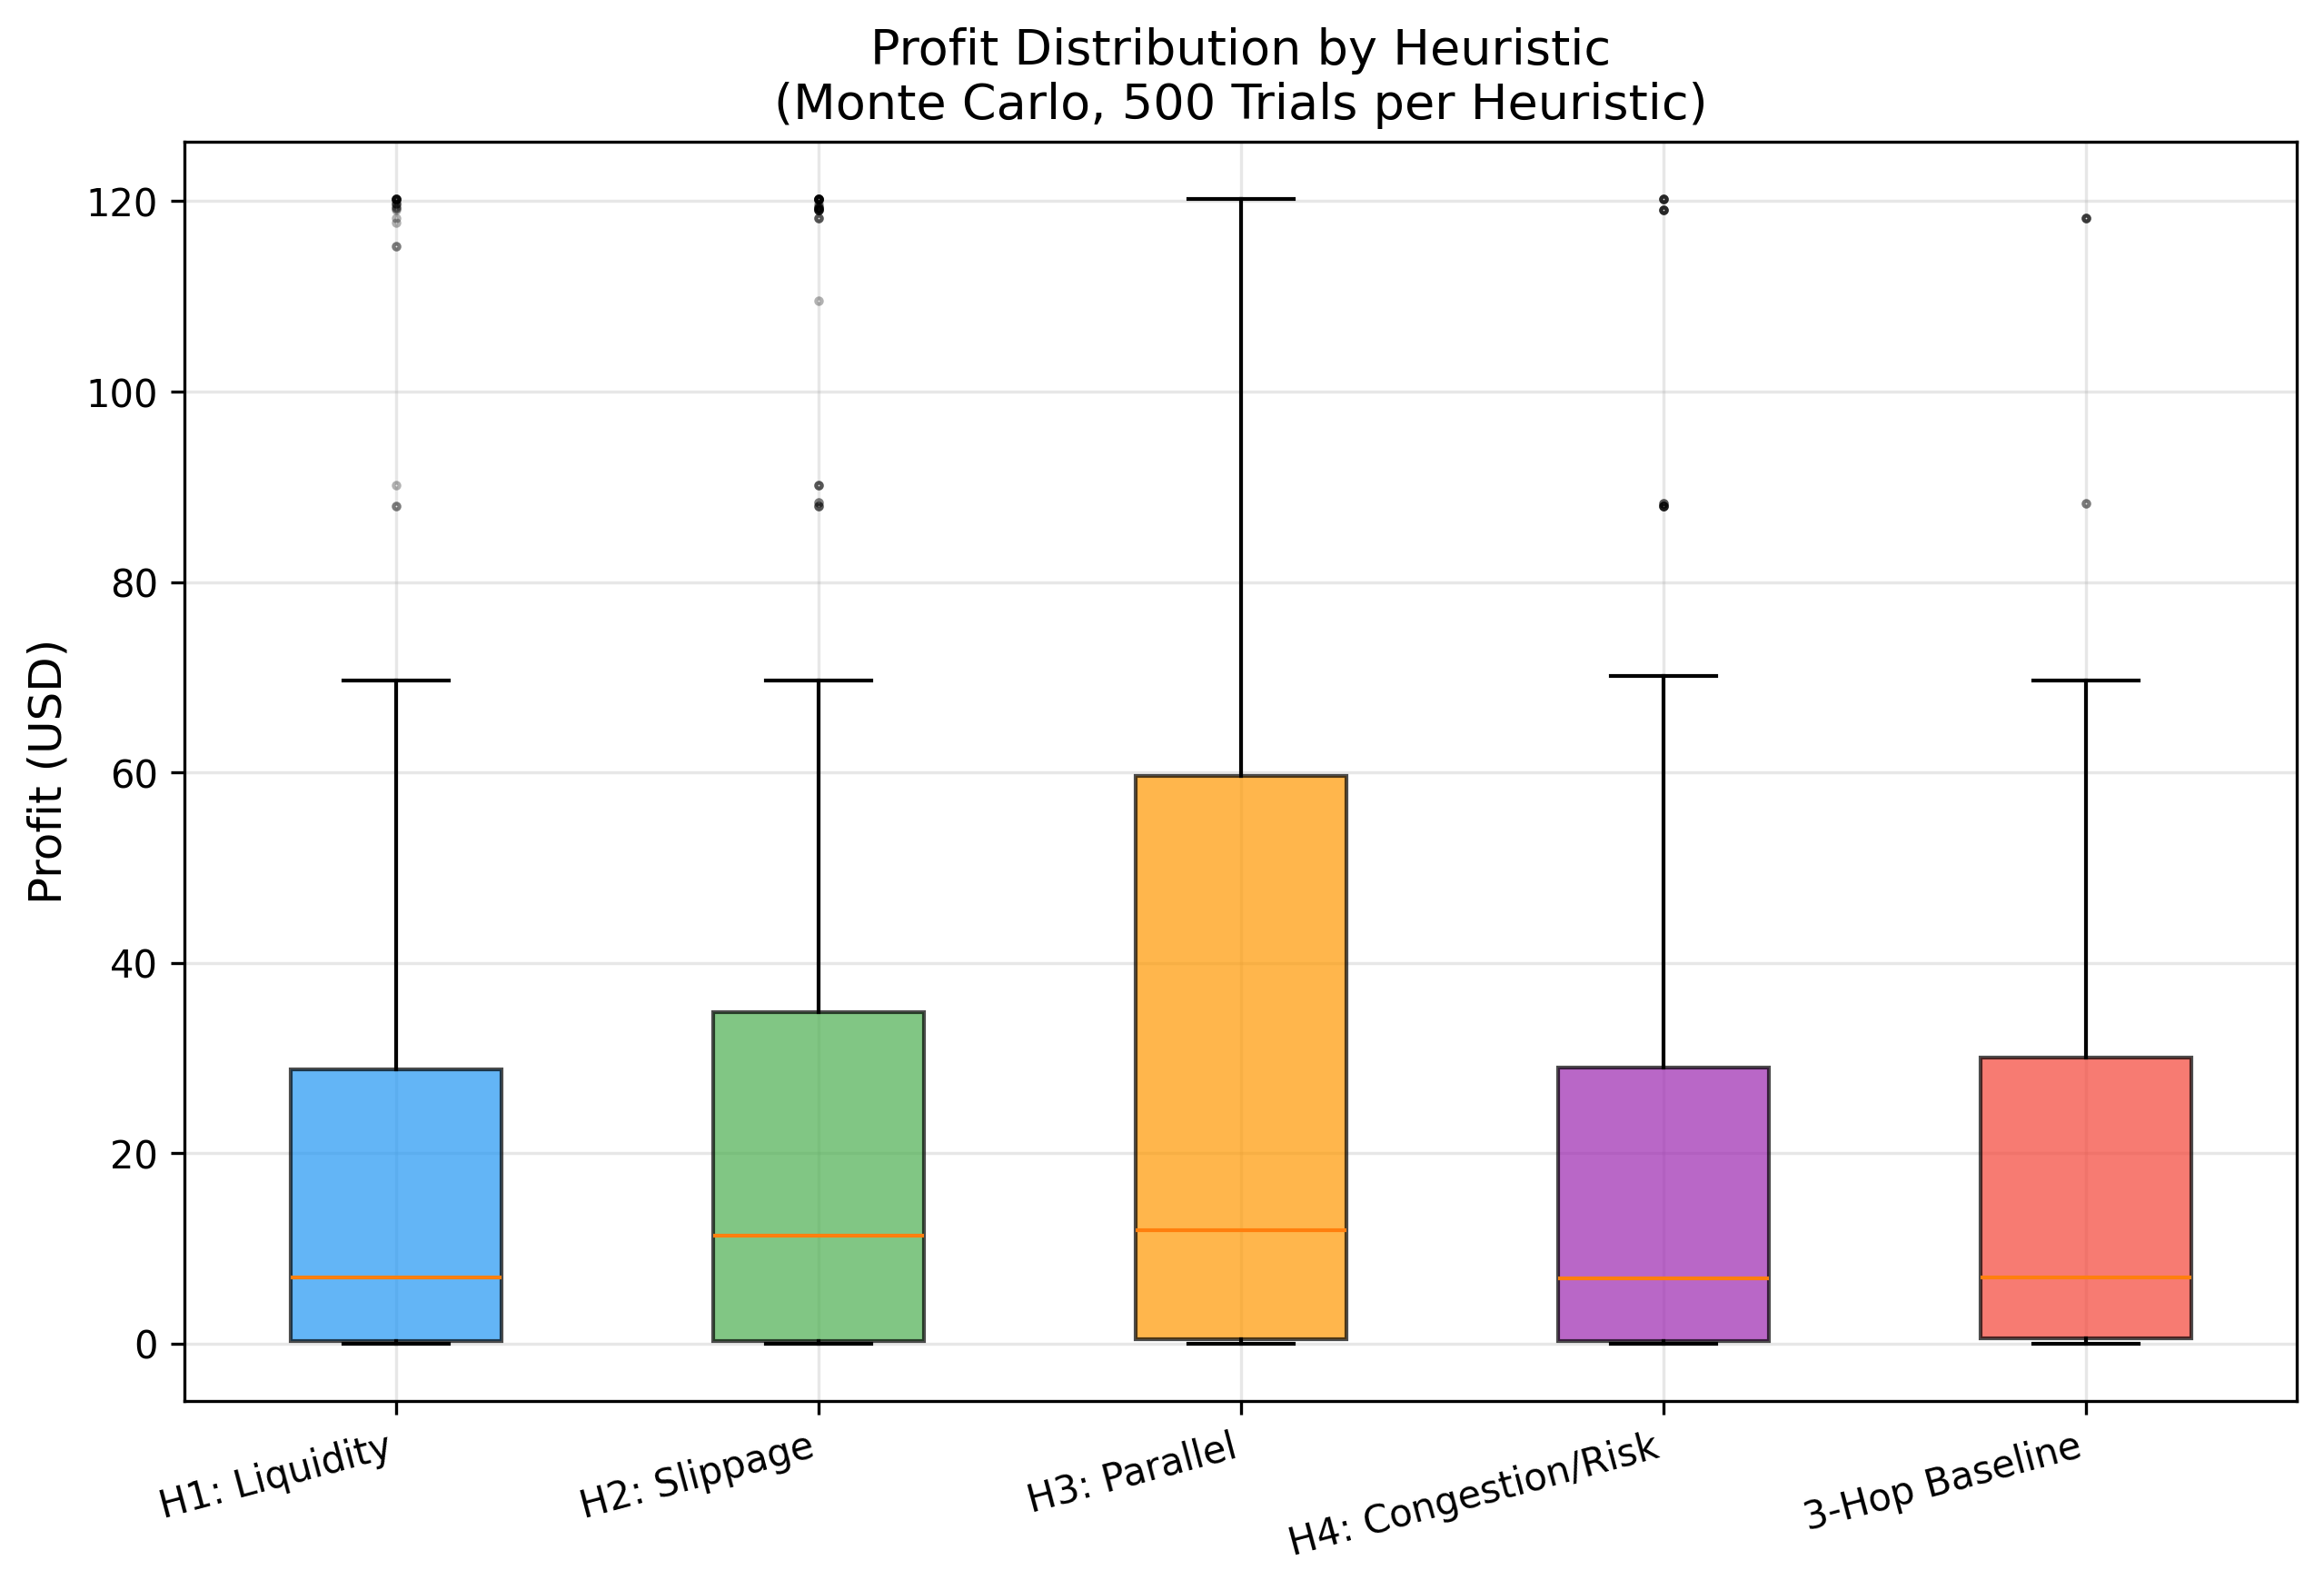
\includegraphics[width=\textwidth]{figures/fig03_profit_boxplot.png}
    \caption{Profit distribution by heuristic.}
\end{subfigure}
\caption{Overall heuristic performance summary.}
\label{fig:app_radar_profit}
\end{figure}

% ============================================================
% A.4 Interactive Visualization System
% ============================================================
\subsection{Interactive Visualization System}
\label{sec:streamlit_ui}

We provide a Streamlit-based web interface for real-time exploration of arbitrage opportunities. The UI integrates live CCXT market data and provides four tabs: (1)~\textbf{Arbitrage Graph} with interactive network visualization, heuristic selection, and search execution with streaming log output; (2)~\textbf{Live Prices} showing real-time stablecoin prices across exchanges; (3)~\textbf{Fees} displaying all fee structures; (4)~\textbf{Documentation}. Upon search completion, results include the complete route, per-node heuristic values, and step-by-step execution details with fees and transfer times. The system uses NetworkX for graph operations and Matplotlib for visualization. Source code is available in the anonymized repository.


\end{document}

